\chapter{The best students, where do they study? A rating case study}
\label{sec:14}

\abstract*{ In 2004, the German magazine \emph{Der Spiegel}, with the help of \emph{McKinsey \& Company} and \emph{AOL}, conducted an extensive online survey, assessing the apparent quality of German University students \citep{SPI-2004}. The eventually published results by the \emph{Spiegel} magazine concerned nearly 50,000 students, enrolled in one of fifteen popular academic subjects, like \emph{German Studies}, \emph{Life Sciences}, \emph{Psychology}, \emph{Law}  or \emph{CS}. Based on this published data, we present and discuss in this chapter, how to \emph{rate} with the help of our \Digraph software resources the apparent global \emph{enrolment quality} of new performance records.}

\abstract{ In 2004, the German magazine \emph{Der Spiegel}, with the help of \emph{McKinsey \& Company} and \emph{AOL}, conducted an extensive online survey, assessing the apparent quality of German University students. The eventually published results by the \emph{Spiegel} magazine concerned nearly 50,000 students, enrolled in one of fifteen popular academic subjects, like \emph{German Studies}, \emph{Life Sciences}, \emph{Psychology}, \emph{Law}  or \emph{CS}. Based on this published data, we present and discuss in this chapter, how to \emph{rate} with the help of our \Digraph software resources the apparent global \emph{enrolment quality} of new performance records.}

\section{The rating problem}
\label{sec:14.1}

In the 2004 \Spiegel survey, more than 80,000 students, by participating, were questioned on their '\emph{Abitur}' and university exams' marks, time of studies and age, grants, awards and publications, IT proficiency, linguistic skills, practical work experience, foreign mobility and civil engagement. Each student received in return a quality score through a specific weighing of the collected data which depended on the subject the student is mainly studying. Publishing only those subject-University combinations, where at least 18 students had correctly filled in the questionnaire, left 41 German Universities where, for at least eight out of the fifteen subjects, an average enrolment quality score could be determined  \citep{SPI-2004,SPI-2004m}.

We suppose in this rating case study that five German universities: \texttt{U1}, \texttt{U2}, \texttt{U3}, \texttt{U4} and \texttt{U5} conducted in 2005 a similar survey among their enrolled students which gave the following enrolment quality scores per academic subject:
\begin{table}[ht]
\caption{Enrolment quality scores per academic subject}
\label{tab:14.1}       % Give a unique label
\begin{center}
  %\begin{small}
    \begin{tabular}{l|c|c|c|c|c}
      \svhline\noalign{\smallskip}
      Subject & U1 & U2 & U3 & U4 & U5 \\
      \noalign{\smallskip}\hline\noalign{\smallskip}
      \texttt{bio}   & NA     & 53.10 & 49.70 & 52.20 & 55.20\\
      \texttt{med}   & NA     & NA    & NA    & 49.50 & 55.50\\
      \              & \      & \     & \     & \     & \    \\
      \texttt{math}  & 56.80  & 54.70 & 56.30 & 58.60 & 61.30\\
      \texttt{phys}  & 58.90  & 59.80 & 53.90 & 59.10 & 60.90\\
      \texttt{chem}  & 52.00  & 50.10 & 54.20 & 53.60 & 56.70\\
      \              & \      & \     & \     & \     & \    \\
      \texttt{germ}  & 51.40  & 53.50 & 51.40 & 53.30 & 61.40\\
      \texttt{pol}   & NA     & 54.00 & NA    & 50.80 & 59.60\\
      \texttt{soc}   & 59.10  & 51.50 & 55.60 & 51.00 & 52.20\\
      \texttt{psy}   & 57.70  & NA    & 54.40 & 62.70 & 59.80\\
      \              & \      & \     & \     & \     & \    \\
      \texttt{law}   & NA     & NA    & 41.90 & NA    & 51.10\\
      \texttt{eco}   & 49.60  & NA    & NA    & NA    & 54.40\\
      \texttt{mgt}   & 54.00  & 53.40 & 50.70 & 49.60 & NA   \\
      \              & \      & \     & \     & \     & \    \\
      \texttt{info}  & 55.40  & 52.60 & 55.80 & 54.60 & NA   \\ 
      \texttt{elec}  & 56.10  & 54.50 & NA    & 57.20 & NA   \\
      \texttt{mec}   & 54.30  & 55.20 & NA    & 54.40 & NA   \\
      \noalign{\smallskip}\hline
    \end{tabular}
  %\end{small}
\end{center}
\end{table}

In Table~\vref{tab:14.1}, the fifteen popular academic subjects are grouped into topical 'Faculties': - \emph{Humanities}; - \emph{Law, Economics \& Management}; - \emph{Life Sciences \& Medicine}; - \emph{Natural Sciences \& Mathematics}; and - \emph{Technology}. None of the five universities has students enrolled in all the fifteen subjects. University U1 has, for instance, no students in Life Sciences \& Medicine, and in Law and Politology. Whereas the University U5 does not offer any Technology subjects.

The average enrolment quality scores of the five universities, shown in Table~\vref{tab:14.1} are stored in a file named \texttt{ratingCaseStudy.py} of \texttt{PerformanceTableau} format\footnote{The file may be found in the \texttt{examples} directory of the \Digraph resources.}. The \texttt{showHTMLPerformanceTableau()}  method produces in Fig.~\vref{fig:14.1} a colourful browser view of these performance records. 
\begin{lstlisting}
>>> from perfTabs import PerformanceTableau
>>> pt = PerformanceTableau('ratingCaseStudy')
>>> pt.showHTMLPerformanceTableau(Transposed=True,\
...                     title='Average enrolment scores')
\end{lstlisting}
\begin{figure}[ht]
\sidecaption[t]
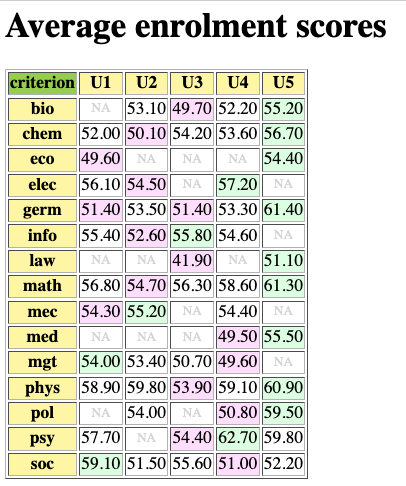
\includegraphics[width=6cm]{Figures/14-1-enrolmentScores.png}
\caption[Student enrolment quality scores per subject]{\emph{Student enrolment quality scores per subject}\\ The light green, resp. light red, figures indicate highest, resp. lowest, score among the five universities.}
\label{fig:14.1}       % Give a unique label
\end{figure}

With the best score in nine out of fifteen subjects, university \texttt{U5} presents the highest global enrolment quality of the five, whereas university \texttt{U3}, with five lowest scores, shows the lowest student enrolment quality of the five.

The university administrations would like to know now how their respective enrolment quality scores are to be appreciated in view the results of the 2004 \Spiegel survey. Are they among the top universities, the midfield or the bottom group?

\section{The 2004 performance quintiles}
\label{sec:14.2}

The estimated lower-closed performance quintiles of the 2004 average enrolment quality per academic subject are stored in a file named \texttt{historicalQuan\-tiles.py}\footnote{The file may be found in the \texttt{examples} directory of the \Digraph resources.} which can be reloaded with the \texttt{PerformanceQuantiles} class.\index{PerformanceQuantiles@\texttt{PerformanceQuantiles} class}.
\begin{lstlisting}[caption={Inspecting stored historical performance quantiles},label=list:14.1]
>>> from performanceQuantiles import PerformanceQuantiles
>>> pq = PerformanceQuantiles('historicalQuintiles')
>>> pq
  *---- PerformanceQuantiles instance description ---*
   Instance class   : PerformanceQuantiles
   Instance name    : historicalQuintiles
   Objectives       : 4
   Criteria         : 15
   Quantiles        : 5
   History sizes    : {'germ': 39, 'pol': 34, 'psy': 34,
                       'soc': 32, 'law': 32, 'eco': 21,
                       'mgt': 34, 'bio': 34, 'med': 28,
                       'phys': 37, 'chem': 35, 'math': 27,
                       'info': 33, 'elec': 14, 'mec': 13}
   Attributes       : ['name', 'objectives', 'NA', 'criteria',
                       'quantilesFrequencies', 'historySizes',
                       'LowerClosed', 'limitingQuantiles',
                       'cdf', 'perfTabType']
\end{lstlisting}

The history sizes, reported in Listing~\vref{list:14.1}, indicate the number of Universities evaluated in the 2004 survey in each one of the popular fifteen subjects. German Studies, for instance, were evaluated for 39 out of 41 Universities, whereas Electrical and Mechanical Engineering were only evaluated for 14, respectively 13 Institutions. None of the fifteen subjects were evaluated in all the 41 Universities \footnote{It would have been interesting to estimate such quantile limits from the individual quality scores of all the nearly 50,000 surveyed students. But this data was not public \citep{SPI-2004}.}.                      

Details of the fifteen academic subjects --the performance criteria-- may be consulted in a browser view (see Fig.~\vref{fig:14.2}).
\begin{lstlisting}
>>> pt.showHTMLCriteria()
\end{lstlisting}
\begin{figure}[ht]
%\sidecaption
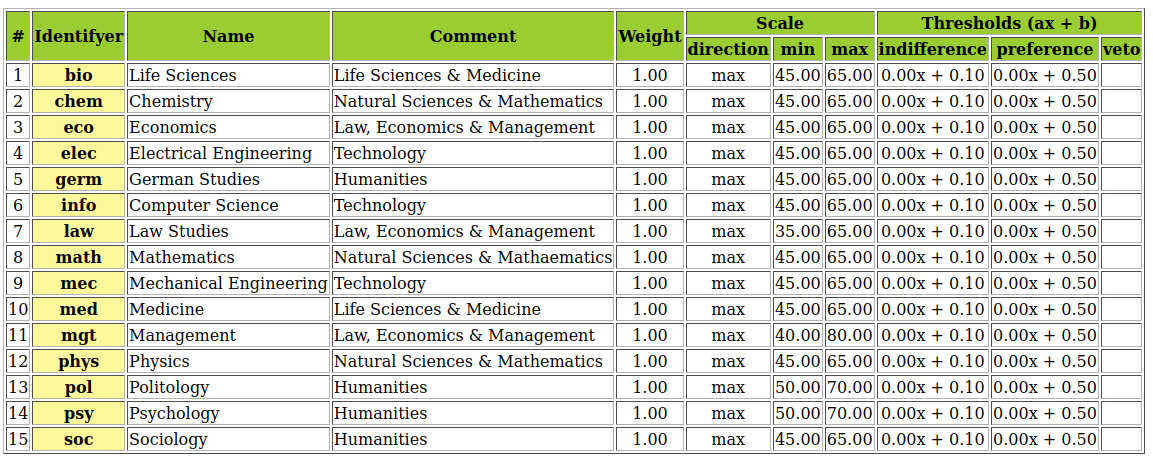
\includegraphics[width=\hsize]{Figures/14-2-spiegelCriteria.png}
\caption[Fifteen popular academic subjects]{The fifteen academic subjects taken into account for assessing the student enrolment quality}
\label{fig:14.2}       % Give a unique label
\end{figure}

All fifteen subjects are considered equally significant (see Column Weight). The average scores in most subjects vary from 45 to 65. In some subjects, however, like Law Studies ($35.0 - 65-0$) and Politology ($50.0 - 70.0$) a different variability is observed. The average enrolment scores per subject are hence incommensurable and global average enrolment scores over all subjects become meaningless. 

To take furthermore into account the potential and very likely imprecision of the quality scores' computation, we assume that, for all subjects, an average enrolment quality score difference of $0.1$ is \emph{insignificant}, whereas a difference of $0.5$ is sufficient to positively attest a \emph{better} enrolment quality. No considerable performance difference are assumed.

The \texttt{showLimitingQuantiles()} method\index{showLimitingQuantiles@\texttt{showLimitingQuantiles()}} prints in Listing~\vref{list:14.2} the estimated quintile limits of the 2004 survey.
\begin{lstlisting}[caption={Estimated quintile limits of the 2004 survey},label=list:14.2,basicstyle=\ttfamily\scriptsize]
>>> pq.showLimitingQuantiles()
  *----  performance quantiles -----*
  criteria | weights |  '0.00'  '0.20'  '0.40'  '0.60'  '0.80'  '1.00'   
  ---------|----------------------------------------------------------
   'bio'   |   1.0   |   45.00   50.40   51.80   53.14   55.04   57.10  
   'chem'  |   1.0   |   45.00   53.30   54.20   55.80   57.40   58.80  
   'eco'   |   1.0   |   49.60   52.14   53.38   54.28   56.94   60.80  
   'elec'  |   1.0   |   50.10   54.08   55.34   56.54   57.64   60.20  
   'germ'  |   1.0   |   45.00   52.14   54.02   55.84   57.48   61.40  
   'info'  |   1.0   |   45.00   54.40   55.44   56.68   58.10   59.80  
   'law'   |   1.0   |   39.10   42.30   45.08   46.30   47.26   51.10  
   'math'  |   1.0   |   51.60   56.54   57.76   59.44   61.00   63.10  
   'mec'   |   1.0   |   51.90   54.02   54.48   55.18   56.54   57.80  
   'med'   |   1.0   |   45.00   49.20   49.84   51.10   52.42   60.10  
   'mgt'   |   1.0   |   47.50   52.16   52.98   54.68   55.96   68.00  
   'phys'  |   1.0   |   53.90   58.78   59.90   60.96   61.96   62.80  
   'pol'   |   1.0   |   50.80   54.62   56.18   57.78   59.78   65.90  
   'psy'   |   1.0   |   52.50   57.58   58.46   59.80   60.94   64.10  
   'soc'   |   1.0   |   45.00   51.70   53.92   55.42   56.26   59.80  
\end{lstlisting}
                     
We see confirmed again the incommensurability between the subjects, we noticed already in the apparent enrolment quality scoring, especially between Law Studies ($39.1 - 51.1$) and Politology ($50.5 - 65.9$). \footnote{The \emph{Spiegel} authors opted therefore for a simple 3-tiling of the Universities per evaluated academic subject, followed by an average \Borda scores based global ranking \citep{SPI-2004}.}


\section{Rating-by-ranking with lower-closed quintile limits}
\label{sec:14.3}


We add, now, the estimated quintile limits to the enrolment quality records of the 5 Universities and rank, by using the \Copeland rule, all these records conjointly together with the help of the \texttt{LearnedQuantilesRatingDigraph} class\index{LearnedQuantilesRatingDigraph@\texttt{LearnedQuantilesRatingDigraph} class} from the \texttt{sortingDigraphs} module\index{sortingDigraphs@\texttt{sortingDigraphs} module}.
\begin{lstlisting}
>>> from sortingDigraphs import\
...                 LearnedQuantilesRatingDigraph
>>> lqr = LearnedQuantilesRatingDigraph(pq,pt,\
...                 rankingRule='Copeland')
>>> lqr
  *-----  Object instance description -----------*
   Instance class      : LearnedQuantilesRatingDigraph
   Instance name       : learnedRatingDigraph
   Criteria            : 15
   Quantiles           : 5
   Lower-closed bins   : True
   New actions         : 5
   Size                : 44
   Determinateness (%) : 77.6
   Ranking rule        : Copeland
   Ordinal correlation : +0.97
\end{lstlisting}

The resulting ranking of the 5 Universities including the lower-closed quintile score limits may be well illustrated  with the \texttt{showHTMLRatingHeatmap()} method.\index{showHTMLRatingHeatmap@\texttt{showHTMLRatingHeatmap()}}
\begin{lstlisting}
>>> lqr.showHTMLRatingHeatmap(colorLevels=5,\
...              Correlations=True,\
...              ndigits=1,rankingRule='Copeland')
\end{lstlisting}
\begin{figure}[ht]
% %\sidecaption
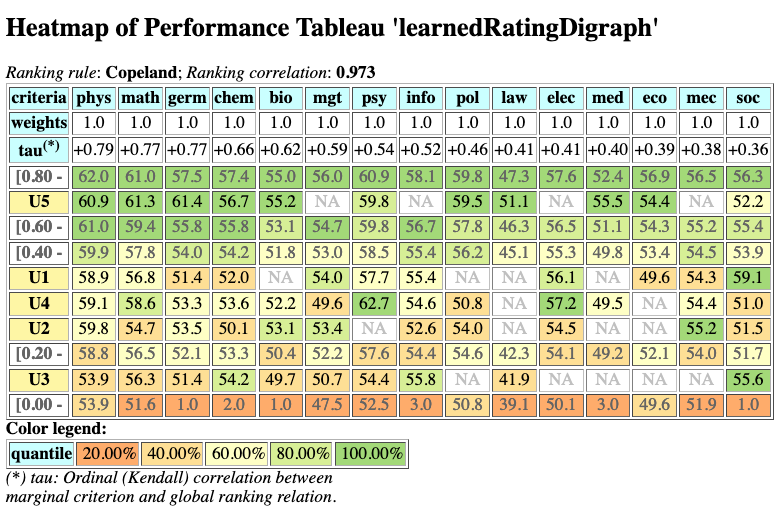
\includegraphics[width=\hsize]{Figures/14-3-quintilingResult.png}
\caption{Heatmap view of the quintiles rating-by-ranking result}
\label{fig:14.3}       % Give a unique label
\end{figure}

The ordinal correlation ($+0.97$) of the \Copeland ranking with the underlying bipolar-valued outranking digraph is very high (see Fig.~\vref{fig:14.3} Row 1). Most correlated subjects with this \emph{rating-by-ranking} result appear to be Physics ($+0.79$), Mathematics ($+0.77$) and German Studies ($+0.77$). Sociology ($+0.36$) is the less correlated subject (see Row 4).

From the actual ranking position of the lower 5-tiling limits, we may now immediately deduce the quintile enrolment quality equivalence classes. No university reaches the highest quintile ($[0.80 - [$), whereas \texttt{U3} is rated into the lowest quintile ($[0.00- 0.20[$). The other three universities U1, U2 and U4 are rated in the second quintile ($[0.20- 0.40[$). The rating result may be easily printed out with the \texttt{showQuantilesRating()} method\index{showQuantilesRating@\texttt{showQuantilesRating()}}.
\begin{lstlisting}[caption={Showing the quintiling of the enrolment quality of the 5 Universities},label=list:14.3]
>>> lqr.showQuantilesRating()
  *---- Quantiles rating result ----*
   [0.60 - 0.80[ ['U5']
   [0.20 - 0.40[ ['U1', 'U4', 'U2']
   [0.00 - 0.20[ ['U3']
\end{lstlisting}

A corresponding \emph{graphviz} drawing with the special \texttt{exportRatingByRan\-kingGraphViz()} method\index{exportRatingByRankingGraphViz@\texttt{exportRatingByRankingGraphViz()}} may well illustrate in Fig.~\vref{fig:14.4} these enrolment quality equivalence classes.
\begin{lstlisting}
>>> lqr.exportRatingByRankingGraphViz('ratingResult')
  *---- exporting a dot file for GraphViz tools ---------*
   Exporting to ratingResult.dot
   dot -Grankdir=TB -Tpdf dot -o ratingResult.png
\end{lstlisting}
\begin{figure}[ht]
\sidecaption[t]
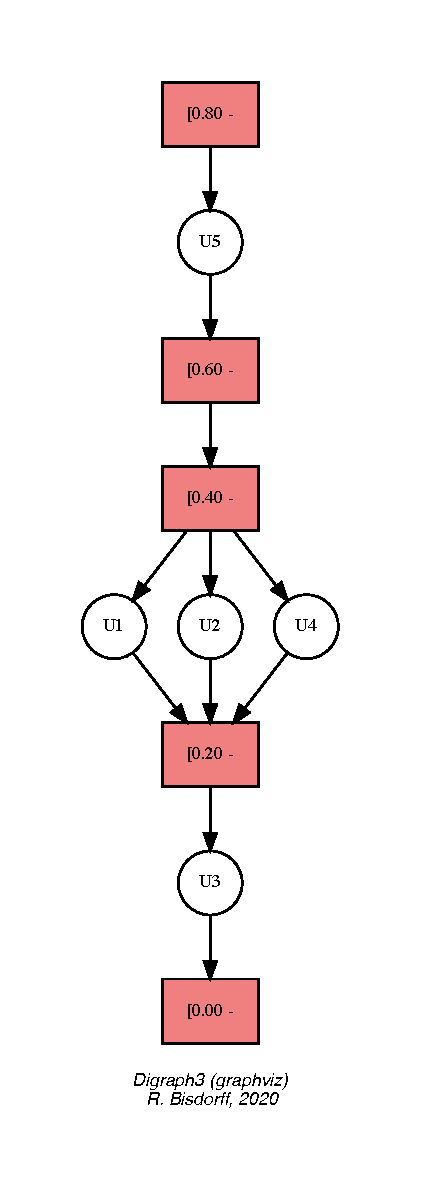
\includegraphics[width=4cm]{Figures/14-4-ratingResult.pdf}
\caption{Drawing of the quintiles rating-by-ranking result}
\label{fig:14.4}       % Give a unique label
\end{figure}
% \clearpage 

We have noticed in Chap.~\ref{sec:8}, that there is not a unique optimal rule for ranking from a given outranking digraph like digraph \texttt{lqr} here. The \Copeland rule, for instance, has the advantage of being \Condorcet consistent, i.e. when the outranking digraph models a linear ranking, this ranking will necessarily be the result of the \Copeland rule. When this is not the case, and especially when the outranking digraph shows chordless circuits, all potential ranking rules may give very divergent ranking results, and sometimes substantially divergent rating-by-ranking results. The \texttt{computeChordlessCircuits()} and \texttt{showChordlessCircuits()} methods allow to check this issue \footnote{The \texttt{computeChordlessCircuits()} and \texttt{showChordlessCircuits()} methods are separate because there are various methods available for enumerating the chordless circuits in a digraph \citep{BIS-2010}.}.
\begin{lstlisting}
>>> lqr.computeChordlessCircuits()
>>> lqr.showChordlessCircuits()
*---- Chordless circuits ----*
1 circuits.
1:  ['U1', 'U2', 'U4'] , credibility : 0.200
\end{lstlisting}

Indeed, there appears an outranking circuit among the three universities \texttt{U1}, \texttt{U2} and \texttt{U4} rated into the 2nd quintile. It is, hence, interesting, to verify if the epistemic fusion of the rating-by-ranking results, one may obtain when applying three different ranking rules, like the \Kemeny, \Copeland and \NetFlows rules, does actually confirm our rating-by-ranking result shown in Fig.~\vref{fig:14.4}. For this purpose we make use in Listing~\vref{list:14.4} of the \texttt{RankingsFusionDigraph} class \index{RankingsFusionDigraph@\texttt{RankingsFusionDigraph} class}.
\begin{lstlisting}[caption={Computing the epistemic fusion of three rating-by-rankig results},label=list:14.4]
>>> # lqr.actionsRanking is Copeland ranked
>>> from linearOrders import KemenyOrder,\
...                          NetFlowsOrder
>>> ke = KemenyOrder(lqr,orderLimit=10)
>>> nf = NetFlowsOrder(lqr)
>>> from transitiveDigraphs import\
...                RankingsFusionDigraph
>>> rankings = [lqr.actionsRanking,\
...             nf.netFlowsRanking,\
...             ke.kemenyRanking]
>>> rankings
 [['m5','u5','m4','m3','u1','u2','u4','m2','u3','m1'], §\label{line:14.4.12}§
  ['m5','u5','m4','m3','u1','u4','u2','u3','m2','m1'],
  ['m5','u5','m4','m3','u1','u4','u2','m2','u3','m1']] §\label{line:14.4.14}§
>>> rf = RankingsFusionDigraph(lqr,rankings)
>>> rf.exportGraphViz(fileName='fusionResult',\
...           WithRatingDecoration=True)
exporting a dot file for GraphViz tools
Exporting to fusionResult.dot
dot -Grankdir=TB -Tpng fusionResult.dot\
                 -o fusionResult.png
\end{lstlisting}
\begin{figure}[ht]
\sidecaption[t]
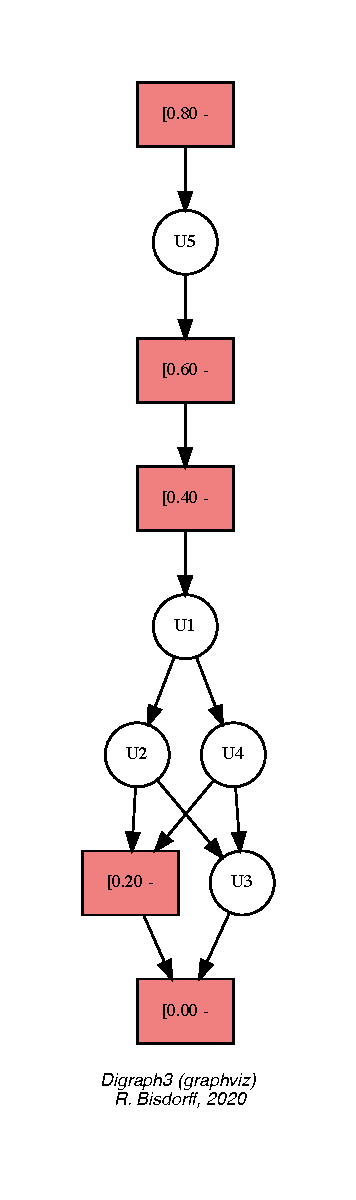
\includegraphics[width=4cm]{Figures/14-5-fusionResult.pdf}
\caption[Disjunctive fusion of the \Kemeny, \Copeland and \NetFlows rankings]{\emph{Disjunctive fusion of the \Kemeny, \Copeland and \NetFlows rankings}\\ They diverge in their rating-by-ranking of Universities \texttt{U2}, \texttt{U3} and \texttt{U4}.}
\label{fig:14.5}       % Give a unique label
\end{figure}

The fusion of the three rating-by-ranking results is shown in Fig.~\vref{fig:14.5} where we see that they diverge solely in their rating-by-ranking of Universities \texttt{U2}, \texttt{U3} and \texttt{U4}. In Listing~\vref{list:14.4} Lines~\ref{line:14.4.12}--\ref{line:14.4.14}, one may more precisely notice that the \Kemeny and \Copeland rules rate \texttt{U3} in the first quintile ($[0.00- 0.20[$), whereas the \NetFlows rule puts \texttt{U3} together with \texttt{U1}, \texttt{U2} and \texttt{U4} into the second quintile ($[0.20- 0.40[$). And, the \Kemeny rule inverts the position of \texttt{U2} and \texttt{U4}.

In Listing~\vref{list:14.5}, the \texttt{showRankingConsensusQuality()} method\index{showRankingConsensusQuality@\texttt{showRankingConsensusQua\-lity()}} reveals finally how fairly \Kemeny and \Copeland rules actually balance the fifteen academic subjects. 
\begin{lstlisting}[caption={Checking the consensus quality of the \Kemeny ranking},label=list:14.5,basicstyle=\ttfamily\scriptsize]
>>> lqr.showRankingConsensusQuality(ke.kemenyRanking)
Consensus quality of ranking:
['m5', 'u5', 'm4', 'm3', 'u1', 'u2', 'u4', 'm2', 'u3', 'm1']
criterion (weight): correlation
-------------------------------
phys (0.067): +0.833
germ (0.067): +0.789
math (0.067): +0.722
bio (0.067): +0.667
mgt (0.067): +0.633
chem (0.067): +0.611
psy (0.067): +0.544
pol (0.067): +0.500
info (0.067): +0.478
mec (0.067): +0.422
law (0.067): +0.411
soc (0.067): +0.400
med (0.067): +0.400
eco (0.067): +0.389
elec (0.067): +0.367
Summary:
Weighted mean marginal correlation (a): +0.544
Standard deviation (b)                : +0.150
Ranking fairness (a)-(b)              : +0.394
\end{lstlisting}

\begin{lstlisting}[caption={Checking the consensus quality of the \Copeland ranking},label=list:14.6,basicstyle=\ttfamily\scriptsize]
>>> lqr.showRankingConsensusQuality(lqr.actionsRanking)
Consensus quality of ranking:
['m5', 'u5', 'm4', 'm3', 'u1', 'u4', 'u2', 'm2', 'u3', 'm1']
criterion (weight): correlation
-------------------------------
phys (0.067): +0.789
math (0.067): +0.767
germ (0.067): +0.767
chem (0.067): +0.656
bio (0.067): +0.622
mgt (0.067): +0.589
psy (0.067): +0.544
info (0.067): +0.522
pol (0.067): +0.456
law (0.067): +0.411
elec (0.067): +0.411
med (0.067): +0.400
eco (0.067): +0.389
mec (0.067): +0.378
soc (0.067): +0.356
Summary:
Weighted mean marginal correlation (a): +0.537
Standard deviation (b)                : +0.148
Ranking fairness (a)-(b)              : +0.389
\end{lstlisting}

The consensus quality of the two rating-by-ranking results do not sensibly differ one of the other. They both show a similar high mean marginal correlation $(+0.544, +0.537)$, similar standard deviations $(+0.150, +0.148)$ and, hence a similar ranking fairness $(+0.394, +0.389)$. 

To furthermore check the quality of our \Copeland rating-by-ranking result, we shall below compute a direct rating-by-sorting into the historic 2004 quintiles of the enrolment quality scores, without making use of any outranking digraph based ranking rule.

\section{Rating by quintiles sorting}
\label{sec:14.4}

In the case study here, the five Universities \texttt{U1}, \texttt{U2}, \texttt{U3}, \texttt{U4} and \texttt{U5} represent the decision actions: \emph{where to study}. We say now that University $x$ is sorted into the lower-closed quintile $k$ when the performance record of $x$ positively outranks the lower limit record $\mathbf{q}(p_{k-1}$ of quintile $q$ and $x$ does not positively outrank the upper limit record $\mathbf{q}(p_{k}$ of quintile $q$, for $q = 1,...5$ (see List.~\vref{list:14.1}).

With the help of the bipolar-valued characteristic of the outranking relation $r(x \succsim y)$ we may indeed compute the bipolar-valued characteristic of the assertion: ``$x$ \emph{belongs to the lower-closed quintile class} $\mathbf{q}_k$'':
\begin{equation}\label{eq:14.1}
r(x \in \mathbf{q}_k) \; = \; \min \big[ r\big(x \succsim \mathbf{q}(p_{k-1})\big),\, r\big(x \not\succsim \mathbf{q}(p_{k})\big)\big]
\end{equation}
where $k = 1,...5$ and $(p_{k})$ denote the respective quintile proportions: $0.20$, $0.40$, $0.60$, $0.80$ and $1.00$. As bipolar-valued outranking digraphs verify the coduality principle, $r\big(x \not\succsim \mathbf{q}(p_{k}) \big) = r\big(x \precnsim \mathbf{q}(p_{k})$ (see Sect.~\ref{sec:9.2}).

The \texttt{showSortingCharacteristics()} method\index{showSortingCharacteristics@\texttt{showSortingCharacteristics()}} gives a precise look in Listing~\vref{list:14.7} on these quintiles sorting characteristics.
\begin{lstlisting}[caption={Showing quantiles sorting characteristics},label=list:14.7,basicstyle=\ttfamily\scriptsize]
>>> lqr.showSortingCharacteristics()
x  in  K_k	     r(x >= m_k)     r(x < M_k)	    r(x in K_k)
U5 in [0.00 - 0.20[	 0.73		 -0.73		 -0.73
U5 in [0.20 - 0.40[	 0.73		 -0.60		 -0.60
U5 in [0.40 - 0.60[	 0.60		 -0.60		 -0.60
U5 in [0.60 - 0.80[	 0.60		 0.00		 0.00
U5 in [0.80 - <[	 0.00		 1.00		 0.00

U2 in [0.00 - 0.20[	 0.73		 -0.13		 -0.13
U2 in [0.20 - 0.40[	 0.13		 0.20		 0.13
U2 in [0.40 - 0.60[	 -0.20		 0.47		 -0.20
U2 in [0.60 - 0.80[	 -0.47		 0.73		 -0.47
U2 in [0.80 - <[	 -0.73		 1.00		 -0.73

U4 in [0.00 - 0.20[	 0.87		 -0.47		 -0.47
U4 in [0.20 - 0.40[	 0.47		 0.13		 0.13
U4 in [0.40 - 0.60[	 -0.13		 0.60		 -0.13
U4 in [0.60 - 0.80[	 -0.60		 0.67		 -0.60
U4 in [0.80 - <[	 -0.67		 1.00		 -0.67

U1 in [0.00 - 0.20[	 0.73		 -0.33		 -0.33
U1 in [0.20 - 0.40[	 0.33		 0.13		 0.13
U1 in [0.40 - 0.60[	 -0.13		 0.53		 -0.13
U1 in [0.60 - 0.80[	 -0.53		 0.60		 -0.53
U1 in [0.80 - <[	 -0.60		 1.00		 -0.60

U3 in [0.00 - 0.20[	 0.67		 0.13		 0.13
U3 in [0.20 - 0.40[	 -0.13		 0.27		 -0.13
U3 in [0.40 - 0.60[	 -0.27		 0.53		 -0.27
U3 in [0.60 - 0.80[	 -0.53		 0.67		 -0.53
U3 in [0.80 - <[	 -0.67		 1.00		 -0.67
\end{lstlisting}

The performance record of University U5 cannot be positively rated into a precise quintile, but both the fourth and the fifth quintile are not positively excluded as rating result. Otherwise, the bipolar-valued sorting characteristics verify the rating-by-ranking result we obtained previously with the \Kemeny and \Copeland rating-by-ranking result. 
The \texttt{showActionsSortingResult()} method\index{showActionsSortingResult@\texttt{showActionsSortingResult()}} prints the eventual quintiles rating result:
\begin{lstlisting}[caption={Showing a quintiles rating-by-sorting result},label=list:14.8]
>>> lqr.showActionsSortingResult()
  Quantiles sorting result per decision action
  [0.20 - 0.40[: U1 with credibility: 0.13 = min(0.33,0.13)
  [0.20 - 0.40[: U2 with credibility: 0.13 = min(0.13,0.20)
  [0.00 - 0.20[: U3 with credibility: 0.13 = min(0.67,0.13)
  [0.20 - 0.40[: U4 with credibility: 0.13 = min(0.47,0.13)
  [0.60 - <[: U5 with credibility: 0.60 = min(0.60,1.00)
\end{lstlisting}

The quintiles rating-by-sorting result, shown in Listing~\vref{list:14.8}, confirms the previous \Copeland rating-by-ranking result. However, University \texttt{U5} is here sorted conjointly into the fourth and the fifth quintile, and as such is part of the top rated institutions. A result already convincingly illustrated in the ranked heatmap shown in Fig.~\vref{fig:14.3}.

Let us conclude this hypothetical rating case study, by saying that we prefer this latter rating-by-sorting approach; perhaps less precise, due the case given, to missing and contradictory performance data; yet, well grounded in a powerful bipolar-valued logic and epistemic framework.

\vspace{\baselineskip}
 The next Chap.~\ref{sec:15} proposes a series of decision problems suitable for exercises and exam questions.
 
%%%%%%% The chapter bibliography
%\normallatexbib
%\clearpage
%\phantomsection
%\addcontentsline{toc}{section}{Chapter Bibliography}
\chapter{The best students, where do they study? A rating case study}
\label{sec:14}

\abstract*{In 2004, the German magazine \emph{Der Spiegel}, with the help of \emph{McKinsey \& Company} and \emph{AOL}, conducted an extensive online survey, assessing the apparent quality of German University students \citep{SPI-2004}. The eventually published results by the \emph{Spiegel} magazine concerned nearly 50,000 students, enroled in one of fifteen popular academic subjects, like \emph{German Studies}, \emph{Life Sciences}, \emph{Psychology}, \emph{Law}  or \emph{CS}. Based on this published data Footnote[28], we present and discuss in this chapter, how to \emph{rate} with the help of our \Digraph software ressources the apparent global \emph{enrolment quality} of these 41 higher education institutions.}

\abstract{ In 2004, the German magazine \emph{Der Spiegel}, with the help of \emph{McKinsey \& Company} and \emph{AOL}, conducted an extensive online survey, assessing the apparent quality of German University students. The eventually published results by the \emph{Spiegel} magazine concerned nearly 50,000 students, enroled in one of fifteen popular academic subjects, like \emph{German Studies}, \emph{Life Sciences}, \emph{Psychology}, \emph{Law}  or \emph{CS}. Based on this published data Footnote[28], we present and discuss in this chapter, how to \emph{rate} with the help of our \Digraph software ressources the apparent global \emph{enrolment quality} of these 41 higher education institutions.}

\section{The performance tableau}
\label{sec:14.1}

In the 2004 \Spiegel survey, more than 80,000 students, by participating, were questioned on their '\emph{Abitur}' and university exams' marks, time of studies and age, grants, awards and publications, IT proficiency, linguistic skills, practical work experience, foreign mobility and civil engagement. Each student received in return a quality score through a specific weighing of the collected data which depended on the subject the student is mainly studying. Publishing only those subject-University combinations, where at least 18 students had correctly filled in the questionnaire, left 41 German Universities where, for at least eight out of the fifteen subjects, an average enrolment quality score could be determined  \citep{SPI-2004}. 

Internet published data of the 2004 survey is stored, for our case study here, in a file named \texttt{studentenSpiegel04.py} of \texttt{PerformanceTableau} format \footnote{The performance tableau \texttt{studentenSpiegel04.py} is also available in the \texttt{examples} directory of the \Digraph software collection \citep{BIS-2021}.}.
\begin{lstlisting}[caption={The 2004 Spiegel students survey data},label=list:14.1]
>>> from perfTabs import PerformanceTableau
>>> t = PerformanceTableau('studentenSpiegel04')
>>> t
  *------- PerformanceTableau instance description -*
    Instance class    : PerformanceTableau
    Instance name     : studentenSpiegel04
    Actions           : 41 (Universities)
    Criteria          : 15 (academic subjects)
    NA proportion (%) : 27.3
    Attributes        : ['name', 'actions',
                         'objectives', 'criteria',
                         'weightPreorder',
                         'evaluation']
>>> t.showHTMLPerformanceHeatmap(ndigits=1,\
...                              rankingRule=None)
\end{lstlisting}
\begin{figure}[h]
%\sidecaption
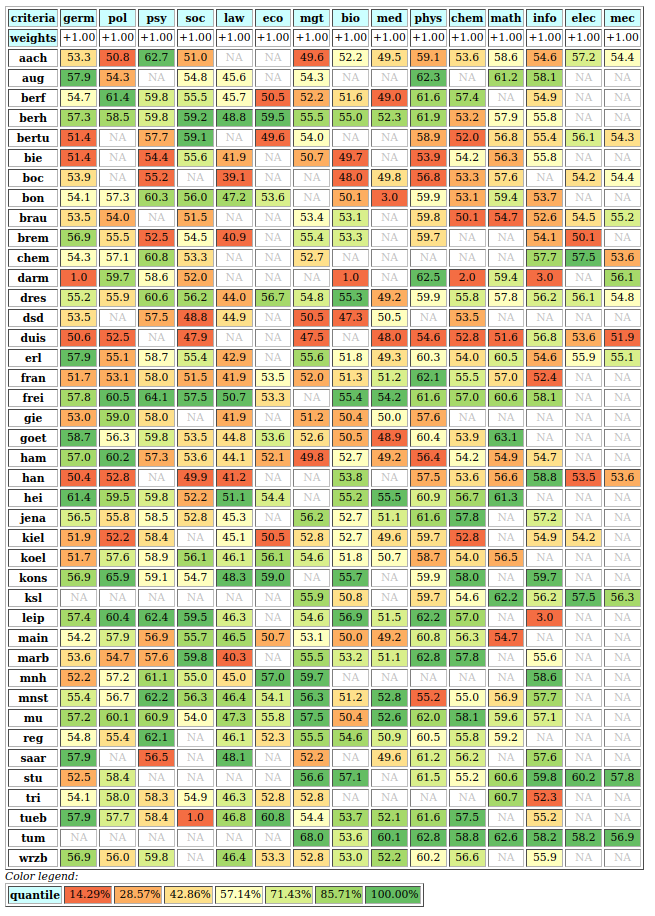
\includegraphics[width=\hsize]{Figures/14-1-ratingData.png}
\caption{Average quality of enrolled students per academic subject}
\label{fig:14.1}       % Give a unique label
\end{figure}
%\clearpage

In Fig.~\vref{fig:14.1}, the fifteen popular academic subjects are grouped into topical 'Faculties': - \emph{Humanities}; - \emph{Law, Economics \& Management}; - \emph{Life Sciences \& Medicine}; - \emph{Natural Sciences \& Mathematics}; and - \emph{Technology}. All fifteen subjects are considered equally significant for our rating problem (see Row 2). The recorded average enrolment quality scores appear coloured along a 7-tiling scheme per subject (see last Row).

We may by the way notice that TU Dresden is the only Institution showing enrolment quality scores in all the fifteen academic subjects. Whereas, on the one side, TU Muenchen and Kaiserslautern are only graded in \emph{Sciences} and \emph{Technology} subjects. On the other side, Mannheim, is only graded in \emph{Humanities} and \emph{Law, Economics \& Management} studies. Most of the 41 Universities are not graded in \emph{Engineering} studies. We are, hence, facing a large part ($27.3\%$) of irreducible missing data (see Listing~\vref{list:14.1} Line 9).

Details of the enrolment quality criteria (the academic subjects) may be consulted in a browser view (see Fig.~\vref{fig:14.2} below).
\begin{lstlisting}
>>> t.showHTMLCriteria()
\end{lstlisting}
 \begin{figure}[h]
%\sidecaption
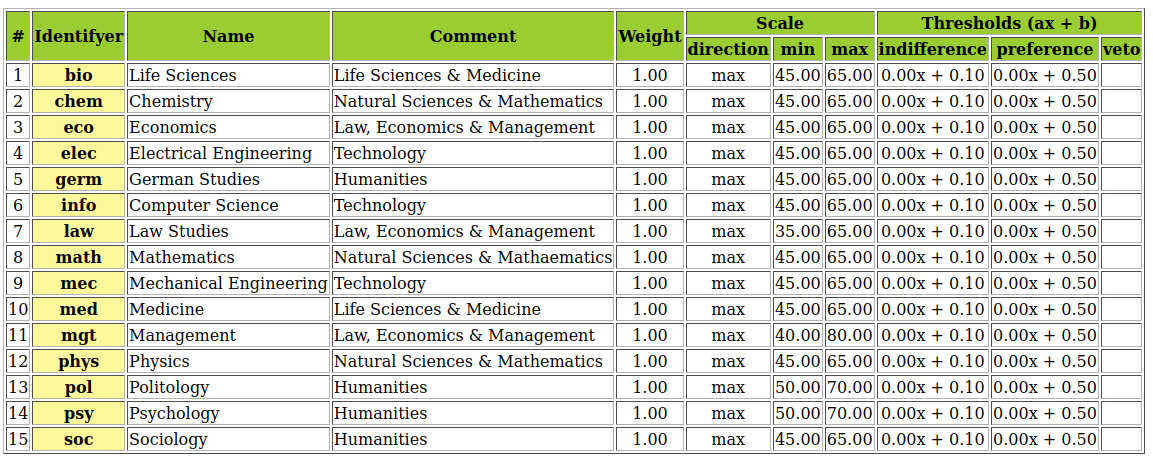
\includegraphics[width=\hsize]{Figures/14-2-spiegelCriteria.png}
\caption{Details of the rating criteria}
\label{fig:14.2}       % Give a unique label
\end{figure}
%\clearpage

The evaluation of the individual quality score for a participating student actually depends on his or her mainly enrolled subject \footnote{The methology (in German) guiding the \emph{Spiegel} survey may be consulted in the \texttt{examples} directory of the \Digraph resources \citep{SPI-2004m}.}. The apparent quality measurement scales thus largely differ indeed from subject to subject (see Fig.~\vref{fig:14.2}), like \emph{Law Studies} ($35.0 - 65-0$) and \emph{Politology} ($50.0 - 70.0$). The recorded average enrolment quality scores, hence, are in fact \emph{incommensurable} between the subjects.

To take furthermore into account a potential and very likely imprecision of the individual quality scores' computation, we shall assume that, for all subjects, an average enrolment quality score difference of $0.1$ is \emph{insignificant}, wheras a difference of $0.5$ is sufficient to positively attest a \emph{better} enrolment quality.

The apparent incommensurability and very likely imprecision of the recorded average enrolment quality scores, renders meaningless any global averaging over the subjects per University of the enrolment quality. We shall therefore, similarly to the methodological approach of the \emph{Spiegel} authors, proceed with an \emph{order statistics} based rating-by-ranking approach (see Chapter~\vref{sec:10} on rating with learned quantile norms).

\section{Rating-by-ranking with lower-closed quantile limits}
\label{sec:14.1}

The \emph{Spiegel} authors opted indeed for a simple 3-tiling of the Universities per valuated academic subject, followed by an average \Borda scores based global ranking. Here, our epistemic logic based outranking approach, allows us, with adequate choices of \emph{indifference} ($0.1$) and \emph{preference} ($0.5$) discrimination thresholds, to estimate \emph{lower-closed} 9-tiles of the enrolment quality scores per subject and rank conjointly, with the help of the \Copeland ranking rule Footnote[34] applied to a corresponding bipolar-valued outranking digraph, the 41 Universities \textbf{and} the lower limits of the estimated 9-tiles limits.

We therefore need in Listing~\vref{list:14.2}, first, to import from the \texttt{performanceQuantiles} module\index{performanceQuantiles@\texttt{performanceQuantiles} module} the \texttt{PerformanceQuantiles} class constructor \index{PerformanceQuantiles@\texttt{PerformanceQuantiles} class} and estimate the lowerclosed 9-tiling of the average enrolment quality scores per academic subject.
\begin{lstlisting}[caption={Computing 9-tiles of the enrolment quality scores per subject},label=list:14.2]
>>> from performanceQuantiles import PerformanceQuantiles
>>> pq = PerformanceQuantiles(t,numberOfBins=9,LowerClosed=True)
>>> pq
  *------- PerformanceQuantiles instance description ------*
    Instance class   : PerformanceQuantiles
    Instance name    : 9-tiled_performances
    Criteria         : 15
    Quantiles        : 9 (LowerClosed)
    History sizes    : {
      'germ': 39, 'pol': 34, 'psy': 34, 'soc': 32,
      'law': 32, 'eco': 21, 'mgt': 34,
      'bio': 34, 'med': 28, 'phys': 37, 'chem': 35, 'math': 27,
      'info': 33, 'elec': 14, 'mec': 13,}
\end{lstlisting}

The history sizes, reported in Listing~\vref{list:14.2} above, indicate the number of Universities graded in each one of the popular fifteen subjects. \emph{German Studies}, for instance, are graded for 39 out of 41 Universities, whereas \emph{Electrical} and \emph{Mechanical Engineering} are only graded for 14, respectively 13 Institutions. None of the fifteen subjects are graded in all the 41 Universities \footnote{It would have been interesting to estimate such quantile limits from the individual qualitiy scores of all the nearly 50,000 surveyed students. But this data was not available \citep{SPI-2004}.}. 

We may inspect the resulting 9-tiling limits in a browser view.
\begin{lstlisting}
>>> pq.showHTMLLimitingQuantiles(Transposed=True,Sorted=False,\
...	   ndigits=1,title='9-tiled quality score limits')
\end{lstlisting}

\begin{figure}[h]
\sidecaption[t]
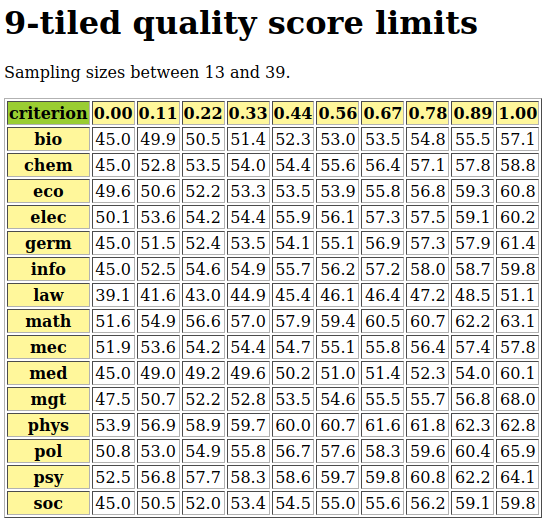
\includegraphics[width=7cm]{Figures/14-3-score9Limits.png}
\caption{9-tiling quality score limits per academic subject. We see confirmed again the incommensurability between the subjects, we noticed already in the apparent enrolment quality scoring , especially between \emph{Law Studies} ($39.1 - 51.1$) and \emph{Politology} ($50.5 - 65.9$). Universities valuated in \emph{Law studies} but not in \emph{Politology}, like the University of Bielefeld, would see their enrolment quality unfairly weakened when simply averaging the enrolment quality scores over valuated subjects}
\label{fig:14.3}       % Give a unique label
\end{figure}
%\clearpage
We add, now, these 9-tiling quality score limits to the enrolment quality records of the 41 Universities and rank, by using the \Copeland rule, all these records conjointly together with the help of the \texttt{LearnedQuantilesRatingDigraph} class\index{LearnedQuantilesRatingDigraph@\texttt{LearnedQuantilesRatingDigraph} class} from the \texttt{sortingDigraphs} module\index{sortingDigraphs@\texttt{sortingDigraphs} module}.
\begin{lstlisting}
>>> from sortingDigraphs import\
...                 LearnedQuantilesRatingDigraph
>>> lqr = LearnedQuantilesRatingDigraph(pq,t,\
...                 rankingRule='Copeland')
\end{lstlisting}

The resulting ranking of the 41 Universities including the lower-closed 9-tiling score limits may be nicely illustrated  with the help of a corresponding heatmap view . 
\begin{lstlisting}
>>> lqr.showHTMLRatingHeatmap(colorLevels=7,\
...              Correlations=True,\
...              ndigits=1,rankingRule='Copeland')
\end{lstlisting}
\begin{figure}[h]
%\sidecaption
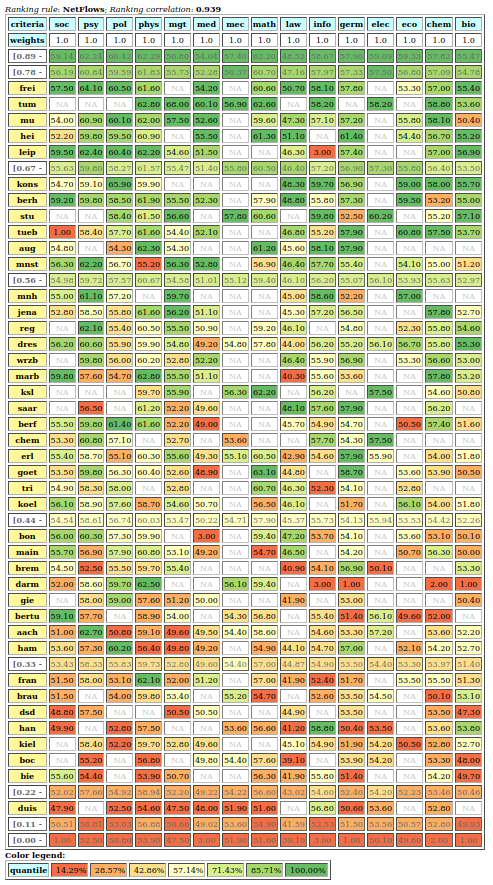
\includegraphics[width=\hsize]{Figures/14-4-nineTilingResult.png}
\caption{Heatmap view of the 9-tiles rating-by-ranking result}
\label{fig:14.4}       % Give a unique label
\end{figure}
%\clearpage

The ordinal correlation ($+0.967$) of the \Copeland ranking with the underlying bipolar-valued outranking digraph is very high (see Fig.~\vref{fig:14.4} Row 1). Most correlated subjects with this rating-by-ranking result appear to be \emph{German Studies} ($+0.51$), \emph{Chemistry} ($+0.48$), \emph{Management} ($+0.47$) and \emph{Physics} ($+0.46$). Both \emph{Electrical} ($+0.07$) and \emph{Mechanical Engineering} ($+0.05$) are the less correlated subjects (see Row 3).

From the actual ranking position of the lower 9-tiling limits, we may now immediately deduce the 9-tile enrolment quality equivalence classes. No University reaches the highest 9-tile ($[0.89 - [$). In the lowest 9-tile ($[0.00- 0.11]$) we find the University Duisburg. The complete rating result may be easily printed out as follows with the \texttt{showQuantilesRating()} method\index{showQuantilesRating@\texttt{showQuantilesRating()}}:
\begin{lstlisting}[caption={Showing the 9-tiling of the enrolment quality of the 41 Universities},label=list:14.3]
>>> lqr.showQuantilesRating()
    *-------- Quantiles rating result ---------
     [0.89 - 1.00] []
     [0.78 - 0.89[ ['tum','frei','kons','leip','mu','hei']
     [0.67 - 0.78[ ['stu','berh']
     [0.56 - 0.67[ ['aug','mnh','tueb','mnst','jena',
                    'reg','saar']
     [0.44 - 0.56[ ['wrzb','dres','ksl','marb','berf',
                    'chem','koel','erl','tri']
     [0.33 - 0.44[ ['goet','main','bon','brem']
     [0.22 - 0.33[ ['fran','ham','kiel','aach',
                    'bertu','brau','darm']
     [0.11 - 0.22[ ['gie','dsd','bie','boc','han']
     [0.00 - 0.11[ ['duis']
\end{lstlisting}

Following Universities: TU München, Freiburg, Konstanz, Leipzig, München as well as Heidelberg, appear best rated in the eigth 9-tile ($[0.78 - 0.89[$, see Listing~\vref{list:14.3} Line 4). Lowest-rated in the first 9-tile, as mentioned before, appears University Duisburg (Line 14). Midfield, the fifth 9-tile ($[0.44 - 0.56[$), consists of the Universities Würzburg, TU Dresden, Kaiserslautern, Marburg, FU Berlin, Chemnitz, Köln , Erlangen-Nürnberg and Trier (Lines 8-9).

A corresponding \emph{graphviz} drawing may well illustrate all these enrolment quality equivalence classes.
\begin{lstlisting}
>>> lqr.exportRatingByRankingGraphViz(fileName='ratingResult',\
...                                   graphSize='12,12')
  *---- exporting a dot file for GraphViz tools ---------*
   Exporting to ratingResult.dot
   dot -Grankdir=TB -Tpdf dot -o ratingResult.png
\end{lstlisting}
\begin{figure}[ht]
%\sidecaption
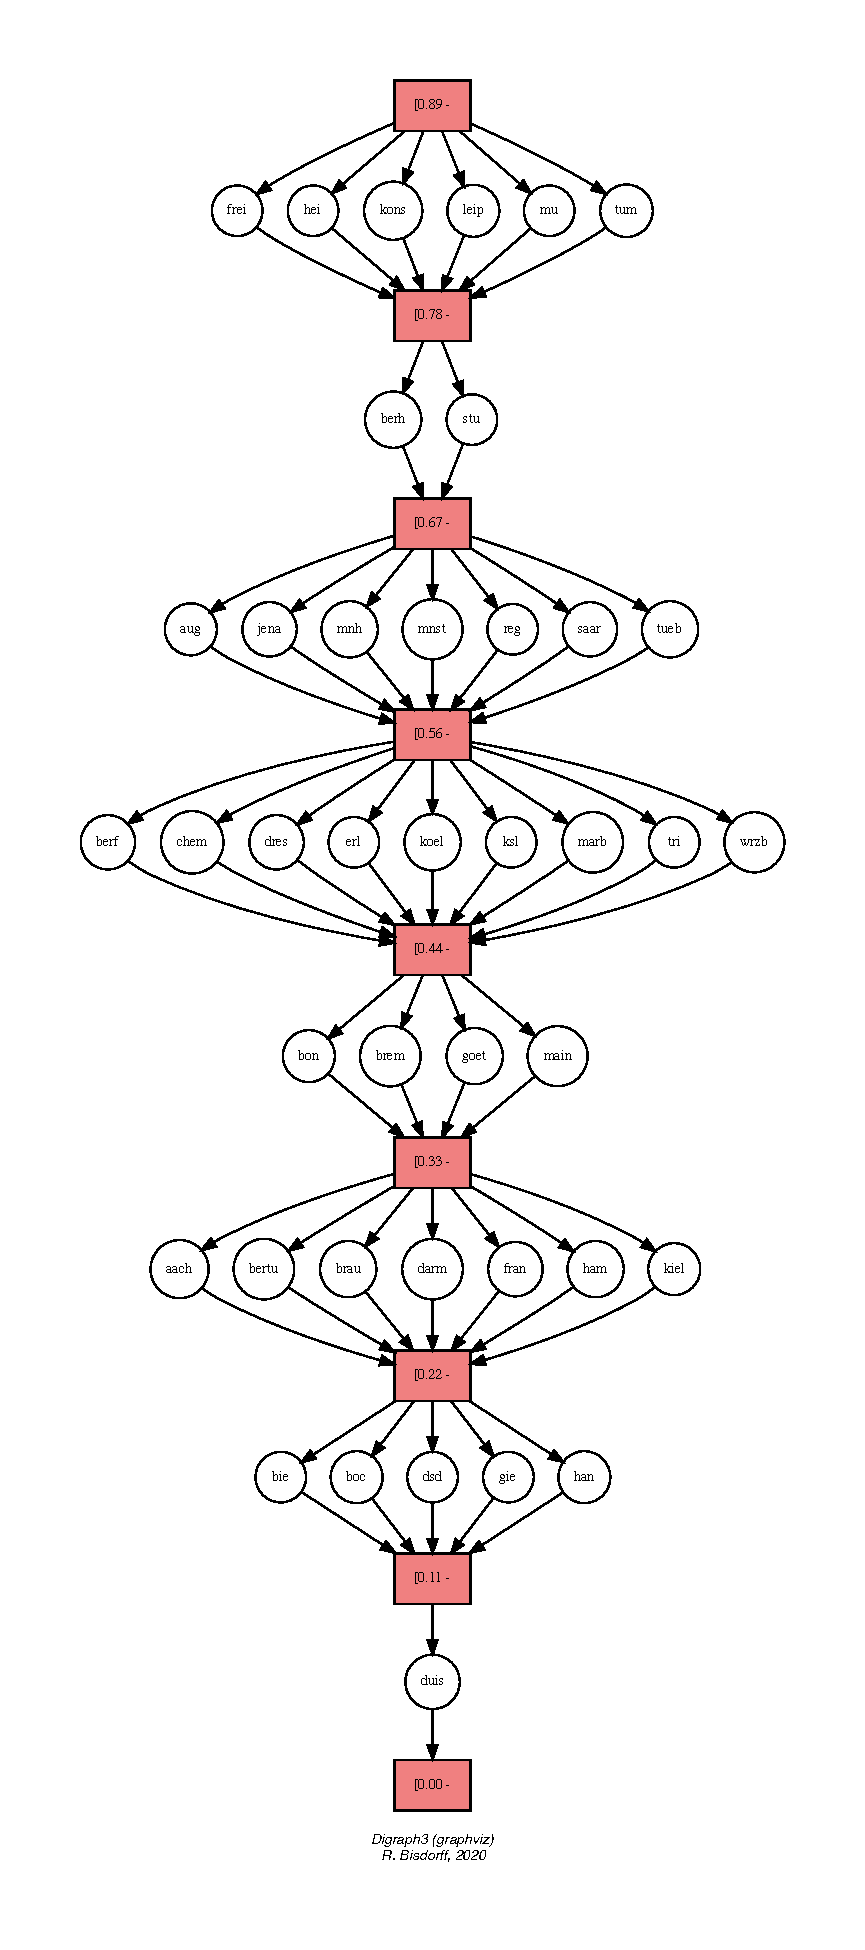
\includegraphics[height=0.9\vsize]{Figures/14-5-ratingResult.pdf}
\caption{Drawing of the 9-tiles rating-by-ranking result}
\label{fig:14.5}       % Give a unique label
\end{figure}

We have noticed in Chapter~\vref{sec:8}, that there is not a single optimal rule for ranking from a given outranking digraph. The \Copeland rule, for instance, has the advantage of being \Condorcet consistent, i.e. when the outranking digraph models in fact a linear ranking, this ranking will necessarily be the result of the \Copeland* rule. When this is not the case, and especially when the outranking digraph shows many circuits, all potential ranking rules may give very divergent ranking results, and hence also substantially divergent rating-by-ranking results.

It is, hence, interesting, to verify if the epistemic fusion of the rating-by-ranking results, one may obtain when applying two different ranking rules, like the \Copeland and the \NetFlows ranking rule, does actually confirm our rating-by-ranking result shown in Fig.~\vref{fig:14.5}. For this purpose we make usage of the \texttt{RankingsFusionDigraph} constructor\index{RankingsFusionDigraph@\texttt{RankingsFusionDigraph} class} (see Line 9 below).
\begin{lstlisting}
>>> lqr = LearnedQuantilesRatingDigraph(\
...                   pq,t,rankingRule='Copeland')
>>> lqr1 = LearnedQuantilesRatingDigraph(\
...                   pq,t,rankingRule='NetFlows')
>>> from transitiveDigraphs import\
...                RankingsFusionDigraph
>>> rankings = [lqr.actionsRanking, lqr1.actionsRanking]
>>> rf = RankingsFusionDigraph(lqr,rankings)
>>> rf.exportGraphViz(fileName='fusionResult',\
...           WithRatingDecoration=True,\
...           graphSize='30,30')
  exporting a dot file for GraphViz tools
   Exporting to fusionResult.dot
   dot -Grankdir=TB -Tpng fusionResult.dot\
...                  -o fusionResult.png
\end{lstlisting}
\begin{figure}[h]
\sidecaption[t]
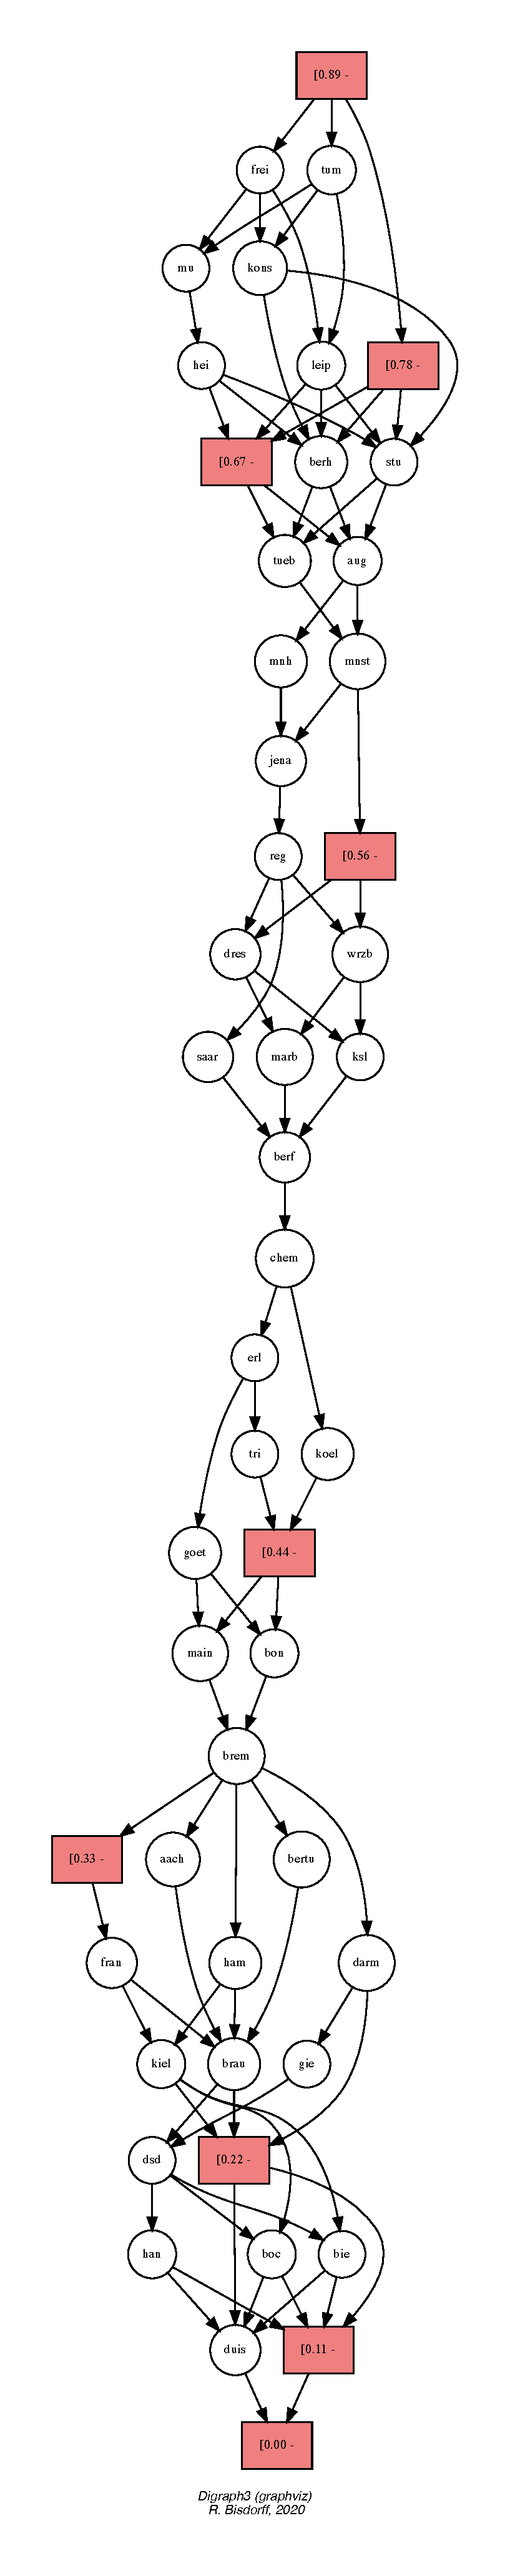
\includegraphics[height=0.9\vsize]{Figures/14-6-fusionResult.pdf}
\caption{Disjunctive fusion of the \Copeland and the \NetFlows rankings (extract).}
\label{fig:14.6}       % Give a unique label
\end{figure}

In Fig.~\vref{fig:14.6} we notice that many Universities appear now rated into several adjacent 9-tiles. The previously best-rated Universities: TU München, Freiburg, München, Leipzig, as well as  Heidelberg, for instance, appear now sorted into the $7^{th}$ and $8^{th}$ 9-tile ($[0.67 - 0.89]$), whereas Konstanz is now, even more imprecisely, rated into the $6^{th}$, the $7^{th}$ and the $8^{th}$ 9-tile.
How confident, hence, is our precise \Copeland rating-by-ranking result? To investigate this question, let us now inspect the outranking digraph on which we actually apply the \Copeland ranking rule.

\section{Inspecting the bipolar-valued outranking digraph}
\label{sec:14.2}

We say that University x \emph{outranks} (resp. \emph{is outranked by}) University $y$ in enrolment quality when there exists a majority (resp. only a minority) of valuated subjects showing an \emph{at least as good as} average enrolment quality score. To compute these outranking situations, we use the \texttt{BipolarOutrankingDigraph} constructor.
\begin{lstlisting}[caption={Computing 9-tiles of the enrolment quality scores per subject},label=list:14.4]
>>> from outrankingDigraphs import BipolarOutrankingDigraph
>>> dg = BipolarOutrankingDigraph(t) 
>>> dg
  *------- Object instance description ------*
    Instance class       : BipolarOutrankingDigraph
    Instance name        : rel_studentenSpiegel04
    Actions              : 41 (Universities)
    Criteria             : 15 (subjects)
    Size                 : 828 (outranking situations)
    Determinateness (%)  : 63.67
    Valuation domain     : [-1.00;1.00]
>>> dg.computeTransitivityDegree(Comments=True)
    Transitivity degree of digraph <rel_studentenSpiegel04>:
     triples x>y>z: 57837, closed: 30714, open: 27123
     (closed/triples) =  0.531
>>> dg.computeSymmetryDegree(Comments=True)
    Symmetry degree of digraph <rel_studentenSpiegel04>:
     arcs x>y: 793, symmetric: 35, asymmetric: 758
     symmetric/arcs =  0.044
\end{lstlisting}

The bipolar-valued outranking digraph $dg$ (see Listing~\vref{list:14.4} Line 2), obtained with the given performance tableau $t$, shows 828 positively validated pairwise outranking situations (Line 9). Unfortunately, the transitivity of digraph $dg$ is far from being satisfied: nearly half of the transitive closure is missing (Line 15). Despite the rather large preference discrimination threshold (0.5) we have assumed (see Fig.~\vref{fig:14.2}), there does not occur many indifference situations (Line 19).

We may furthermore check if there exists any \emph{cyclic} outranking situations.
\begin{lstlisting}[caption={Enumerating chordless outranking circuits},label=list:14.5]
>>> from outrankingDigraphs import BipolarOutrankingDigraph
>>> dg.computeChordlessCircuits()
>>> dg.showChordlessCircuits()
  *---- Chordless circuits ----*
   93 circuits.
    1:  ['aach','bie','darm','brau'] ,credibility : 0.067
    2:  ['aach','bertu','brau'] ,credibility : 0.200
    3:  ['aach','bertu','brem'] ,credibility : 0.067
    4:  ['aach','bertu','ham'] ,credibility : 0.200
    5:  ['aug','tri','marb'] ,credibility : 0.067
    6:  ['aug','jena','marb'] ,credibility : 0.067
    7:  ['aug','jena','koel'] ,credibility : 0.067
     ...
     ...
   29:  ['berh','kons','mu'] ,credibility : 0.133
     ...
     ...
   88:  ['main','mnh','marb'] ,credibility : 0.067
   89:  ['marb','saar','wrzb'] ,credibility : 0.067
   90:  ['marb','saar','reg'] ,credibility : 0.067
   91:  ['marb','saar','mnst'] ,credibility : 0.133
   92:  ['marb','saar','tri'] ,credibility : 0.067
   93:  ['mnh','mu','stu'] ,credibility : 0.133
 \end{lstlisting}
Here we observe indeed 93 such outranking circuits, like: Berlin Humboldt $>$ Konstanz $>$ München $>$ Berlin Humboldt, supported by a $(0.133 + 1.0)/2 = 56.7\%$ majority of subjects Footnote[31] (see circuit 29 above). In the \Copeland ranking result shown in Fig.~\vref{fig:14.4}, these Universities appear positioned respectively at ranks 10, 4 and 6. In the \NetFlows ranking result they would appear respectively at ranks 10, 6 and 5, thus inverting the positions of Konstanz and München. The occurrence in digraph $dg$ of so many outranking circuits makes thus \emph{doubtful} any \emph{forced} linear ranking, independently of the specific ranking rule we might have applied.

To effectively check the quality of our \Copeland rating-by-ranking result, we shall now compute a direct sorting into 9-tiles of the enrolment quality scores, without using any outranking digraph based ranking rule.

\section{Rating by quantiles sorting}
\label{sec:14.3}

In our case here, the Universities represent the decision actions: \emph{where to study}. We say now that University $x$ is sorted into the lower-closed 9-tile $q$ when the performance record of $x$ positively outranks the lower limit record of 9-tile $q$ and $x$ does not positively outrank the upper limit record of 9-tile $q$. 

\begin{lstlisting}[caption={Enumerating chordless outranking circuits},label=list:14.6,basicstyle=\ttfamily\scriptsize]
>>> lqr.showActionsSortingResult()
  Quantiles sorting result per decision action
  [0.33 - 0.44[: aach with credibility: 0.13 = min(0.13,0.27)
  [0.56 - 0.89[: aug with credibility: 0.13 = min(0.13,0.27)
  [0.44 - 0.67[: berf with credibility: 0.13 = min(0.13,0.20)
  [0.78 - 0.89[: berh with credibility: 0.13 = min(0.13,0.33)
  [0.22 - 0.44[: bertu with credibility: 0.20 = min(0.33,0.20)
  [0.11 - 0.22[: bie with credibility: 0.20 = min(0.33,0.20)
  [0.22 - 0.33[: boc with credibility: 0.07 = min(0.07,0.07)
  [0.44 - 0.56[: bon with credibility: 0.13 = min(0.20,0.13)
  [0.33 - 0.44[: brau with credibility: 0.07 = min(0.07,0.27)
  [0.33 - 0.44[: brem with credibility: 0.07 = min(0.07,0.07)
  [0.44 - 0.56[: chem with credibility: 0.07 = min(0.13,0.07)
  [0.22 - 0.56[: darm with credibility: 0.13 = min(0.13,0.13)
  [0.56 - 0.67[: dres with credibility: 0.27 = min(0.27,0.47)
  [0.22 - 0.33[: dsd with credibility: 0.07 = min(0.07,0.07)
  [0.00 - 0.11[: duis with credibility: 0.33 = min(0.73,0.33)
  [0.44 - 0.56[: erl with credibility: 0.13 = min(0.27,0.13)
  [0.22 - 0.44[: fran with credibility: 0.13 = min(0.13,0.33)
  [0.78 - <[: frei with credibility: 0.53 = min(0.53,1.00)
  [0.22 - 0.33[: gie with credibility: 0.13 = min(0.13,0.20)
  [0.33 - 0.44[: goet with credibility: 0.07 = min(0.47,0.07)
  [0.22 - 0.33[: ham with credibility: 0.07 = min(0.33,0.07)
  [0.11 - 0.22[: han with credibility: 0.20 = min(0.33,0.20)
  [0.78 - 0.89[: hei with credibility: 0.13 = min(0.13,0.27)
  [0.56 - 0.67[: jena with credibility: 0.07 = min(0.13,0.07)
  [0.33 - 0.44[: kiel with credibility: 0.20 = min(0.20,0.47)
  [0.44 - 0.56[: koel with credibility: 0.07 = min(0.27,0.07)
  [0.78 - <[: kons with credibility: 0.20 = min(0.20,1.00)
  [0.56 - 0.89[: ksl with credibility: 0.13 = min(0.13,0.40)
  [0.78 - 0.89[: leip with credibility: 0.07 = min(0.20,0.07)
  [0.44 - 0.56[: main with credibility: 0.07 = min(0.07,0.13)
  [0.56 - 0.67[: marb with credibility: 0.07 = min(0.07,0.07)
  [0.56 - 0.89[: mnh with credibility: 0.20 = min(0.20,0.27)
  [0.56 - 0.67[: mnst with credibility: 0.07 = min(0.20,0.07)
  [0.78 - 0.89[: mu with credibility: 0.13 = min(0.13,0.47)
  [0.56 - 0.67[: reg with credibility: 0.20 = min(0.20,0.27)
  [0.56 - 0.78[: saar with credibility: 0.13 = min(0.13,0.20)
  [0.78 - 0.89[: stu with credibility: 0.07 = min(0.13,0.07)
  [0.44 - 0.56[: tri with credibility: 0.07 = min(0.13,0.07)
  [0.67 - 0.78[: tueb with credibility: 0.13 = min(0.13,0.20)
  [0.89 - <[: tum with credibility: 0.13 = min(0.13,1.00)
  [0.56 - 0.67[: wrzb with credibility: 0.07 = min(0.20,0.07)
\end{lstlisting}
In the 9-tiles sorting result, shown in Listing~\vref{list:14.6}, we notice for instance in Lines 3-4 that the RWTH Aachen is precisely rated into the 4th 9-tile ($[0.33 - 0.44[$), whereas the University Augsburg is less precisely rated conjointly into the $6^{th}$, the $7^{th}$ and the $8^{th}$ 9-tile ($[0.56 - 0.89[$). In Line 42, TU München appears best rated into the unique highest 9-tile ($[0.89 - <[$). All three rating results are supported by a $(0.07 + 1.0)/2 = 53.5\%$ majority of valuated subjects \footnote{Converted by a $+1.0$ shift and a $0.5 \times 100$ scale transform from a bipolar-valued credibility of $+0.07$ in $[-1.0, +1.0]$ to a majority (in \%) support.}. With the support of a $76.5\%$ majority of valuated subjects (Line 20), the apparent most confident rating result is the one of University Freiburg (see also Fig.~\vref{fig:14.3} and Fig.~\vref{fig:14.4}). 

We shall now lexicographically sort these individual rating results per University, by \emph{average} rated 9-tile limits and highest-rated upper 9-tile limit, into ordered, but not necessarily disjoint, enrolment quality quantiles.
\begin{lstlisting}
>>> lqr.showHTMLQuantilesSorting(strategy='average')
\end{lstlisting}
\begin{figure}[h]
\sidecaption[t]
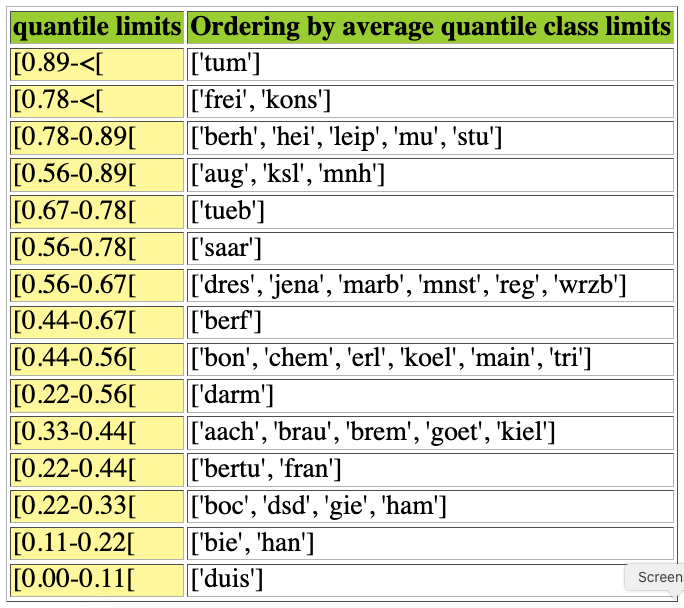
\includegraphics[width=6cm]{Figures/14-7-nineTilingOrdering.png}
\caption{The ranked 9-tiles rating-by-sorting result. We may notice that the Universities: Augsburg, Kaiserslautern, Mannheim and Tübingen, for instance, show in fact the same average rated 9-tiles score of $0.725$; yet, the rated upper 9-tile limit of Tuebingen reaches only $0.78$, whereas the one of the other Universities reaches $0.89$. Hence, Tuebingen is ranked below Augsburg, Kaiserslautern and Mannheim}
\label{fig:14.7}       % Give a unique label
\end{figure}

With a special \emph{graphviz} drawing of the \texttt{LearnedQuantilesRatingDigraph} instance $lqr$, we may, without requiring any specific ordering strategy, as well illustrate our 9-tiles rating-by-sorting result.
\begin{lstlisting}
>>> lqr.exportRatingBySortingGraphViz(\
...           'nineTilingDrawing',graphSize='12,12')
  *---- exporting a dot file for GraphViz tools --*
   Exporting to nineTilingDrawing.dot
   dot -Grankdir=TB -Tpng nineTilingDrawing.dot\
                     -o nineTilingDrawing.png
\end{lstlisting}
\begin{figure}[ht]
%\sidecaption
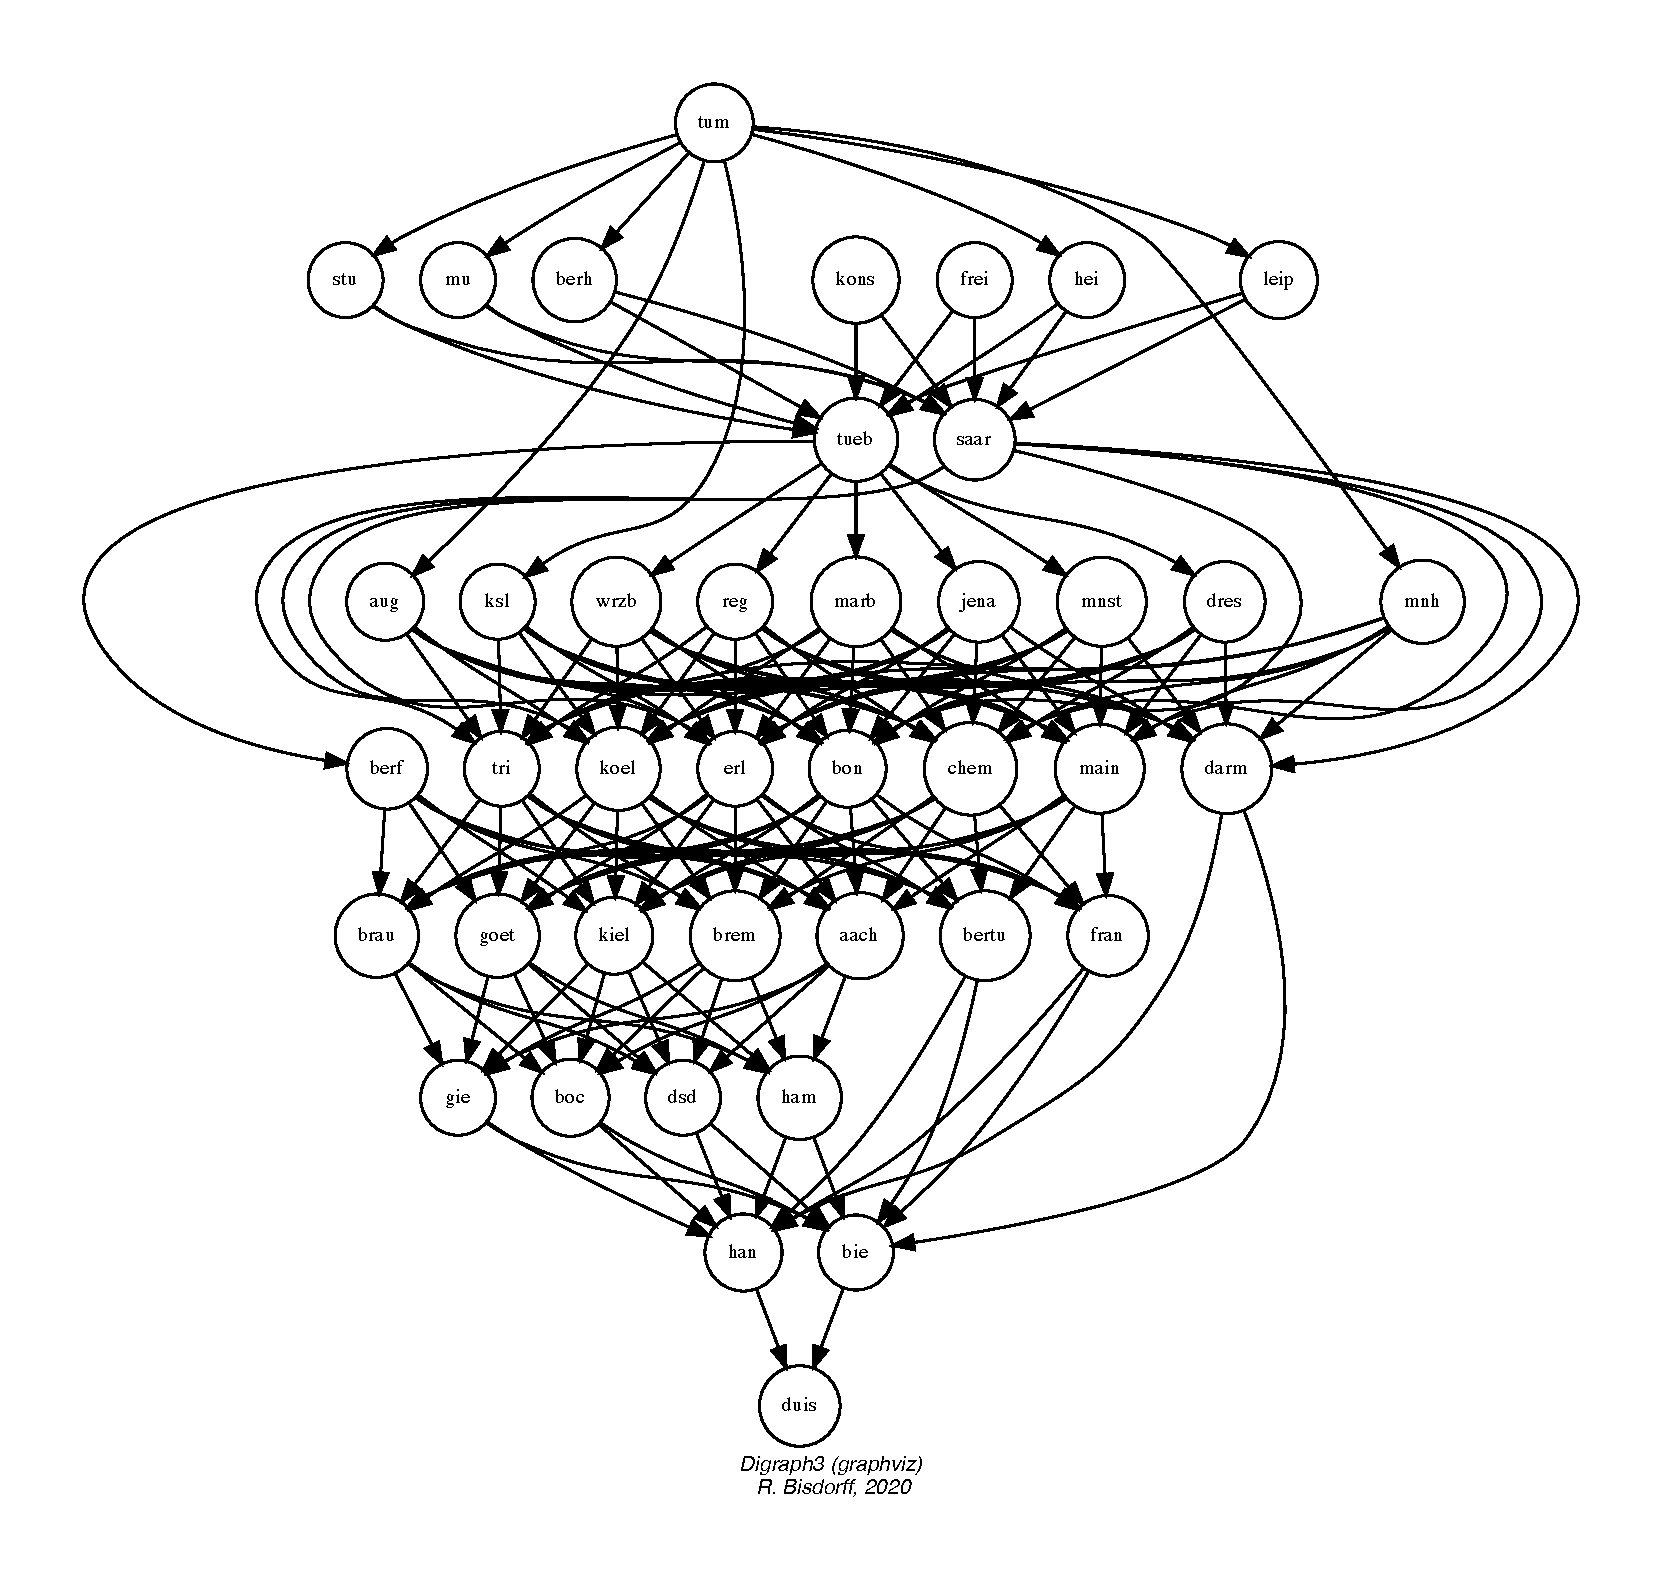
\includegraphics[width=\hsize]{Figures/14-8-nineTilingDrawing.pdf}
\caption{Graphviz drawing of the 9-tiles sorting digraph.}
\label{fig:14.8}       % Give a unique label
\end{figure}
%\clearpage

In Fig.~\vref{fig:14.8} we actually see the \emph{skeleton} (transitive closure removed) of a partial order, where an oriented arc is drawn between Universities x and y when their 9-tiles sorting results are disjoint and the one of x is higher rated than the one of $y$. The rating for TU München (see Listing~\vref{list:14.6} Lines 45), for instance, is disjoint and higher rated than the one of the Universities Freiburg and Konstanz (Lines 23, 32). And, both the ratings of Feiburg and Konstanz are, however, not disjoint from the one, for instance, of the Universty of Stuttgart (Line 42).

The partial ranking, shown in Fig.~\vref{fig:14.8}, is in fact independent of any ordering strategy: - \emph{average}, - \emph{optimistic} - \emph{pessimistic}, of overlapping 9-tiles sorting results, and confirms that the same Universities as with the previous rating-by-ranking approach, namely TU München, Freiburg, Konstanz, Stuttgart, Berlin Humboldt, Heidelberg and Leipzig appear top-rated. Similarly, the Universities of Duisburg, Bielefeld, Hanover, Bochum, Giessen, Düsseldorf and Hamburg give the lowest-rated group. The midfield here is again consisting of more or less the same Universities as the one observed in the previous rating-by-ranking approach (see Listing~\vref{list:14.3}).

In the end, both the \Copeland rating-by-ranking, as well as the rating-by-sorting approach give luckily, in our case study here, very similar results. The first approach, with its \emph{forced} linear ranking, determines on the one hand, precise enrolment quality equivalence classes; a result, depending potentially a lot on the actually applied ranking rule. The rating-by-sorting approach, on the other hand, only determines for each University a less precise but prudent rating of its individual enrolment quality, furthermore supported by a known majority of performance criteria significance; a somehow fairer and robuster result, but, much less evident for easily comparing the apparent enrolment quality among Universities. Contradictorily, or sparsely valuated Universities, for instance, will appear trivially rated into a large midfield of adjacent 9-tiles.

Let us conclude by saying that we prefer this latter rating-by-sorting approach; perhaps impreciser, due the case given, to missing and contradictory performance data; yet, well grounded in a powerful bipolar-valued logical and espistemic framework.
 
%%%%%%% The chapter bibliography
%\normallatexbib
\clearpage
%\phantomsection
%\addcontentsline{toc}{section}{Chapter Bibliography}
\bibliographystyle{spbasic}
%\typeout{}
\bibliography{03-backMatters/reference}
%\chapter{The best academic Computer Science Depts: A ranking case study}
\label{sec:13}

\abstract*{ In this case study, we are solving with our \Digraph resources a ranking decision problem based on published data from the \emph{Times Higher Education} (THE) \emph{World University Rankings} 2016 by \emph{Computer Science} (CS) subject. Several hundred academic CS Departments, from all over the world, were ranked that year following an overall numerical score based on the weighted average of five performance criteria: \emph{Teaching} (the learning environment, $30\%$), \emph{Research} (volume, income and reputation, $30\%$), \emph{Citations} (research influence, $27.5\%$), \emph{International outlook} (staff, students, and research, $7.5\%$), and \emph{Industry income} (innovation, $5\%$). To illustrate our \Digraph programming resources, we shall first have a look into the THE ranking data with short Python scripts. In a second section, we shall relax the commensurability hypothesis of the ranking criteria and show how to similarly rank with multiple incommensurable performance criteria of solely ordinal significance. A third Section is finally devoted to introduce quality measures for qualifying ranking results.}

\abstract{ In this case study, we are solving with our \Digraph resources a ranking decision problem based on published data from the \emph{Times Higher Education} (THE) \emph{World University Rankings} 2016 by \emph{Computer Science} (CS) subject. Several hundred academic CS Departments, from all over the world, were ranked that year following an overall numerical score based on the weighted average of five performance criteria: \emph{Teaching} (the learning environment, $30\%$), \emph{Research} (volume, income and reputation, $30\%$), \emph{Citations} (research influence, $27.5\%$), \emph{International outlook} (staff, students, and research, $7.5\%$), and \emph{Industry income} (innovation, $5\%$). To illustrate our \Digraph programming resources, we shall first have a look into the THE multiple-criteria ranking data with short Python scripts. In a second section, we shall relax the commensurability hypothesis of the ranking criteria and show how to similarly rank with multiple incommensurable performance criteria of solely ordinal significance. A third section is finally devoted to introduce quality measures for qualifying ranking results.
}

\section{The THE performance tableau}
\label{sec:13.1}

For this decision making case study, we use an extract of the published \THE (THE) World University rankings 2016 by Computer Science (CS) subject, concerning the 75 first-ranked academic Institutions\footnote{\href{https://www.timeshighereducation.com/world-university-rankings/2017/subject-ranking/computer-science}{THE World University Rankings 2016 by Computer Science subject}}. The multiple-criteria performance tableau data, collected from the THE web pages, is stored in a file named \texttt{the-cs-2016.py} of \texttt{PerformanceTableau} format \footnote{The performance tableau \texttt{the-cs-2016.py} is available in the \texttt{examples} directory of the \Digraph resources \citep{BIS-2021}.}.\index{THE University rankings 2016 by CS subject} 
\begin{lstlisting}[caption={Performance tableau of the },label=list:13.1]
>>> from perfTabs import PerformanceTableau
>>> cspt = PerformanceTableau('the_cs_2016')
>>> cspt
  *------- PerformanceTableau instance description ------*
   Instance class     : PerformanceTableau
   Instance name      : the-cs-2016
   Actions            : 75
   Objectives         : 5
   Criteria           : 5
   NaN proportion (%) : 0.0
   Attributes         : ['name','description','actions',
                           'objectives','criteria',
			   'weightPreorder','NA','evaluation']
\end{lstlisting}

Potential decision alternatives, in our case here, are the 75 THE best-ranked CS Departments in 2016, all of them located at world renowned Institutions, like California Institute of Technology, Swiss Federal Institute of Technology Zurich, Technical University München, University of Oxford or the National University of Singapore (see List.~\vref{list:13.2} below). 

Instead of using prefigured \Digraph \texttt{show...()} methods, readily available for inspecting \texttt{PerformanceTableau} instances, Listing~\vref{list:13.2} illustrates how to write small Python scripts for printing out its content.   
\begin{lstlisting}[caption={Printing the CS Departments},label=list:13.2,basicstyle=\ttfamily\scriptsize]
>>> for x in cspt.actions:
...     print('%s:\t%s (%s)' %\
...        (x,cspt.actions[x]['name'],cspt.actions[x]['comment']) )
  albt:	University of Alberta (CA)
  anu:	Australian National University (AU)
  ariz:	Arizona State University (US)
  bju:	Beijing University (CN)
  bro:	Brown University (US)
  calt:	California Institute of Technology (US)
  cbu:	Columbia University (US)
  chku:	Chinese University of Hong Kong (HK)
  cihk:	City University of Hong Kong (HK)
  cir:	University of California at Irvine (US)
  cmel:	Carnegie Mellon University (US)
  cou:	Cornell University (US)
  csb:	University of California at Santa Barbara (US)
  csd:	University Of California at San Diego (US)
  dut:	Delft University of Technology (NL)
  eind:	Eindhoven University of Technology (NL)
  ens:	Superior Normal School at Paris (FR)
  epfl:	Swiss Federal Institute of Technology Lausanne (CH)
  epfr:	Polytechnic school of Paris (FR)
  ethz:	Swiss Federal Institute of Technology Zurich (CH)
  frei:	University of Freiburg (DE)
  git:	Georgia Institute of Technology (US)
  glas:	University of Glasgow (UK)
  hels:	University of Helsinki (FI)
  hkpu:	Hong Kong Polytechnic University (CN)
  hkst:	Hong Kong University of Science and Technology (HK)
  hku:	Hong Kong University (HK)
  humb:	Berlin Humboldt University (DE)
  icl:	Imperial College London (UK)
  indis:Indian Institute of Science (IN)
  itmo:	ITMO University (RU)
  kcl:	King's College London (UK)
  kist:	Korea Adv. Institute of Science and Technology (KR)
  kit:	Karlsruhe Institute of Technology (DE)
  kth:	KTH Royal Institute of Technology (SE)
  kuj:	Kyoto University (JP)
  kul:	Catholic University Leuven (BE)
  lms:	Lomonosov Moscow State University (RU)
  man:	University of Manchester (UK)
  mcp:	University of Maryland College Park (US)
  mel:	University of Melbourne (AU)
  mil:	Polytechnic University of Milan (IT)
  mit:	Massachusetts Institute of Technology (US)
  naji:	Nanjing University (CN)
  ntu:	Nanyang Technological University of Singapore (SG)
  ntw:	National Taiwan University (TW)
  nyu:	New York University (US)
  oxf:	University of Oxford (UK)
  pud:	Purdue University (US)
  qut:	Queensland University of Technology (AU)
  rcu:	Rice University (US)
  rwth:	RWTH Aachen University (DE)
  shJi:	Shanghai Jiao Tong University (CN)
  sing:	National University of Singapore (SG)
  sou:	University of Southhampton (UK)
  stut:	University of Stuttgart (DE)
  tech:	Technion - Israel Institute of Technology (IL)
  tlavu:Tel Aviv University (IR)
  tsu:	Tsinghua University (CN)
  tub:	Technical University of Berlin (DE)
  tud:	Technical University of Darmstadt (DE)
  tum:	Technical University of Muenchen (DE)
  ucl:	University College London (UK)
  ued:	University of Edinburgh (UK)
  uiu:	University of Illinois at Urbana-Champagne (US)
  unlu:	University of Luxembourg (LU)
  unsw:	University of New South Wales (AU)
  unt:	University of Toronto (CA)
  uta:	University of Texas at Austin (US)
  utj:	University of Tokyo (JP)
  utw:	University of Twente (NL)
  uwa:	University of Waterloo (CA)
  wash:	University of Washington (US)
  wtu:	Vienna University of Technology (AUS)
  zhej:	Zhejiang University (CN)
\end{lstlisting}

The THE authors base their 2016 ranking on five decision objectives \citep{THE-2016}.
\begin{lstlisting}[caption={The THE ranking objectives},label=list:13.3,basicstyle=\ttfamily\scriptsize]
>>> for obj in cspt.objectives:
...     print('%s: %s (%.1f%%),\n\t%s' %\
...                (obj,cspt.objectives[obj]['name'],\
...                 cspt.objectives[obj]['weight'],
...                 cspt.objectives[obj]['comment'])\
...           ) 
 Teaching: Best learning environment (30.0%)
   Reputation survey; Staff-to-student ration;
   Doctorate-to-student ratio;
   Doctorate-to-academic-staff ratio;
   Institutional income.
 Research: Highest volume and reputation (30.0%)
   Reputation survey;
   Research income;
   Research productivity.
 Citations: Highest research influence (27.5%)
   Impact.
 International outlook: Most international staff,
                        students and research (7.5%)
   Proportions of international students;
   Proportions of international staff;
   International collaborations.
 Industry income: Best knowledge transfer (5.0%)
   Volume.
\end{lstlisting}

With a cumulated importance of $87\%$ (see above), \emph{Teaching}, \emph{Research} and \emph{Citations} represent clearly the major ranking objectives. \emph{International outlook} and \emph{Industry income} are considered of minor importance ($12.5\%$).

THE authors do, unfortunately, not publish the detail of their performance assessments for evaluating CS Depts with respect to each one of performance criteria per ranking objective.  \footnote{THE gives some insight on the subject and significance of the actual ranking criteria used for evaluating along each ranking objective on her website \citep{THE-2016}}. The THE 2016 ranking publication reveals solely a compound assessment on a single performance criteria per ranking objective. The five retained performance criteria may be printed out as follows.
\begin{lstlisting}
>>> for g in cspt.criteria:
...     print('%s:\t%s, %s (%.1f%%)' %\
...       (g,cspt.criteria[g]['name'],cspt.criteria[g]['comment'],\
...        cspt.criteria[g]['weight']) )  
  gtch:	Teaching, The learning environment (30.0%)
  gres:	Research, Volume, income and reputation (30.0%)
  gcit:	Citations, Research influence (27.5%)
  gint:	International outlook, In staff, students and research (7.5%)
  gind:	Industry income, knowledge transfer (5.0%)
\end{lstlisting}

The largest part ($87.5\%$) of criteria significance is, hence canonically, allocated to the major ranking criteria: \emph{Teaching} ($30\%$), \emph{Research} ($30\%$) and \emph{Citations} ($27.5\%$). The small remaining part ($12.5\%$) goes to \emph{International outlook} ($7.5\%$) and \emph{Industry income} ($5\%$).

In order to render commensurable these performance criteria, the THE authors replace, per criterion, the actual performance evaluation obtained by each University with the corresponding \emph{quantile} observed in the cumulative distribution of the performance evaluations obtained by all the surveyed institutions \citep{THE-2016}. The THE ranking is eventually determined by an \emph{overall score} per University which corresponds to the weighted average of these five criteria quantiles, as illustrated in Listing~\vref{list:13.4}.     
\begin{lstlisting}[caption={Computing the THE overall scores},label=list:13.4]
>>> theScores = []
>>> for x in cspt.actions:
...     xscore = Decimal('0')
...     for g in cspt.criteria:
...         xscore += cspt.evaluation[g][x] *\
...          (cspt.criteria[g]['weight']/Decimal('100'))
...	   theScores.append((xscore,x))
\end{lstlisting}

In Listing~\vref{list:13.5} (Lines 15-16), we may thus notice that, in the 2016 edition of the THE World University rankings by CS subject, the Swiss Federal Institute of Technology Zürich is first-ranked with an overall score of $92.9$; followed by the California Institute of Technology (overall score: $92.4$) \footnote{The author's own Computer Science Dept at the University of Luxembourg was ranked on position 63 with an overall score of $58.0$.}.
\begin{lstlisting}[caption={Printing the ranked performance table},label=list:13.5,basicstyle=\ttfamily\scriptsize]
>>> theScores.sort(reverse = True)
>>> print('##  Univ \tgtch  gres  gcit  gint  gind  overall')
>>> print('-------------------------------------------------') 
>>> i = 1
>>> for it in theScores:
...     x = it[1]
...     xScore = it[0]
...     print('%2d: %s' % (i,x), end=' \t')
...     for g in cspt.criteria:
...         print('%.1f ' % (cspt.evaluation[g][x]),end=' ')
...	    print(' %.1f' % xScore)
...         i += 1   
    ##  Univ 	gtch  gres  gcit  gint  gind  overall
    -------------------------------------------------
     1: ethz 	89.2  97.3  97.1  93.6  64.1   92.9
     2: calt 	91.5  96.0  99.8  59.1  85.9   92.4
     3: oxf 	94.0  92.0  98.8  93.6  44.3   92.2
     4: mit 	87.3  95.4  99.4  73.9  87.5   92.1
     5: git 	87.2  99.7  91.3  63.0  79.5   89.9
     6: cmel 	88.1  92.3  99.4  58.9  71.1   89.4
     7: icl 	90.1  87.5  95.1  94.3  49.9   89.0
     8: epfl 	86.3  91.6  94.8  97.2  42.7   88.9
     9: tum 	87.6  95.1  87.9  52.9  95.1   87.7
    10: sing 	89.9  91.3  83.0  95.3  50.6   86.9
    11: cou 	81.6  94.1  99.7  55.7  45.7   86.6
    12: ucl 	85.5  90.3  87.6  94.7  42.4   86.1
    13: wash 	84.4  88.7  99.3  57.4  41.2   85.6
    14: hkst 	74.3  92.0  96.2  84.4  55.8   85.5
    15: ntu 	76.6  87.7  90.4  92.9  86.9   85.5
    16: ued 	85.7  85.3  89.7  95.0  38.8   85.0
    17: unt 	79.9  84.4  99.6  77.6  38.4   84.4
    18: uiu 	85.0  83.1  99.2  51.4  42.2   83.7
    19: mcp 	79.7  89.3  94.6  29.8  51.7   81.5
    20: cbu 	81.2  78.5  94.7  66.9  45.7   81.3
    21: tsu 	88.1  90.2  76.7  27.1  85.9   80.9
    22: csd 	75.2  81.6  99.8  39.7  59.8   80.5
    23: uwa 	75.3  82.6  91.3  72.9  41.5   80.0
    24: nyu 	71.1  77.4  99.4  78.0  39.8   79.7
    25: uta 	72.6  85.3  99.6  31.6  49.7   79.6
    26: kit 	73.8  85.5  84.4  41.3  76.8   77.9
    27: bju 	83.0  85.3  70.1  30.7  99.4   77.0
    28: csb 	65.6  70.9  94.8  72.9  74.9   76.2
    29: rwth 	77.8  85.0  70.8  43.7  89.4   76.1
    30: hku 	77.0  73.0  77.0  96.8  39.5   75.4
    31: pud 	76.9  84.8  70.8  58.1  56.7   75.2
    32: kist 	79.4  88.2  64.2  31.6  92.8   74.9
    33: kcl 	45.5  94.6  86.3  95.1  38.3   74.8
    34: chku 	64.1  69.3  94.7  75.6  49.9   74.2
    35: epfr 	81.7  60.6  78.1  85.3  62.9   73.7
    36: dut 	64.1  78.3  76.3  69.8  90.1   73.4
    37: tub 	66.2  82.4  71.0  55.4  99.9   73.3
    38: utj 	92.0  91.7  48.7  25.8  49.6   72.9
    39: cir 	68.8  64.6  93.0  65.1  40.4   72.5
    40: ntw 	81.5  79.8  66.6  25.5  67.6   72.0
    41: anu 	47.2  73.0  92.2  90.0  48.1   70.6
    42: rcu 	64.1  53.8  99.4  63.7  46.1   69.8
    43: mel 	56.1  70.2  83.7  83.3  50.4   69.7
    44: lms 	81.5  68.1  61.0  31.1  87.8   68.4
    45: ens 	71.8  40.9  98.7  69.6  43.5   68.3
    46: wtu 	61.8  73.5  73.7  51.9  62.2   67.9
    47: tech 	54.9  71.0  85.1  51.7  40.1   67.1
    48: bro 	58.5  54.9  96.8  52.3  38.6   66.5
    49: man 	63.5  71.9  62.9  84.1  42.1   66.3
    50: zhej 	73.5  70.4  60.7  22.6  75.7   65.3
    51: frei 	54.2  51.6  89.5  49.7  99.9   65.1
    52: unsw 	60.2  58.2  70.5  87.0  44.3   63.6
    53: kuj 	75.4  72.8  49.5  28.3  51.4   62.8
    54: sou 	48.2  60.7  75.5  87.4  43.2   62.1
    55: shJi 	66.9  68.3  62.4  22.8  38.5   61.4
    56: itmo 	58.0  32.0  98.7  39.2  68.7   60.5
    57: kul 	35.2  55.8  92.0  46.0  88.3   60.5
    58: glas 	35.2  52.5  91.2  85.8  39.2   59.8
    59: utw 	38.2  52.8  87.0  69.0  60.0   59.4
    60: stut 	54.2  60.6  61.1  36.3  97.8   58.9
    61: naji 	51.4  76.9  48.8  39.7  74.4   58.6
    62: tud 	46.6  53.6  75.9  53.7  66.5   58.3
    63: unlu 	35.2  44.2  87.4  99.7  54.1   58.0
    64: qut 	45.5  42.6  82.8  75.2  63.0   58.0
    65: hkpu 	46.8  36.5  91.4  73.2  41.5   57.7
    66: albt 	39.2  53.3  69.9  91.9  75.4   57.6
    67: mil 	46.4  64.3  69.2  44.1  38.5   57.5
    68: hels 	48.8  49.6  80.4  50.6  39.5   57.4
    69: cihk 	42.4  44.9  80.1  76.2  67.9   57.3
    70: tlavu 	34.1  57.2  89.0  45.3  38.6   57.2
    71: indis 	56.9  76.1  49.3  20.1  41.5   57.0
    72: ariz 	28.4  61.8  84.3  59.3  42.0   56.8
    73: kth 	44.8  42.0  83.6  71.6  39.2   56.4
    74: humb 	48.4  31.3  94.7  41.5  45.5   55.3
    75: eind 	32.4  48.4  81.5  72.2  45.8   54.4
\end{lstlisting}

It is important to notice that a ranking by weighted average scores requires \emph{commensurable ranking criteria} of precise decimal significance and on wich precise decimal performance evaluations are given. It is very unlikely that the THE 2016 performance assessments verify indeed these conditions. Here we show how to relax these methodological requirements --precise commensurable criteria and decimal evaluations-- by following instead a bipolar-valued epistemic logic based ranking methodology (see Chap.~\ref{sec:8}).

\section{Ranking with multiple criteria of ordinal significance}
\label{sec:13.2}

Let us, first, have a critical look in Figure~\vref{fig:13.1} at the THE performance criteria.
\begin{lstlisting}
>>> cspt.showHTMLCriteria(Sorted=False)
\end{lstlisting}
\begin{figure}[ht]
%\sidecaption
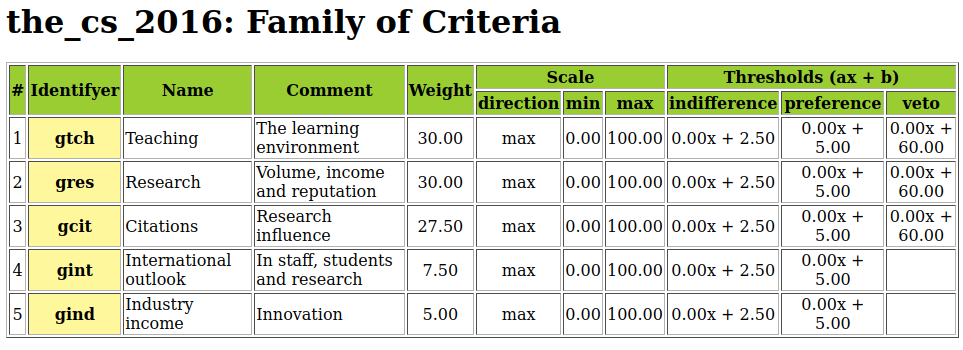
\includegraphics[width=\hsize]{Figures/13-1-the_cs_2016Criteria.png}
\caption{The THE ranking criteria}
\label{fig:13.1}       % Give a unique label
\end{figure}

Considering a very likely imprecision of the performance evaluation procedure, followed by some potential violation of uniform distributed quantile classes, we assume here that a performance quantile difference of up to $2.5\%$ is \emph{insignificant}, whereas a difference of $5\%$ and more warrants a \emph{clearly better}, resp. \emph{clearly less good} performance. With quantiles $94\%$, resp. $87.3\%$, Oxford's CS teaching environment, for instance, is thus clearly better evaluated than that of the MIT (see List.~\vref{list:13.5} Lines 27-28). We shall furthermore assume that a \emph{considerable} performance quantile difference of $60\%$, observed on the three major ranking criteria: \emph{Teaching}, \emph{Research} and \emph{Citations}, will trigger the polarisation of pairwise outranking, respectively outranked situations \citep{BIS-2013}.

The effect these performance discrimination thresholds induce on the outranking modelling can be inspected with the \texttt{showCriteria()} method\index{showCriteria@\texttt{showCriteria()}}.
\begin{lstlisting}[caption={Inspecting the performance discrimination thresholds},label=list:13.6]
>>> cspt.showCriteria()
  *----  criteria -----*
    gtch 'Teaching'
      Scale = (Decimal('0.00'), Decimal('100.00'))
      Weight = 0.300 
      Threshold ind : 2.50 + 0.00x ;   percentile:  8.07
      Threshold pref : 5.00 + 0.00x ;  percentile: 15.75
      Threshold veto : 60.00 + 0.00x ; percentile: 99.75
    gres 'Research'
      Scale = (Decimal('0.00'), Decimal('100.00'))
      Weight = 0.300 
      Threshold ind : 2.50 + 0.00x ;   percentile:  7.86
      Threshold pref : 5.00 + 0.00x ;  percentile: 16.14
      Threshold veto : 60.00 + 0.00x ; percentile: 99.21
    gcit 'Citations'
      Scale = (Decimal('0.00'), Decimal('100.00'))
      Weight = 0.275 
      Threshold ind : 2.50 + 0.00x ;   percentile:  11.82
      Threshold pref : 5.00 + 0.00x ;  percentile:  22.99
      Threshold veto : 60.00 + 0.00x ; percentile: 100.00
    gint 'International outlook'
      Scale = (Decimal('0.00'), Decimal('100.00'))
      Weight = 0.075 
      Threshold ind : 2.50 + 0.00x ;  percentile:  6.45
      Threshold pref : 5.00 + 0.00x ; percentile: 11.75
    gind 'Industry income'
      Scale = (Decimal('0.00'), Decimal('100.00'))
      Weight = 0.050 
      Threshold ind : 2.50 + 0.00x ;  percentile: 11.82
      Threshold pref : 5.00 + 0.00x ; percentile: 21.51
\end{lstlisting}

Between $6\%$ and $12\%$ of the observed quantile differences are, hence, considered to be \emph{insignificant}. Similarly, between $77\%$ and $88\%$ are considered to be \emph{significant}. Less than $1\%$ correspond to \emph{considerable} quantile differences on both the \emph{Teaching} and \emph{Research} criteria; actually triggering an epistemic polarisation effect \citep{BIS-2013}.

Beside the likely imprecise performance discrimination, the \emph{precise decimal significance weights}, as allocated by the THE authors to the five ranking criteria are, as well, quite \emph{questionable}. Criteria significance weights may carry sometimes hidden strategies for rendering the performance evaluations commensurable in view of a numerical computation of the overall ranking scores. The eventual ranking result is, the case given, as much depending on the precise values of the given criteria significance weights as, vice versa, the given precise significance weights are depending on the subjectively expected and accepted ranking results \footnote{In a social choice context, this potential double bind between voting profiles and election result, corresponds to voting manipulation strategies.}. We will therefore drop these precise decimal weights and, instead, only require a corresponding criteria significance preorder: \texttt{gtch} $=$ \texttt{gres} $>$ \texttt{gcit} $>$ \texttt{gint} $>$ \texttt{gind}. \emph{Teaching environment} and \emph{Research volume and reputation} are equally considered most significant, followed by \emph{Research influence}. Then comes \emph{International outlook in staff, students and research} and, least significant finally, \emph{Industry income and innovation}.

Both these working hypotheses: --performance discrimination thresholds and --solely ordinal criteria significance, give us way to a ranking methodology based on \emph{robust pairwise outranking} situations (see Chap.~\ref{sec:19} and \citep{BIS-2004b}).
\begin{definition}[Robust outranking situations with ordinal criteria significance weights]\label{def:13.1}
\begin{itemize}[topsep=1pt]
\item We say that CS Dept $x$ \emph{robustly outranks} CS Dept $y$ when $x$ positively outranks $y$ with \textbf{all} significance weight vectors that are compatible with the significance preorder: \texttt{gtch} $=$ \texttt{gres} $>$ \texttt{gcit} $>$ \texttt{gint} $>$ \texttt{gind};
\item We say that CS Dept $x$ is \emph{robustly outranked} by CS Dept $y$ when $x$ is positively outranked by $y$ with \textbf{all} significance weight vectors that are compatible with the significance preorder: \texttt{gtch} $=$ \texttt{gres} $>$ \texttt{gcit} $>$ \texttt{gint} $>$ \texttt{gind};
\item Otherwise, CS Depts $x$ and $y$ are considered to be \emph{incomparable}.
\end{itemize}
\end{definition}

A corresponding digraph constructor is provided by the \texttt{RobustOutranking\-Digraph} class\index{RobustOutrankingDigraph@\texttt{RobustOutrankingDigraph} class}.
\begin{lstlisting}[caption={Computing the robust outranking digraph},label=list:13.7]
>>> from outrankingDigraphs import RobustOutrankingDigraph	     
>>> rdg = RobustOutrankingDigraph(cspt)
>>> rdg
  *------- Object instance description ------*
   Instance class       : RobustOutrankingDigraph
   Instance name        : robust_the_cs_2016
   Actions              : 75
   Criteria             : 5
   Size                 : 2993
   Determinateness (%)  : 78.16
   Valuation domain     : [-1.00;1.00]
>>> rdg.computeIncomparabilityDegree(Comments=True)
  Incomparability degree (%) of digraph <robust_the_cs_2016>:
   links x<->y y: 2775, incomparable: 102, comparable: 2673
   (incomparable/links) =  0.037
>>> rdg.computeTransitivityDegree(Comments=True)
  Transitivity degree of digraph <robust_the_cs_2016>:
   triples x>y>z: 405150, closed: 218489, open: 186661
   (closed/triples) =  0.539
>>> rdg.computeSymmetryDegree(Comments=True)
  Symmetry degree (%) of digraph <robust_the_cs_2016>:
   arcs x>y: 2673, symmetric: 320, asymmetric: 2353
   (symmetric/arcs) =  0.12
\end{lstlisting}

In the resulting digraph instance \texttt{rdg} (see Line 9 in Listing~\vref{list:13.7}), we observe $2993$ such robust pairwise outranking situations validated with a mean significance of $78\%$ (Line 10). Unfortunately, in the case here, they do not deliver any complete linear ranking. The robust outranking digraph \texttt{rdg} contains 102 incomparability situations ($3.7\%$, Line 15); nearly half of its transitive closure is missing ($46.1\%$, Line 19) and $12\%$ of the positive outranking situations correspond in fact to symmetric indifference situations (Line 23).

Worse even, the digraph \texttt{rdg} admits a really high number of outranking circuits \footnote{The \texttt{computeChordlessCircuits()} and \texttt{showChordlessCircuits()} methods are separate because there are various methods available for enumerating the chordless circuits in a digraph \citep{BIS-2010}.}.\index{showChordlessCircuits@\texttt{showChordlessCircuits()}}
\begin{lstlisting}[caption={Inspecting outranking circuits},label=list:13.8]
>>> rdg.computeChordlessCircuits()
>>> rdg.showChordlessCircuits()
 *---- Chordless circuits ----*
  145 circuits.
  1:  ['albt','unlu','ariz','hels'], cred. : 0.300
  2:  ['albt','tlavu','hels'], cred. : 0.150
  3:  ['anu', 'man', 'itmo'], cred. : 0.250
  4:  ['anu', 'zhej', 'rcu'], cred. : 0.250
    ...
    ...
  82:  ['csb','epfr','rwth'], cred. : 0.250
  83:  ['csb','epfr','pud','nyu'], cred. : 0.250
  84:  ['csd','kcl','kist'], cred. : 0.250
    ...
    ...
  142:  ['kul','qut','mil'], cred. : 0.250
  143:  ['lms','rcu','tech'], cred. : 0.300
  144:  ['mil','stut','qut'], cred. : 0.300
  145:  ['mil','stut','tud'], cred. : 0.300
\end{lstlisting}

Among the 145 detected robust outranking circuits reported in Listing \vref{list:13.8}, we notice, for instance, two outranking circuits of length 4 (see circuits 1 and 83).

Let us inspect below the bipolar-valued robust outranking characteristics of the first circuit.
\begin{lstlisting}[caption={Showing the relation table with stability denotation},label=list:13.9]
>>> rdg.showRelationTable(actionsSubset=\
...         ['albt','unlu','ariz','hels'],\
...         Sorted=False) 
  * ---- Relation Table -----
   r/(stab)|  'albt' 'unlu' 'ariz' 'hels'   
      -----|-----------------------------
    'albt' |  +1.00  +0.30  +0.00  +0.00  
           |   (+4)   (+2)   (-1)   (-1)  
    'unlu' |  +0.00  +1.00  +0.40  +0.00  
           |   (+0)   (+4)   (+2)   (-1)  
    'ariz' |  +0.00  -0.12  +1.00  +0.40  
           |   (+1)   (-2)   (+4)   (+2)  
    'hels' |  +0.45  +0.00  -0.03  +1.00  
           |   (+2)   (+1)   (-2)   (+4)  
   Valuation domain: [-1.0; 1.0]
   Stability denotation semantics:
   +4|-4 : unanimous outranking | outranked situation;
   +2|-2 : outranking | outranked situation validated
      with all potential significance weights that are
      compatible with the given significance preorder;
   +1|-1 : validated outranking | outranked situation
      with the given significance weights;
     0   : indeterminate relational situation.
\end{lstlisting}

In Listing~\vref{list:13.9}, we notice that the robust outranking circuit \texttt{[albt,} \texttt{unlu,} \texttt{ariz,} \texttt{hels]}  will reappear with all potential criteria significance weight vectors that are compatible with given preorder: \texttt{gtch} $=$ \texttt{gres} $>$ \texttt{gcit} $>$ \texttt{gint} $>$ \texttt{gind}. Notice also the ($\pm 1$) marked outranking situations, like the one between \texttt{albt} and \texttt{ariz}. The statement that ``\emph{Arizona State University strictly  outranks University of Alberta}'' is in fact valid with the precise THE criteria significance weights, but not with all potential significance weights vectors that are compatible with the given significance preorder. All these ($\pm 1$)  marked outranking situations become hence \emph{doubtful} ($r(x \succsim y) = 0.00$) and the corresponding CS Depts, like University of Alberta and Arizona State University, become \emph{incomparable} in a robust outranking sense.  

Showing many incomparabilities and indifferences; not being transitive and containing many robust outranking circuits; all these relational characteristics, make that no ranking algorithm, applied to digraph \texttt{rdg}, does exist that would produce a \emph{unique} optimal linear ranking result. Methodologically, we are only left with ranking heuristics. In Chapter~\ref{sec:8} on ranking with multiple criteria we have now seen several potential heuristic ranking rules that can be used for ranking with an outranking digraph; yet, they may deliver potentially more or less diverging results. Considering the order of digraph \texttt{rdg} (75) and the largely unequal THE criteria significance weights, we rather opt, in this tutorial, for the \NetFlows ranking rule \footnote{The reader might try other ranking rules, like the \Copeland or \Kohler rules. Mind that the latter ranking-by-choosing rule is more complex (see Chap.~\ref{sec:8}).}. Its complexity in $O(n^2)$ is indeed quite tractable and, by avoiding potential \emph{tyranny of short majority} effects, the \NetFlows rule may specifically take the ranking criteria significance weights into a more fairly balanced account.

The \NetFlows ranking result of the CS Depts can be directly computed with the \texttt{computeNetFlowsRanking()} method\index{computeNetFlowsRanking@\texttt{computeNetFlowsRanking()}}. 
\begin{lstlisting}[caption={Computing a robust \NetFlows ranking},label=list:13.10]
>>> nfRanking = rdg.computeNetFlowsRanking()
>>> nfRanking
  ['ethz','calt','mit', 'oxf',  'cmel','git', 'epfl',
   'icl', 'cou', 'tum', 'wash', 'sing','hkst','ucl',
   'uiu', 'unt', 'ued', 'ntu',  'mcp', 'csd', 'cbu',
   'uta', 'tsu', 'nyu', 'uwa',  'csb', 'kit', 'utj',
   'bju', 'kcl', 'chku','kist', 'rwth','pud', 'epfr',
   'hku', 'rcu', 'cir', 'dut',  'ens', 'ntw', 'anu',
   'tub', 'mel', 'lms', 'bro',  'frei','wtu', 'tech',
   'itmo','zhej','man', 'kuj',  'kul', 'unsw','glas',
   'utw', 'unlu','naji','sou',  'hkpu','qut', 'humb',
   'shJi','stut','tud', 'tlavu','cihk','albt','indis',
   'ariz','kth', 'hels','eind', 'mil']
\end{lstlisting}

We actually obtain in Listing~\vref{list:13.10} a very similar ranking result as the one obtained with the THE average scores. The same group of seven Depts: \texttt{ethz}, \texttt{calt}, \texttt{mit}, \texttt{oxf}, \texttt{cmel}, \texttt{git} and \texttt{epfl}, is top-ranked. And a same group of Depts: \texttt{tlavu}, \texttt{cihk}, \texttt{indis}, \texttt{ariz}, \texttt{kth}, \texttt{hels}, \texttt{eind}, and \texttt{mil} appears at the end of the list.

We can print out the difference between the overall scores based THE ranking and the \NetFlows ranking above with the following short Python script, where we make use of an ordered Python dictionary with net-flow scores, stored in the \texttt{rdg.netFlowsRankingDict} attribute by the previous computation.
\begin{lstlisting}[caption={Comparing the robust \NetFlows ranking with the THE ranking},label=list:13.11,basicstyle=\ttfamily\scriptsize]
>>> # rdg.netFlowsRankingDict: ordered dictionary with net flow
>>> # scores stored in rdg by the computeNetFlowsRanking() method
>>> # theScores = [(xScore_1,x_1), (xScore_2,x_2),... ]
>>> # is sorted in decreasing order of xscores_i
>>> print(\
...  ' NetFlows ranking   gtch  gres  gcit  gint  gind   THE ranking')
>>> for i in range(75):
...     x = nfRanking[i]
...     xScore = rdg.netFlowsRankingDict[x]['netFlow']
...     thexScore,thex = theScores[i]
...     print('%2d: %s (%.2f) ' % (i+1,x,xScore), end=' \t')
...     for g in rdg.criteria:
...         print('%.1f ' % (t.evaluation[g][x]),end=' ')
...     print(' %s (%.2f)' % (thex,thexScore) )  
  NetFlows ranking   gtch  gres  gcit  gint  gind   THE ranking
   1: ethz (116.95)  89.2  97.3  97.1  93.6  64.1   ethz (92.88)
   2: calt (116.15)  91.5  96.0  99.8  59.1  85.9   calt (92.42)
   3: mit (112.72)   87.3  95.4  99.4  73.9  87.5   oxf (92.20)
   4: oxf (112.00)   94.0  92.0  98.8  93.6  44.3   mit (92.06)
   5: cmel (101.60)  88.1  92.3  99.4  58.9  71.1   git (89.88)
   6: git (93.40)    87.2  99.7  91.3  63.0  79.5   cmel (89.43)
   7: epfl (90.88)   86.3  91.6  94.8  97.2  42.7   icl (89.00)
   8: icl (90.62)    90.1  87.5  95.1  94.3  49.9   epfl (88.86)
   9: cou (84.60)    81.6  94.1  99.7  55.7  45.7   tum (87.70)
  10: tum (80.42)    87.6  95.1  87.9  52.9  95.1   sing (86.86)
  11: wash (76.28)   84.4  88.7  99.3  57.4  41.2   cou (86.59)
  12: sing (73.05)   89.9  91.3  83.0  95.3  50.6   ucl (86.05)
  13: hkst (71.05)   74.3  92.0  96.2  84.4  55.8   wash (85.60)
  14: ucl (66.78)    85.5  90.3  87.6  94.7  42.4   hkst (85.47)
  15: uiu (64.80)    85.0  83.1  99.2  51.4  42.2   ntu (85.46)
  16: unt (62.65)    79.9  84.4  99.6  77.6  38.4   ued (85.03)
  17: ued (58.67)    85.7  85.3  89.7  95.0  38.8   unt (84.42)
  18: ntu (57.88)    76.6  87.7  90.4  92.9  86.9   uiu (83.67)
  19: mcp (54.08)    79.7  89.3  94.6  29.8  51.7   mcp (81.53)
  20: csd (46.62)    75.2  81.6  99.8  39.7  59.8   cbu (81.25)
  21: cbu (44.27)    81.2  78.5  94.7  66.9  45.7   tsu (80.91)
  22: uta (43.27)    72.6  85.3  99.6  31.6  49.7   csd (80.45)
  23: tsu (42.42)    88.1  90.2  76.7  27.1  85.9   uwa (80.02)
  24: nyu (35.30)    71.1  77.4  99.4  78.0  39.8   nyu (79.72)
  25: uwa (28.88)    75.3  82.6  91.3  72.9  41.5   uta (79.61)
  26: csb (18.18)    65.6  70.9  94.8  72.9  74.9   kit (77.94)
  27: kit (16.32)    73.8  85.5  84.4  41.3  76.8   bju (77.04)
  28: utj (15.95)    92.0  91.7  48.7  25.8  49.6   csb (76.23)
  29: bju (15.45)    83.0  85.3  70.1  30.7  99.4   rwth (76.06)
  30: kcl (11.95)    45.5  94.6  86.3  95.1  38.3   hku (75.41)
  31: chku (9.43)    64.1  69.3  94.7  75.6  49.9   pud (75.17)
  32: kist (7.30)    79.4  88.2  64.2  31.6  92.8   kist (74.94)
  33: rwth (5.00)    77.8  85.0  70.8  43.7  89.4   kcl (74.81)
  34: pud (2.40)     76.9  84.8  70.8  58.1  56.7   chku (74.23)
  35: epfr (-1.70)   81.7  60.6  78.1  85.3  62.9   epfr (73.71)
  36: hku (-3.83)    77.0  73.0  77.0  96.8  39.5   dut (73.44)
  37: rcu (-6.38)    64.1  53.8  99.4  63.7  46.1   tub (73.25)
  38: cir (-8.20)    68.8  64.6  93.0  65.1  40.4   utj (72.92)
  39: dut (-8.85)    64.1  78.3  76.3  69.8  90.1   cir (72.50)
  40: ens (-8.97)    71.8  40.9  98.7  69.6  43.5   ntw (72.00)
  41: ntw (-11.15)   81.5  79.8  66.6  25.5  67.6   anu (70.57)
  42: anu (-11.50)   47.2  73.0  92.2  90.0  48.1   rcu (69.79)
  43: tub (-12.20)   66.2  82.4  71.0  55.4  99.9   mel (69.67)
  44: mel (-23.98)   56.1  70.2  83.7  83.3  50.4   lms (68.38)
  45: lms (-25.43)   81.5  68.1  61.0  31.1  87.8   ens (68.35)
  46: bro (-27.18)   58.5  54.9  96.8  52.3  38.6   wtu (67.86)
  47: frei (-34.42)  54.2  51.6  89.5  49.7  99.9   tech (67.06)
  48: wtu (-35.05)   61.8  73.5  73.7  51.9  62.2   bro (66.49)
  49: tech (-37.95)  54.9  71.0  85.1  51.7  40.1   man (66.33)
  50: itmo (-38.50)  58.0  32.0  98.7  39.2  68.7   zhej (65.34)
  51: zhej (-43.70)  73.5  70.4  60.7  22.6  75.7   frei (65.08)
  52: man (-44.83)   63.5  71.9  62.9  84.1  42.1   unsw (63.65)
  53: kuj (-47.40)   75.4  72.8  49.5  28.3  51.4   kuj (62.77)
  54: kul (-49.98)   35.2  55.8  92.0  46.0  88.3   sou (62.15)
  55: unsw (-54.88)  60.2  58.2  70.5  87.0  44.3   shJi (61.35)
  56: glas (-56.98)  35.2  52.5  91.2  85.8  39.2   itmo (60.52)
  57: utw (-59.27)   38.2  52.8  87.0  69.0  60.0   kul (60.47)
  58: unlu (-60.08)  35.2  44.2  87.4  99.7  54.1   glas (59.78)
  59: naji (-60.52)  51.4  76.9  48.8  39.7  74.4   utw (59.40)
  60: sou (-60.83)   48.2  60.7  75.5  87.4  43.2   stut (58.85)
  61: hkpu (-62.05)  46.8  36.5  91.4  73.2  41.5   naji (58.61)
  62: qut (-66.17)   45.5  42.6  82.8  75.2  63.0   tud (58.28)
  63: humb (-68.10)  48.4  31.3  94.7  41.5  45.5   unlu (58.04)
  64: shJi (-69.72)  66.9  68.3  62.4  22.8  38.5   qut (57.99)
  65: stut (-69.90)  54.2  60.6  61.1  36.3  97.8   hkpu (57.69)
  66: tud (-70.83)   46.6  53.6  75.9  53.7  66.5   albt (57.63)
  67: tlavu (-71.50) 34.1  57.2  89.0  45.3  38.6   mil (57.47)
  68: cihk (-72.20)  42.4  44.9  80.1  76.2  67.9   hels (57.40)
  69: albt (-72.33)  39.2  53.3  69.9  91.9  75.4   cihk (57.33)
  70: indis (-72.53) 56.9  76.1  49.3  20.1  41.5   tlavu (57.19)
  71: ariz (-75.10)  28.4  61.8  84.3  59.3  42.0   indis (57.04)
  72: kth (-77.10)   44.8  42.0  83.6  71.6  39.2   ariz (56.79)
  73: hels (-79.55)  48.8  49.6  80.4  50.6  39.5   kth (56.36)
  74: eind (-82.85)  32.4  48.4  81.5  72.2  45.8   humb (55.34)
  75: mil (-83.67)   46.4  64.3  69.2  44.1  38.5   eind (54.36)
\end{lstlisting}

The first inversion we observe in Listing~\vref{list:13.11} (Lines 18-19) concerns Oxford University and the MIT, switching positions 3 and 4. Most inversions are similarly short and concern only switching very close positions in either way. There are some slightly more important inversions concerning, for instance, the Hong Kong University CS Dept, ranked into position 30 in the THE ranking and here in the position 36 (Line 51). The opposite situation may also happen; the Berlin Humboldt University CS Dept, occupying the 74th position in the THE ranking, advances in the robust \NetFlows ranking to position 63 (Line 78).

In our bipolar-valued epistemic framework, the \NetFlows score of any CS Dept $x$ corresponds to the criteria significance support for the logical statement ``$x$ \emph{is first-ranked}''. Formally 
\begin{equation}\label{eq:13.1}
  r(x \; \text{is first-ranked}) \; = \; \sum_{y \neq x} r\big((x \succsim y) \,+\, (y \not\succsim x)\big) \;=\; \sum_{y \neq x} \big(r(x \succsim y) - r(y \succsim x)\big).
\end{equation}

Using the robust outranking characteristics of digraph \texttt{rdg}, we can thus explicitly compute, for instance, ETH Zürich's \NetFlows score, denoted \texttt{nfx} below.
\begin{lstlisting}
>>> x = 'ethz'
>>> nfx = Decimal('0')
>>> for y in rdg.actions:
...     if x != y:
...         nfx += (rdg.relation[x][y]\
...                - rdg.relation[y][x])  
>>> print(x, nfx)
  ethz 116.950
\end{lstlisting}

In Listing~\vref{list:13.11} (Line 16), one may now verify that ETH Zürich obtains indeed the highest \NetFlows score $116.95$, and gives, hence the \emph{most credible} first-ranked CS Dept of the 75 potential candidates.

Yet, how may we now convince the reader, that the outranking based ranking result here appears more objective and trustworthy, than the classic value theory based THE ranking by average quantile scores?  

\section{How to judge the quality of a ranking result?}
\label{sec:13.3}

In a multiple-criteria based ranking problem, inspecting pairwise marginal performance differences may give objectivity to global preferential statements. That a CS Dept $x$ convincingly outranks Dept $y$ can conveniently be checked with the \texttt{showPairwiseOutrankings()} method.\index{showPairwiseOutrankings@\texttt{showPairwiseOutrankings()}}. The ETH Zürich CS Dept is, for instance, first ranked before Caltech's Dept in both previous rankings. Lest us check the preferential reasons.
\begin{lstlisting}[caption={Comparing pairwise criteria performances},label=list:13.12,basicstyle=\ttfamily\scriptsize]
>>> rdg.showPairwiseOutrankings('ethz','calt')
  *------------  pairwise comparisons ----*
  Valuation in range: -100.00 to +100.00
  Comparing actions : ('ethz', 'calt')
  crit.    wght.  g(ethz)  g(calt) diff  | ind  pref     r()  | 
  --------------------------------------   -------------------
  'gcit'   27.50   97.10   99.80   -2.70 | 2.50  5.00   +0.00 | 
  'gind'    5.00   64.10   85.90  -21.80 | 2.50  5.00   -5.00 | 
  'gint'    7.50   93.60   59.10  +34.50 | 2.50  5.00   +7.50 | 
  'gres'   30.00   97.30   96.00   +1.30 | 2.50  5.00  +30.00 | 
  'gtch'   30.00   89.20   91.50   -2.30 | 2.50  5.00  +30.00 |
                                                     ------
                                         r(x >= y):  +62.50
  crit.    wght.  g(calt)  g(ethz) diff  | ind   pref    r()  |
  ---------------------------------------   -----------------
  'gcit'   27.50   99.80   97.10   +2.70 | 2.50  5.00  +27.50 | 
  'gind'    5.00   85.90   64.10  +21.80 | 2.50  5.00   +5.00 | 
  'gint'    7.50   59.10   93.60  -34.50 | 2.50  5.00   -7.50 | 
  'gres'   30.00   96.00   97.30   -1.30 | 2.50  5.00  +30.00 | 
  'gtch'   30.00   91.50   89.20   +2.30 | 2.50  5.00  +30.00 |
                                                      -------
                                            r(y >= x): +85.00
\end{lstlisting}

A significant positive performance difference ($+34.50$), concerning the \emph{International outlook} criterion (of $7,5\%$ significance), is observed in Listing~\vref{list:13.12} in favour of the ETH Zürich Dept (Line 9 above). Similarly, a significant positive performance difference ($+21.80$), concerning the \emph{Industry income} criterion (of $5\%$ significance), is observed, this time, in favour of the Caltech Dept (Line 17). The former, larger positive, performance difference, observed on a more significant criterion, gives so far a first convincing argument of $12.5\%$ significance for putting ETH Zürich first, before Caltech. Yet, the slightly positive performance difference ($+2.70$, Line 16) between Caltech and ETH Zürich on the \emph{Citations} criterion (of $27.5\%$ significance) confirms an ``\emph{at least as well evaluated as}'' situation in favour of the Caltech Dept.

The inverse negative performance difference ($-2.70$, Line 7), however, is neither \emph{significant} ($< -5.00$), nor \emph{insignificant} ($> -2.50$), and does hence neither confirm nor infirm a ``\emph{not at least as well evaluated as}'' situation in disfavour of ETH Zürich. We observe here a convincing argument of $27.5\%$ significance for ranking Caltech first, before ETH Zürich.

Notice finally, that, on the \emph{Teaching} and \emph{Research} criteria of total significance $60\%$, both Depts do, with performance differences $(< \mid 2.50 \mid)$, perform one as well as the other. As these two major performance criteria together necessarily admit always the highest significance with the imposed significance weight preorder: \texttt{gtch} $=$ \texttt{gres} $>$ \texttt{gcit} $>$ \texttt{gint} $>$ \texttt{gind}, both outranking situations get in fact globally confirmed at stability level $+2$ (see Chap.~\ref{sec:19}).

A browser view of the corresponding robust relation map, ordering the CS Depts again with the same \NetFlows ranking rule, well illustrates all such \emph{stable outranking} situations.
\begin{lstlisting}
>>> rdg.showHTMLRelationMap(\
...            tableTitle='Robust Outranking Map',
...            rankingRule='NetFlows')
\end{lstlisting}
\begin{figure}[ht]
%\sidecaption
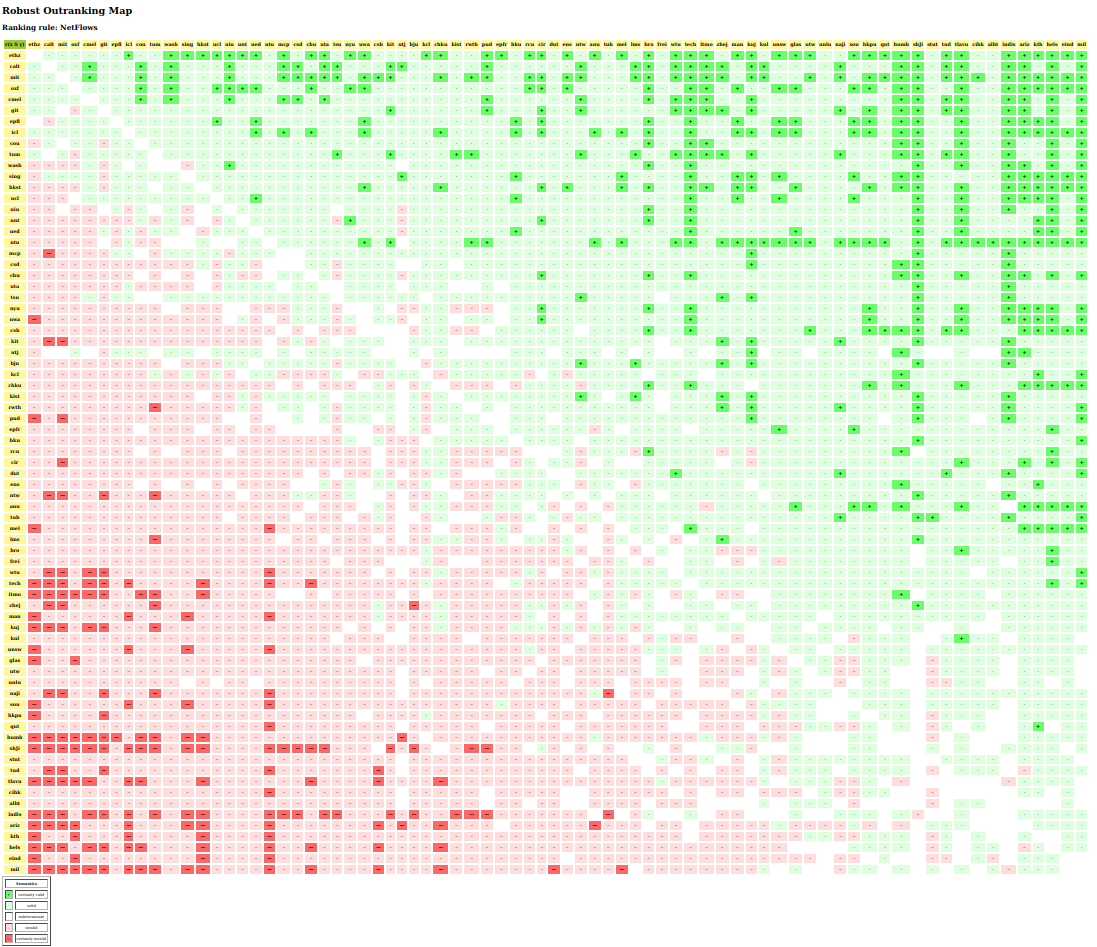
\includegraphics[width=\hsize]{Figures/13-2-the_cs_RelationMap.png}
\caption{Relation map of the robust outranking relation}
\label{fig:13.2}       % Give a unique label
\end{figure}

In Figure~\vref{fig:13.2}, \emph{dark green}, resp. \emph{light green} marked positions show certainly, resp. positively valid outranking situations, whereas \emph{dark red}, resp. \emph{light red} marked positions show certainly, respectively positively valid outranked situations. In the left upper corner one may verify that the five top-ranked Depts ([\texttt{ethz}, \texttt{calt}, \texttt{oxf}, \texttt{mit}, \texttt{cmel}]) are in fact mutually outranking each other and thus are all indifferent one to another. They give even robust \Condorcet winners by robustly outranking all other Depts.

Notice by the way that no certainly valid robust outranking (dark green) and no certainly valid robust outranked situations (dark red) appear in Figure~\vref{fig:13.3} below, resp. above the principal diagonal; none of these robust preferential situations are hence violated by the robust \NetFlows ranking. The non reflexive \emph{white} positions in the relation map, like the one between the Georgia Institute of Technology and the MIT, mark outranking or outranked situations that are not robust with respect to the given significance weight preorder. They become, hence, doubtful and are set to the indeterminate characteristic value $0.0$.

By measuring the ordinal correlation with the underlying pairwise global and marginal robust outranking situations, the quality of the robust \NetFlows ranking result can be formally evaluated with the \texttt{computeRankingCorrelation()} method\index{computeRankingCorrelation@\texttt{computeRankingCorrelation()}} and the \texttt{showCorrelation()} method\index{showCorrelation@\texttt{showCorrelation()}} (see Chap.~\ref{sec:16}).
\begin{lstlisting}[caption={Measuring the quality of the \NetFlows ranking result},label=list:13.13]
>>> corrnf = rdg.computeRankingCorrelation(nfRanking)
>>> rdg.showCorrelation(corrnf)   
  Correlation indexes:
    Crisp ordinal correlation  : +0.901
    Epistemic determination    :  0.563
    Bipolar-valued equivalence : +0.507
\end{lstlisting}

Listing~\vref{list:13.13} Line 4 indicates that the \NetFlows ranking result is indeed highly  correlated ($+0.901$, in \Kendall 's tau index sense) with the pairwise global robust outranking relation. Their bipolar-valued \emph{relational equivalence} index ($+0.51$, Line 6) indicates a more than $75\%$ criteria significance support.

With the \texttt{showRankingConsensusQuality()} method,  we can also check how the \NetFlows ranking rule is actually balancing the five ranking objectives.\index{showRankingConsensusQuality@\texttt{showRankingConsensusQua\-lity()}}
\begin{lstlisting}[caption={Measuring the consensus quality of the \NetFlows ranking result},label=list:13.14]
>>> rdg.showRankingConsensusQuality(nfRanking)
  Criterion (weight): correlation
  -------------------------------
    gtch (0.300): +0.660
    gres (0.300): +0.638
    gcit (0.275): +0.370
    gint (0.075): +0.155
    gind (0.050): +0.101
   Summary:
    Weighted mean marginal correlation (a): +0.508
    Standard deviation (b)                : +0.187
    Ranking fairness (a)-(b)              : +0.321
\end{lstlisting}

The ordinal correlation indexes with the marginal performance criterion rankings are nearly respecting the given significance weights preorder: \texttt{gtch} $\approx$ \texttt{gres} $>$ \texttt{gcit} $>$ \texttt{gint} $>$ \texttt{gind} (see Lines 4-8 above). The mean marginal ordinal correlation index is quite high ($+0.51$). Coupled with a low standard deviation ($0.187$), we obtain a quite fairly balanced ranking result (Lines 10-12). 

We can furthermore inspect with the \texttt{showCriteriaCorrelationTable()} method \index{showCriteriaCorrelationTable@\texttt{showCriteriaCorrelationTable()}} the mutual correlation indexes observed between the individual criterion based marginal robust outranking relations. 
\begin{lstlisting}[caption={Showing the ordinal correlation between the marginal criterion relations},label=list:13.15]
>>> rdg.showCriteriaCorrelationTable()
    Criteria ordinal correlation index
	 |  gcit    gind    gint    gres    gtch   
    -----|------------------------------------------
    gcit | +1.00   -0.11   +0.24   +0.13   +0.17   
    gind |         +1.00   -0.18   +0.15   +0.15   
    gint |                 +1.00   +0.04   -0.00   
    gres |                         +1.00   +0.67   
    gtch |                                 +1.00   
\end{lstlisting}

Slightly contradictory ($-0.11$) appear the \emph{Citations} and \emph{Industrial income} criteria (Line 5 Column 3 in List.~\vref{list:13.15}). Due perhaps to potential confidentiality clauses, it seams perhaps not always possible to publish industrially relevant research results in highly ranked journals. However, criteria \emph{Citations} and \emph{International outlook} show a slightly positive correlation ($+0.24$, Column 4), whereas the \emph{International outlook} criterion shows no apparent correlation with both the major \emph{Teaching} and \emph{Research} criteria. The latter are however highly correlated ($+0.67$. Line 9 Column 6).

A Principal Component Analysis may well illustrate with the \texttt{export3Dplot\-OfCriteriaCorrelation()} method the previous findings \citep{CPSTAT-L2}. \index{export3DplotOfCriteriaCorrelation@\texttt{export3DplotOfCriteria\-Correlation()}}
\begin{lstlisting}
>>> rdg.export3DplotOfCriteriaCorrelation(graphType='pdf')
\end{lstlisting}
\begin{figure}[ht]
%\sidecaption
\includegraphics[width=\hsize]{Figures/13-3-3DCorrelation.pdf}
\caption{3D PCA plot of the pairwise criteria correlation table}
\label{fig:13.3}       % Give a unique label
\end{figure}

In Figure~\vref{fig:13.3}, one may notice first that more than $80\%$ of the total variance of the previous correlation table is explained by the apparent opposition between the marginal outrankings of criteria: \emph{Teaching}, \emph{Research} and \emph{Industry income} on the left side, and the marginal outrankings of criteria: \emph{Citations} and \emph{International outlook} on the right side. Notice also in the left lower corner the nearly identical positions of the marginal outrankings of the major \emph{Teaching} and \emph{Research} criteria. In the factors 2 and 3 plot, about $30\%$ of the total variance is captured by the opposition between the marginal outrankings of the \emph{Teaching} and \emph{Research} criteria and the marginal outrankings of the \emph{Industrial income} criterion. Finally, in the factors 1 and 3 plot, nearly $15\%$ of the total variance is explained by the opposition between the marginal outrankings of the \emph{International outlook} criterion and the marginal outrankings of the \emph{Citations} criterion.

It is, finally, interesting to similarly assess the ordinal correlation between the THE average scores-based ranking and the robust outranking digraph.
\begin{lstlisting}[caption={Computing the ordinal quality of the THE ranking},label=list:13.16]
>>> # theScores = [(xScore_1,x_1), (xScore_2,x_2),... ]
>>> # is sorted in decreasing order of xscores
>>> theRanking = [item[1] for item in theScores]
>>> corrthe = rdg.computeRankingCorrelation(theRanking)
>>> rdg.showCorrelation(corrthe)
    Correlation indexes:
     Crisp ordinal correlation  : +0.907
     Epistemic determination    :  0.563
     Bipolar-valued equivalence : +0.511
>>> rdg.showRankingConsensusQuality(theRanking)
    Criterion (weight): correlation
    -------------------------------
     gtch (0.300): +0.683
     gres (0.300): +0.670
     gcit (0.275): +0.319
     gint (0.075): +0.161
     gind (0.050): +0.106
    Summary:
     Weighted mean marginal correlation (a): +0.511
     Standard deviation (b)                : +0.210
     Ranking fairness (a)-(b)              : +0.302
\end{lstlisting}

The THE ranking result is similarly correlated ($+0.907$, Line 7 in List.~\ref{list:13.16}) with the pairwise global robust outranking situations. By its overall weighted scoring rule, the THE ranking naturally induces marginal criterion correlations that are compatible with the given significance weight preorder (Lines 13-17). Notice that the mean marginal correlation is of a similar value ($+0.51$, Line 19) as the robust \NetFlows ranking. Yet, its standard deviation is slightly higher, which leads to a less fairer balancing of the three major ranking criteria.

To conclude, let us emphasise, that, without any commensurability hypothesis and by taking, furthermore, into account, first, the always present more or less imprecision of any performance evaluation and, secondly, solely ordinal criteria significance weights, we may obtain here with our robust outranking approach a very similar ranking result with a slightly better preference modelling quality. A convincing heatmap view of the 25 first-ranked Institutions may eventually be generated in the default system browser with following command.
\begin{lstlisting}
>>> rdg.showHTMLPerformanceHeatmap(
...            WithActionNames=True,\
...            outrankingModel='this',\
...            rankingRule='NetFlows',\
...            ndigits=1,\
...            Correlations=True,\
...            fromIndex=0,toIndex=25)
\end{lstlisting}
\begin{figure}[ht]
%\sidecaption
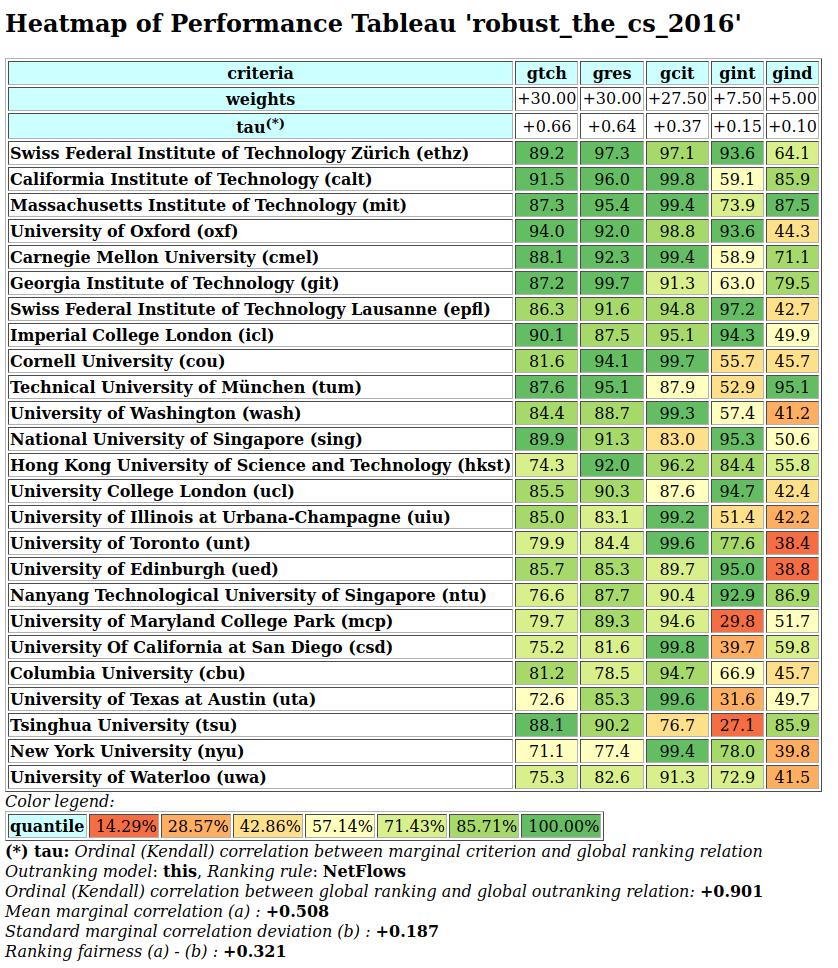
\includegraphics[width=\hsize]{Figures/13-4-theHeatmap.png}
\caption{Extract of a heatmap browser view on the \NetFlows ranking result}
\label{fig:13.4}       % Give a unique label
\end{figure}

As an exercise, the reader is invited to try out other robust outranking based ranking heuristics. Notice also that we have not challenged in this case study the THE provided criteria significance preorder. It would be very interesting to consider the five ranking objectives as equally important and, consequently, consider the ranking criteria to be equisignificant. Curious to see the ranking results under such settings.
 
%%%%%%% The chapter bibliography
%\normallatexbib
%\clearpage
\phantomsection
\addcontentsline{toc}{section}{Chapter Bibliography}
\chapter{The best academic Computer Science Depts: A ranking case study}
\label{sec:13}

\abstract*{ In this case study, we are solving with our \Digraph resources a ranking decision problem based on published data from the \emph{Times Higher Education} (THE) \emph{World University Rankings} 2016 by \emph{Computer Science} (CS) subject. Several hundred academic CS Departments, from all over the world, were ranked that year following an overall numerical score based on the weighted average of five performance criteria: \emph{Teaching} (the learning environment, $30\%$), \emph{Research} (volume, income and reputation, $30\%$), \emph{Citations} (research influence, $27.5\%$), \emph{International outlook} (staff, students, and research, $7.5\%$), and \emph{Industry income} (innovation, $5\%$). To illustrate our \Digraph programming resources, we shall first have a look into the THE ranking data with short Python scripts. In a second section, we shall relax the commensurability hypothesis of the ranking criteria and show how to similarly rank with multiple incommensurable performance criteria of solely ordinal significance. A third Section is finally devoted to introduce quality measures for qualifying ranking results.}

\abstract{ In this case study, we are solving with our \Digraph resources a ranking decision problem based on published data from the \emph{Times Higher Education} (THE) \emph{World University Rankings} 2016 by \emph{Computer Science} (CS) subject. Several hundred academic CS Departments, from all over the world, were ranked that year following an overall numerical score based on the weighted average of five performance criteria: \emph{Teaching} (the learning environment, $30\%$), \emph{Research} (volume, income and reputation, $30\%$), \emph{Citations} (research influence, $27.5\%$), \emph{International outlook} (staff, students, and research, $7.5\%$), and \emph{Industry income} (innovation, $5\%$). To illustrate our \Digraph programming resources, we shall first have a look into the THE multiple-criteria ranking data with short Python scripts. In a second section, we shall relax the commensurability hypothesis of the ranking criteria and show how to similarly rank with multiple incommensurable performance criteria of solely ordinal significance. A third section is finally devoted to introduce quality measures for qualifying ranking results.
}

\section{The THE performance tableau}
\label{sec:13.1}

For this decision making case study, we use an extract of the published \THE (THE) World University rankings 2016 by Computer Science (CS) subject, concerning the 75 first-ranked academic Institutions\footnote{\href{https://www.timeshighereducation.com/world-university-rankings/2017/subject-ranking/computer-science}{THE World University Rankings 2016 by Computer Science subject}}. The multiple-criteria performance tableau data, collected from the THE web pages, is stored in a file named \texttt{the-cs-2016.py} of \texttt{PerformanceTableau} format \footnote{The performance tableau \texttt{the-cs-2016.py} is available in the \texttt{examples} directory of the \Digraph resources \citep{BIS-2021}.}.\index{THE University rankings 2016 by CS subject} 
\begin{lstlisting}[caption={Performance tableau of the },label=list:13.1]
>>> from perfTabs import PerformanceTableau
>>> cspt = PerformanceTableau('the_cs_2016')
>>> cspt
  *------- PerformanceTableau instance description ------*
   Instance class     : PerformanceTableau
   Instance name      : the-cs-2016
   Actions            : 75
   Objectives         : 5
   Criteria           : 5
   NaN proportion (%) : 0.0
   Attributes         : ['name','description','actions',
                           'objectives','criteria',
			   'weightPreorder','NA','evaluation']
\end{lstlisting}

Potential decision alternatives, in our case here, are the 75 THE best-ranked CS Departments in 2016, all of them located at world renowned Institutions, like California Institute of Technology, Swiss Federal Institute of Technology Zurich, Technical University München, University of Oxford or the National University of Singapore (see List.~\vref{list:13.2} below). 

Instead of using prefigured \Digraph \texttt{show...()} methods, readily available for inspecting \texttt{PerformanceTableau} instances, Listing~\vref{list:13.2} illustrates how to write small Python scripts for printing out its content.   
\begin{lstlisting}[caption={Printing the CS Departments},label=list:13.2,basicstyle=\ttfamily\scriptsize]
>>> for x in cspt.actions:
...     print('%s:\t%s (%s)' %\
...        (x,cspt.actions[x]['name'],cspt.actions[x]['comment']) )
  albt:	University of Alberta (CA)
  anu:	Australian National University (AU)
  ariz:	Arizona State University (US)
  bju:	Beijing University (CN)
  bro:	Brown University (US)
  calt:	California Institute of Technology (US)
  cbu:	Columbia University (US)
  chku:	Chinese University of Hong Kong (HK)
  cihk:	City University of Hong Kong (HK)
  cir:	University of California at Irvine (US)
  cmel:	Carnegie Mellon University (US)
  cou:	Cornell University (US)
  csb:	University of California at Santa Barbara (US)
  csd:	University Of California at San Diego (US)
  dut:	Delft University of Technology (NL)
  eind:	Eindhoven University of Technology (NL)
  ens:	Superior Normal School at Paris (FR)
  epfl:	Swiss Federal Institute of Technology Lausanne (CH)
  epfr:	Polytechnic school of Paris (FR)
  ethz:	Swiss Federal Institute of Technology Zurich (CH)
  frei:	University of Freiburg (DE)
  git:	Georgia Institute of Technology (US)
  glas:	University of Glasgow (UK)
  hels:	University of Helsinki (FI)
  hkpu:	Hong Kong Polytechnic University (CN)
  hkst:	Hong Kong University of Science and Technology (HK)
  hku:	Hong Kong University (HK)
  humb:	Berlin Humboldt University (DE)
  icl:	Imperial College London (UK)
  indis:Indian Institute of Science (IN)
  itmo:	ITMO University (RU)
  kcl:	King's College London (UK)
  kist:	Korea Adv. Institute of Science and Technology (KR)
  kit:	Karlsruhe Institute of Technology (DE)
  kth:	KTH Royal Institute of Technology (SE)
  kuj:	Kyoto University (JP)
  kul:	Catholic University Leuven (BE)
  lms:	Lomonosov Moscow State University (RU)
  man:	University of Manchester (UK)
  mcp:	University of Maryland College Park (US)
  mel:	University of Melbourne (AU)
  mil:	Polytechnic University of Milan (IT)
  mit:	Massachusetts Institute of Technology (US)
  naji:	Nanjing University (CN)
  ntu:	Nanyang Technological University of Singapore (SG)
  ntw:	National Taiwan University (TW)
  nyu:	New York University (US)
  oxf:	University of Oxford (UK)
  pud:	Purdue University (US)
  qut:	Queensland University of Technology (AU)
  rcu:	Rice University (US)
  rwth:	RWTH Aachen University (DE)
  shJi:	Shanghai Jiao Tong University (CN)
  sing:	National University of Singapore (SG)
  sou:	University of Southhampton (UK)
  stut:	University of Stuttgart (DE)
  tech:	Technion - Israel Institute of Technology (IL)
  tlavu:Tel Aviv University (IR)
  tsu:	Tsinghua University (CN)
  tub:	Technical University of Berlin (DE)
  tud:	Technical University of Darmstadt (DE)
  tum:	Technical University of Muenchen (DE)
  ucl:	University College London (UK)
  ued:	University of Edinburgh (UK)
  uiu:	University of Illinois at Urbana-Champagne (US)
  unlu:	University of Luxembourg (LU)
  unsw:	University of New South Wales (AU)
  unt:	University of Toronto (CA)
  uta:	University of Texas at Austin (US)
  utj:	University of Tokyo (JP)
  utw:	University of Twente (NL)
  uwa:	University of Waterloo (CA)
  wash:	University of Washington (US)
  wtu:	Vienna University of Technology (AUS)
  zhej:	Zhejiang University (CN)
\end{lstlisting}

The THE authors base their 2016 ranking on five decision objectives \citep{THE-2016}.
\begin{lstlisting}[caption={The THE ranking objectives},label=list:13.3,basicstyle=\ttfamily\scriptsize]
>>> for obj in cspt.objectives:
...     print('%s: %s (%.1f%%),\n\t%s' %\
...                (obj,cspt.objectives[obj]['name'],\
...                 cspt.objectives[obj]['weight'],
...                 cspt.objectives[obj]['comment'])\
...           ) 
 Teaching: Best learning environment (30.0%)
   Reputation survey; Staff-to-student ration;
   Doctorate-to-student ratio;
   Doctorate-to-academic-staff ratio;
   Institutional income.
 Research: Highest volume and reputation (30.0%)
   Reputation survey;
   Research income;
   Research productivity.
 Citations: Highest research influence (27.5%)
   Impact.
 International outlook: Most international staff,
                        students and research (7.5%)
   Proportions of international students;
   Proportions of international staff;
   International collaborations.
 Industry income: Best knowledge transfer (5.0%)
   Volume.
\end{lstlisting}

With a cumulated importance of $87\%$ (see above), \emph{Teaching}, \emph{Research} and \emph{Citations} represent clearly the major ranking objectives. \emph{International outlook} and \emph{Industry income} are considered of minor importance ($12.5\%$).

THE authors do, unfortunately, not publish the detail of their performance assessments for evaluating CS Depts with respect to each one of performance criteria per ranking objective.  \footnote{THE gives some insight on the subject and significance of the actual ranking criteria used for evaluating along each ranking objective on her website \citep{THE-2016}}. The THE 2016 ranking publication reveals solely a compound assessment on a single performance criteria per ranking objective. The five retained performance criteria may be printed out as follows.
\begin{lstlisting}
>>> for g in cspt.criteria:
...     print('%s:\t%s, %s (%.1f%%)' %\
...       (g,cspt.criteria[g]['name'],cspt.criteria[g]['comment'],\
...        cspt.criteria[g]['weight']) )  
  gtch:	Teaching, The learning environment (30.0%)
  gres:	Research, Volume, income and reputation (30.0%)
  gcit:	Citations, Research influence (27.5%)
  gint:	International outlook, In staff, students and research (7.5%)
  gind:	Industry income, knowledge transfer (5.0%)
\end{lstlisting}

The largest part ($87.5\%$) of criteria significance is, hence canonically, allocated to the major ranking criteria: \emph{Teaching} ($30\%$), \emph{Research} ($30\%$) and \emph{Citations} ($27.5\%$). The small remaining part ($12.5\%$) goes to \emph{International outlook} ($7.5\%$) and \emph{Industry income} ($5\%$).

In order to render commensurable these performance criteria, the THE authors replace, per criterion, the actual performance evaluation obtained by each University with the corresponding \emph{quantile} observed in the cumulative distribution of the performance evaluations obtained by all the surveyed institutions \citep{THE-2016}. The THE ranking is eventually determined by an \emph{overall score} per University which corresponds to the weighted average of these five criteria quantiles, as illustrated in Listing~\vref{list:13.4}.     
\begin{lstlisting}[caption={Computing the THE overall scores},label=list:13.4]
>>> theScores = []
>>> for x in cspt.actions:
...     xscore = Decimal('0')
...     for g in cspt.criteria:
...         xscore += cspt.evaluation[g][x] *\
...          (cspt.criteria[g]['weight']/Decimal('100'))
...	   theScores.append((xscore,x))
\end{lstlisting}

In Listing~\vref{list:13.5} (Lines 15-16), we may thus notice that, in the 2016 edition of the THE World University rankings by CS subject, the Swiss Federal Institute of Technology Zürich is first-ranked with an overall score of $92.9$; followed by the California Institute of Technology (overall score: $92.4$) \footnote{The author's own Computer Science Dept at the University of Luxembourg was ranked on position 63 with an overall score of $58.0$.}.
\begin{lstlisting}[caption={Printing the ranked performance table},label=list:13.5,basicstyle=\ttfamily\scriptsize]
>>> theScores.sort(reverse = True)
>>> print('##  Univ \tgtch  gres  gcit  gint  gind  overall')
>>> print('-------------------------------------------------') 
>>> i = 1
>>> for it in theScores:
...     x = it[1]
...     xScore = it[0]
...     print('%2d: %s' % (i,x), end=' \t')
...     for g in cspt.criteria:
...         print('%.1f ' % (cspt.evaluation[g][x]),end=' ')
...	    print(' %.1f' % xScore)
...         i += 1   
    ##  Univ 	gtch  gres  gcit  gint  gind  overall
    -------------------------------------------------
     1: ethz 	89.2  97.3  97.1  93.6  64.1   92.9
     2: calt 	91.5  96.0  99.8  59.1  85.9   92.4
     3: oxf 	94.0  92.0  98.8  93.6  44.3   92.2
     4: mit 	87.3  95.4  99.4  73.9  87.5   92.1
     5: git 	87.2  99.7  91.3  63.0  79.5   89.9
     6: cmel 	88.1  92.3  99.4  58.9  71.1   89.4
     7: icl 	90.1  87.5  95.1  94.3  49.9   89.0
     8: epfl 	86.3  91.6  94.8  97.2  42.7   88.9
     9: tum 	87.6  95.1  87.9  52.9  95.1   87.7
    10: sing 	89.9  91.3  83.0  95.3  50.6   86.9
    11: cou 	81.6  94.1  99.7  55.7  45.7   86.6
    12: ucl 	85.5  90.3  87.6  94.7  42.4   86.1
    13: wash 	84.4  88.7  99.3  57.4  41.2   85.6
    14: hkst 	74.3  92.0  96.2  84.4  55.8   85.5
    15: ntu 	76.6  87.7  90.4  92.9  86.9   85.5
    16: ued 	85.7  85.3  89.7  95.0  38.8   85.0
    17: unt 	79.9  84.4  99.6  77.6  38.4   84.4
    18: uiu 	85.0  83.1  99.2  51.4  42.2   83.7
    19: mcp 	79.7  89.3  94.6  29.8  51.7   81.5
    20: cbu 	81.2  78.5  94.7  66.9  45.7   81.3
    21: tsu 	88.1  90.2  76.7  27.1  85.9   80.9
    22: csd 	75.2  81.6  99.8  39.7  59.8   80.5
    23: uwa 	75.3  82.6  91.3  72.9  41.5   80.0
    24: nyu 	71.1  77.4  99.4  78.0  39.8   79.7
    25: uta 	72.6  85.3  99.6  31.6  49.7   79.6
    26: kit 	73.8  85.5  84.4  41.3  76.8   77.9
    27: bju 	83.0  85.3  70.1  30.7  99.4   77.0
    28: csb 	65.6  70.9  94.8  72.9  74.9   76.2
    29: rwth 	77.8  85.0  70.8  43.7  89.4   76.1
    30: hku 	77.0  73.0  77.0  96.8  39.5   75.4
    31: pud 	76.9  84.8  70.8  58.1  56.7   75.2
    32: kist 	79.4  88.2  64.2  31.6  92.8   74.9
    33: kcl 	45.5  94.6  86.3  95.1  38.3   74.8
    34: chku 	64.1  69.3  94.7  75.6  49.9   74.2
    35: epfr 	81.7  60.6  78.1  85.3  62.9   73.7
    36: dut 	64.1  78.3  76.3  69.8  90.1   73.4
    37: tub 	66.2  82.4  71.0  55.4  99.9   73.3
    38: utj 	92.0  91.7  48.7  25.8  49.6   72.9
    39: cir 	68.8  64.6  93.0  65.1  40.4   72.5
    40: ntw 	81.5  79.8  66.6  25.5  67.6   72.0
    41: anu 	47.2  73.0  92.2  90.0  48.1   70.6
    42: rcu 	64.1  53.8  99.4  63.7  46.1   69.8
    43: mel 	56.1  70.2  83.7  83.3  50.4   69.7
    44: lms 	81.5  68.1  61.0  31.1  87.8   68.4
    45: ens 	71.8  40.9  98.7  69.6  43.5   68.3
    46: wtu 	61.8  73.5  73.7  51.9  62.2   67.9
    47: tech 	54.9  71.0  85.1  51.7  40.1   67.1
    48: bro 	58.5  54.9  96.8  52.3  38.6   66.5
    49: man 	63.5  71.9  62.9  84.1  42.1   66.3
    50: zhej 	73.5  70.4  60.7  22.6  75.7   65.3
    51: frei 	54.2  51.6  89.5  49.7  99.9   65.1
    52: unsw 	60.2  58.2  70.5  87.0  44.3   63.6
    53: kuj 	75.4  72.8  49.5  28.3  51.4   62.8
    54: sou 	48.2  60.7  75.5  87.4  43.2   62.1
    55: shJi 	66.9  68.3  62.4  22.8  38.5   61.4
    56: itmo 	58.0  32.0  98.7  39.2  68.7   60.5
    57: kul 	35.2  55.8  92.0  46.0  88.3   60.5
    58: glas 	35.2  52.5  91.2  85.8  39.2   59.8
    59: utw 	38.2  52.8  87.0  69.0  60.0   59.4
    60: stut 	54.2  60.6  61.1  36.3  97.8   58.9
    61: naji 	51.4  76.9  48.8  39.7  74.4   58.6
    62: tud 	46.6  53.6  75.9  53.7  66.5   58.3
    63: unlu 	35.2  44.2  87.4  99.7  54.1   58.0
    64: qut 	45.5  42.6  82.8  75.2  63.0   58.0
    65: hkpu 	46.8  36.5  91.4  73.2  41.5   57.7
    66: albt 	39.2  53.3  69.9  91.9  75.4   57.6
    67: mil 	46.4  64.3  69.2  44.1  38.5   57.5
    68: hels 	48.8  49.6  80.4  50.6  39.5   57.4
    69: cihk 	42.4  44.9  80.1  76.2  67.9   57.3
    70: tlavu 	34.1  57.2  89.0  45.3  38.6   57.2
    71: indis 	56.9  76.1  49.3  20.1  41.5   57.0
    72: ariz 	28.4  61.8  84.3  59.3  42.0   56.8
    73: kth 	44.8  42.0  83.6  71.6  39.2   56.4
    74: humb 	48.4  31.3  94.7  41.5  45.5   55.3
    75: eind 	32.4  48.4  81.5  72.2  45.8   54.4
\end{lstlisting}

It is important to notice that a ranking by weighted average scores requires \emph{commensurable ranking criteria} of precise decimal significance and on wich precise decimal performance evaluations are given. It is very unlikely that the THE 2016 performance assessments verify indeed these conditions. Here we show how to relax these methodological requirements --precise commensurable criteria and decimal evaluations-- by following instead a bipolar-valued epistemic logic based ranking methodology (see Chap.~\ref{sec:8}).

\section{Ranking with multiple criteria of ordinal significance}
\label{sec:13.2}

Let us, first, have a critical look in Figure~\vref{fig:13.1} at the THE performance criteria.
\begin{lstlisting}
>>> cspt.showHTMLCriteria(Sorted=False)
\end{lstlisting}
\begin{figure}[ht]
%\sidecaption
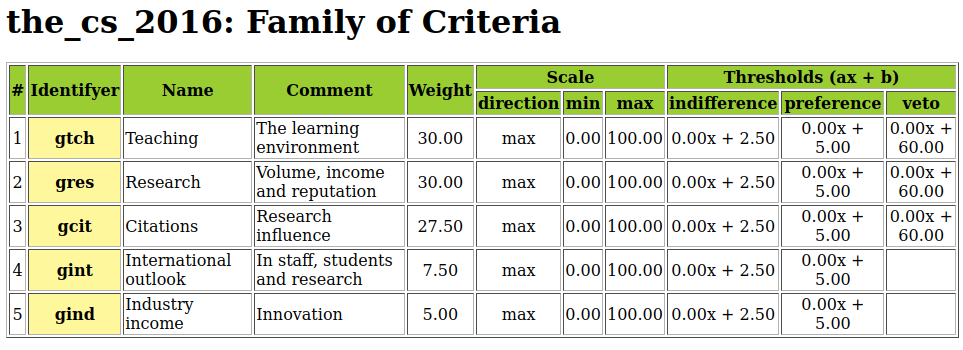
\includegraphics[width=\hsize]{Figures/13-1-the_cs_2016Criteria.png}
\caption{The THE ranking criteria}
\label{fig:13.1}       % Give a unique label
\end{figure}

Considering a very likely imprecision of the performance evaluation procedure, followed by some potential violation of uniform distributed quantile classes, we assume here that a performance quantile difference of up to $2.5\%$ is \emph{insignificant}, whereas a difference of $5\%$ and more warrants a \emph{clearly better}, resp. \emph{clearly less good} performance. With quantiles $94\%$, resp. $87.3\%$, Oxford's CS teaching environment, for instance, is thus clearly better evaluated than that of the MIT (see List.~\vref{list:13.5} Lines 27-28). We shall furthermore assume that a \emph{considerable} performance quantile difference of $60\%$, observed on the three major ranking criteria: \emph{Teaching}, \emph{Research} and \emph{Citations}, will trigger the polarisation of pairwise outranking, respectively outranked situations \citep{BIS-2013}.

The effect these performance discrimination thresholds induce on the outranking modelling can be inspected with the \texttt{showCriteria()} method\index{showCriteria@\texttt{showCriteria()}}.
\begin{lstlisting}[caption={Inspecting the performance discrimination thresholds},label=list:13.6]
>>> cspt.showCriteria()
  *----  criteria -----*
    gtch 'Teaching'
      Scale = (Decimal('0.00'), Decimal('100.00'))
      Weight = 0.300 
      Threshold ind : 2.50 + 0.00x ;   percentile:  8.07
      Threshold pref : 5.00 + 0.00x ;  percentile: 15.75
      Threshold veto : 60.00 + 0.00x ; percentile: 99.75
    gres 'Research'
      Scale = (Decimal('0.00'), Decimal('100.00'))
      Weight = 0.300 
      Threshold ind : 2.50 + 0.00x ;   percentile:  7.86
      Threshold pref : 5.00 + 0.00x ;  percentile: 16.14
      Threshold veto : 60.00 + 0.00x ; percentile: 99.21
    gcit 'Citations'
      Scale = (Decimal('0.00'), Decimal('100.00'))
      Weight = 0.275 
      Threshold ind : 2.50 + 0.00x ;   percentile:  11.82
      Threshold pref : 5.00 + 0.00x ;  percentile:  22.99
      Threshold veto : 60.00 + 0.00x ; percentile: 100.00
    gint 'International outlook'
      Scale = (Decimal('0.00'), Decimal('100.00'))
      Weight = 0.075 
      Threshold ind : 2.50 + 0.00x ;  percentile:  6.45
      Threshold pref : 5.00 + 0.00x ; percentile: 11.75
    gind 'Industry income'
      Scale = (Decimal('0.00'), Decimal('100.00'))
      Weight = 0.050 
      Threshold ind : 2.50 + 0.00x ;  percentile: 11.82
      Threshold pref : 5.00 + 0.00x ; percentile: 21.51
\end{lstlisting}

Between $6\%$ and $12\%$ of the observed quantile differences are, hence, considered to be \emph{insignificant}. Similarly, between $77\%$ and $88\%$ are considered to be \emph{significant}. Less than $1\%$ correspond to \emph{considerable} quantile differences on both the \emph{Teaching} and \emph{Research} criteria; actually triggering an epistemic polarisation effect \citep{BIS-2013}.

Beside the likely imprecise performance discrimination, the \emph{precise decimal significance weights}, as allocated by the THE authors to the five ranking criteria are, as well, quite \emph{questionable}. Criteria significance weights may carry sometimes hidden strategies for rendering the performance evaluations commensurable in view of a numerical computation of the overall ranking scores. The eventual ranking result is, the case given, as much depending on the precise values of the given criteria significance weights as, vice versa, the given precise significance weights are depending on the subjectively expected and accepted ranking results \footnote{In a social choice context, this potential double bind between voting profiles and election result, corresponds to voting manipulation strategies.}. We will therefore drop these precise decimal weights and, instead, only require a corresponding criteria significance preorder: \texttt{gtch} $=$ \texttt{gres} $>$ \texttt{gcit} $>$ \texttt{gint} $>$ \texttt{gind}. \emph{Teaching environment} and \emph{Research volume and reputation} are equally considered most significant, followed by \emph{Research influence}. Then comes \emph{International outlook in staff, students and research} and, least significant finally, \emph{Industry income and innovation}.

Both these working hypotheses: --performance discrimination thresholds and --solely ordinal criteria significance, give us way to a ranking methodology based on \emph{robust pairwise outranking} situations (see Chap.~\ref{sec:19} and \citep{BIS-2004b}).
\begin{definition}[Robust outranking situations with ordinal criteria significance weights]\label{def:13.1}
\begin{itemize}[topsep=1pt]
\item We say that CS Dept $x$ \emph{robustly outranks} CS Dept $y$ when $x$ positively outranks $y$ with \textbf{all} significance weight vectors that are compatible with the significance preorder: \texttt{gtch} $=$ \texttt{gres} $>$ \texttt{gcit} $>$ \texttt{gint} $>$ \texttt{gind};
\item We say that CS Dept $x$ is \emph{robustly outranked} by CS Dept $y$ when $x$ is positively outranked by $y$ with \textbf{all} significance weight vectors that are compatible with the significance preorder: \texttt{gtch} $=$ \texttt{gres} $>$ \texttt{gcit} $>$ \texttt{gint} $>$ \texttt{gind};
\item Otherwise, CS Depts $x$ and $y$ are considered to be \emph{incomparable}.
\end{itemize}
\end{definition}

A corresponding digraph constructor is provided by the \texttt{RobustOutranking\-Digraph} class\index{RobustOutrankingDigraph@\texttt{RobustOutrankingDigraph} class}.
\begin{lstlisting}[caption={Computing the robust outranking digraph},label=list:13.7]
>>> from outrankingDigraphs import RobustOutrankingDigraph	     
>>> rdg = RobustOutrankingDigraph(cspt)
>>> rdg
  *------- Object instance description ------*
   Instance class       : RobustOutrankingDigraph
   Instance name        : robust_the_cs_2016
   Actions              : 75
   Criteria             : 5
   Size                 : 2993
   Determinateness (%)  : 78.16
   Valuation domain     : [-1.00;1.00]
>>> rdg.computeIncomparabilityDegree(Comments=True)
  Incomparability degree (%) of digraph <robust_the_cs_2016>:
   links x<->y y: 2775, incomparable: 102, comparable: 2673
   (incomparable/links) =  0.037
>>> rdg.computeTransitivityDegree(Comments=True)
  Transitivity degree of digraph <robust_the_cs_2016>:
   triples x>y>z: 405150, closed: 218489, open: 186661
   (closed/triples) =  0.539
>>> rdg.computeSymmetryDegree(Comments=True)
  Symmetry degree (%) of digraph <robust_the_cs_2016>:
   arcs x>y: 2673, symmetric: 320, asymmetric: 2353
   (symmetric/arcs) =  0.12
\end{lstlisting}

In the resulting digraph instance \texttt{rdg} (see Line 9 in Listing~\vref{list:13.7}), we observe $2993$ such robust pairwise outranking situations validated with a mean significance of $78\%$ (Line 10). Unfortunately, in the case here, they do not deliver any complete linear ranking. The robust outranking digraph \texttt{rdg} contains 102 incomparability situations ($3.7\%$, Line 15); nearly half of its transitive closure is missing ($46.1\%$, Line 19) and $12\%$ of the positive outranking situations correspond in fact to symmetric indifference situations (Line 23).

Worse even, the digraph \texttt{rdg} admits a really high number of outranking circuits \footnote{The \texttt{computeChordlessCircuits()} and \texttt{showChordlessCircuits()} methods are separate because there are various methods available for enumerating the chordless circuits in a digraph \citep{BIS-2010}.}.\index{showChordlessCircuits@\texttt{showChordlessCircuits()}}
\begin{lstlisting}[caption={Inspecting outranking circuits},label=list:13.8]
>>> rdg.computeChordlessCircuits()
>>> rdg.showChordlessCircuits()
 *---- Chordless circuits ----*
  145 circuits.
  1:  ['albt','unlu','ariz','hels'], cred. : 0.300
  2:  ['albt','tlavu','hels'], cred. : 0.150
  3:  ['anu', 'man', 'itmo'], cred. : 0.250
  4:  ['anu', 'zhej', 'rcu'], cred. : 0.250
    ...
    ...
  82:  ['csb','epfr','rwth'], cred. : 0.250
  83:  ['csb','epfr','pud','nyu'], cred. : 0.250
  84:  ['csd','kcl','kist'], cred. : 0.250
    ...
    ...
  142:  ['kul','qut','mil'], cred. : 0.250
  143:  ['lms','rcu','tech'], cred. : 0.300
  144:  ['mil','stut','qut'], cred. : 0.300
  145:  ['mil','stut','tud'], cred. : 0.300
\end{lstlisting}

Among the 145 detected robust outranking circuits reported in Listing \vref{list:13.8}, we notice, for instance, two outranking circuits of length 4 (see circuits 1 and 83).

Let us inspect below the bipolar-valued robust outranking characteristics of the first circuit.
\begin{lstlisting}[caption={Showing the relation table with stability denotation},label=list:13.9]
>>> rdg.showRelationTable(actionsSubset=\
...         ['albt','unlu','ariz','hels'],\
...         Sorted=False) 
  * ---- Relation Table -----
   r/(stab)|  'albt' 'unlu' 'ariz' 'hels'   
      -----|-----------------------------
    'albt' |  +1.00  +0.30  +0.00  +0.00  
           |   (+4)   (+2)   (-1)   (-1)  
    'unlu' |  +0.00  +1.00  +0.40  +0.00  
           |   (+0)   (+4)   (+2)   (-1)  
    'ariz' |  +0.00  -0.12  +1.00  +0.40  
           |   (+1)   (-2)   (+4)   (+2)  
    'hels' |  +0.45  +0.00  -0.03  +1.00  
           |   (+2)   (+1)   (-2)   (+4)  
   Valuation domain: [-1.0; 1.0]
   Stability denotation semantics:
   +4|-4 : unanimous outranking | outranked situation;
   +2|-2 : outranking | outranked situation validated
      with all potential significance weights that are
      compatible with the given significance preorder;
   +1|-1 : validated outranking | outranked situation
      with the given significance weights;
     0   : indeterminate relational situation.
\end{lstlisting}

In Listing~\vref{list:13.9}, we notice that the robust outranking circuit \texttt{[albt,} \texttt{unlu,} \texttt{ariz,} \texttt{hels]}  will reappear with all potential criteria significance weight vectors that are compatible with given preorder: \texttt{gtch} $=$ \texttt{gres} $>$ \texttt{gcit} $>$ \texttt{gint} $>$ \texttt{gind}. Notice also the ($\pm 1$) marked outranking situations, like the one between \texttt{albt} and \texttt{ariz}. The statement that ``\emph{Arizona State University strictly  outranks University of Alberta}'' is in fact valid with the precise THE criteria significance weights, but not with all potential significance weights vectors that are compatible with the given significance preorder. All these ($\pm 1$)  marked outranking situations become hence \emph{doubtful} ($r(x \succsim y) = 0.00$) and the corresponding CS Depts, like University of Alberta and Arizona State University, become \emph{incomparable} in a robust outranking sense.  

Showing many incomparabilities and indifferences; not being transitive and containing many robust outranking circuits; all these relational characteristics, make that no ranking algorithm, applied to digraph \texttt{rdg}, does exist that would produce a \emph{unique} optimal linear ranking result. Methodologically, we are only left with ranking heuristics. In Chapter~\ref{sec:8} on ranking with multiple criteria we have now seen several potential heuristic ranking rules that can be used for ranking with an outranking digraph; yet, they may deliver potentially more or less diverging results. Considering the order of digraph \texttt{rdg} (75) and the largely unequal THE criteria significance weights, we rather opt, in this tutorial, for the \NetFlows ranking rule \footnote{The reader might try other ranking rules, like the \Copeland or \Kohler rules. Mind that the latter ranking-by-choosing rule is more complex (see Chap.~\ref{sec:8}).}. Its complexity in $O(n^2)$ is indeed quite tractable and, by avoiding potential \emph{tyranny of short majority} effects, the \NetFlows rule may specifically take the ranking criteria significance weights into a more fairly balanced account.

The \NetFlows ranking result of the CS Depts can be directly computed with the \texttt{computeNetFlowsRanking()} method\index{computeNetFlowsRanking@\texttt{computeNetFlowsRanking()}}. 
\begin{lstlisting}[caption={Computing a robust \NetFlows ranking},label=list:13.10]
>>> nfRanking = rdg.computeNetFlowsRanking()
>>> nfRanking
  ['ethz','calt','mit', 'oxf',  'cmel','git', 'epfl',
   'icl', 'cou', 'tum', 'wash', 'sing','hkst','ucl',
   'uiu', 'unt', 'ued', 'ntu',  'mcp', 'csd', 'cbu',
   'uta', 'tsu', 'nyu', 'uwa',  'csb', 'kit', 'utj',
   'bju', 'kcl', 'chku','kist', 'rwth','pud', 'epfr',
   'hku', 'rcu', 'cir', 'dut',  'ens', 'ntw', 'anu',
   'tub', 'mel', 'lms', 'bro',  'frei','wtu', 'tech',
   'itmo','zhej','man', 'kuj',  'kul', 'unsw','glas',
   'utw', 'unlu','naji','sou',  'hkpu','qut', 'humb',
   'shJi','stut','tud', 'tlavu','cihk','albt','indis',
   'ariz','kth', 'hels','eind', 'mil']
\end{lstlisting}

We actually obtain in Listing~\vref{list:13.10} a very similar ranking result as the one obtained with the THE average scores. The same group of seven Depts: \texttt{ethz}, \texttt{calt}, \texttt{mit}, \texttt{oxf}, \texttt{cmel}, \texttt{git} and \texttt{epfl}, is top-ranked. And a same group of Depts: \texttt{tlavu}, \texttt{cihk}, \texttt{indis}, \texttt{ariz}, \texttt{kth}, \texttt{hels}, \texttt{eind}, and \texttt{mil} appears at the end of the list.

We can print out the difference between the overall scores based THE ranking and the \NetFlows ranking above with the following short Python script, where we make use of an ordered Python dictionary with net-flow scores, stored in the \texttt{rdg.netFlowsRankingDict} attribute by the previous computation.
\begin{lstlisting}[caption={Comparing the robust \NetFlows ranking with the THE ranking},label=list:13.11,basicstyle=\ttfamily\scriptsize]
>>> # rdg.netFlowsRankingDict: ordered dictionary with net flow
>>> # scores stored in rdg by the computeNetFlowsRanking() method
>>> # theScores = [(xScore_1,x_1), (xScore_2,x_2),... ]
>>> # is sorted in decreasing order of xscores_i
>>> print(\
...  ' NetFlows ranking   gtch  gres  gcit  gint  gind   THE ranking')
>>> for i in range(75):
...     x = nfRanking[i]
...     xScore = rdg.netFlowsRankingDict[x]['netFlow']
...     thexScore,thex = theScores[i]
...     print('%2d: %s (%.2f) ' % (i+1,x,xScore), end=' \t')
...     for g in rdg.criteria:
...         print('%.1f ' % (t.evaluation[g][x]),end=' ')
...     print(' %s (%.2f)' % (thex,thexScore) )  
  NetFlows ranking   gtch  gres  gcit  gint  gind   THE ranking
   1: ethz (116.95)  89.2  97.3  97.1  93.6  64.1   ethz (92.88)
   2: calt (116.15)  91.5  96.0  99.8  59.1  85.9   calt (92.42)
   3: mit (112.72)   87.3  95.4  99.4  73.9  87.5   oxf (92.20)
   4: oxf (112.00)   94.0  92.0  98.8  93.6  44.3   mit (92.06)
   5: cmel (101.60)  88.1  92.3  99.4  58.9  71.1   git (89.88)
   6: git (93.40)    87.2  99.7  91.3  63.0  79.5   cmel (89.43)
   7: epfl (90.88)   86.3  91.6  94.8  97.2  42.7   icl (89.00)
   8: icl (90.62)    90.1  87.5  95.1  94.3  49.9   epfl (88.86)
   9: cou (84.60)    81.6  94.1  99.7  55.7  45.7   tum (87.70)
  10: tum (80.42)    87.6  95.1  87.9  52.9  95.1   sing (86.86)
  11: wash (76.28)   84.4  88.7  99.3  57.4  41.2   cou (86.59)
  12: sing (73.05)   89.9  91.3  83.0  95.3  50.6   ucl (86.05)
  13: hkst (71.05)   74.3  92.0  96.2  84.4  55.8   wash (85.60)
  14: ucl (66.78)    85.5  90.3  87.6  94.7  42.4   hkst (85.47)
  15: uiu (64.80)    85.0  83.1  99.2  51.4  42.2   ntu (85.46)
  16: unt (62.65)    79.9  84.4  99.6  77.6  38.4   ued (85.03)
  17: ued (58.67)    85.7  85.3  89.7  95.0  38.8   unt (84.42)
  18: ntu (57.88)    76.6  87.7  90.4  92.9  86.9   uiu (83.67)
  19: mcp (54.08)    79.7  89.3  94.6  29.8  51.7   mcp (81.53)
  20: csd (46.62)    75.2  81.6  99.8  39.7  59.8   cbu (81.25)
  21: cbu (44.27)    81.2  78.5  94.7  66.9  45.7   tsu (80.91)
  22: uta (43.27)    72.6  85.3  99.6  31.6  49.7   csd (80.45)
  23: tsu (42.42)    88.1  90.2  76.7  27.1  85.9   uwa (80.02)
  24: nyu (35.30)    71.1  77.4  99.4  78.0  39.8   nyu (79.72)
  25: uwa (28.88)    75.3  82.6  91.3  72.9  41.5   uta (79.61)
  26: csb (18.18)    65.6  70.9  94.8  72.9  74.9   kit (77.94)
  27: kit (16.32)    73.8  85.5  84.4  41.3  76.8   bju (77.04)
  28: utj (15.95)    92.0  91.7  48.7  25.8  49.6   csb (76.23)
  29: bju (15.45)    83.0  85.3  70.1  30.7  99.4   rwth (76.06)
  30: kcl (11.95)    45.5  94.6  86.3  95.1  38.3   hku (75.41)
  31: chku (9.43)    64.1  69.3  94.7  75.6  49.9   pud (75.17)
  32: kist (7.30)    79.4  88.2  64.2  31.6  92.8   kist (74.94)
  33: rwth (5.00)    77.8  85.0  70.8  43.7  89.4   kcl (74.81)
  34: pud (2.40)     76.9  84.8  70.8  58.1  56.7   chku (74.23)
  35: epfr (-1.70)   81.7  60.6  78.1  85.3  62.9   epfr (73.71)
  36: hku (-3.83)    77.0  73.0  77.0  96.8  39.5   dut (73.44)
  37: rcu (-6.38)    64.1  53.8  99.4  63.7  46.1   tub (73.25)
  38: cir (-8.20)    68.8  64.6  93.0  65.1  40.4   utj (72.92)
  39: dut (-8.85)    64.1  78.3  76.3  69.8  90.1   cir (72.50)
  40: ens (-8.97)    71.8  40.9  98.7  69.6  43.5   ntw (72.00)
  41: ntw (-11.15)   81.5  79.8  66.6  25.5  67.6   anu (70.57)
  42: anu (-11.50)   47.2  73.0  92.2  90.0  48.1   rcu (69.79)
  43: tub (-12.20)   66.2  82.4  71.0  55.4  99.9   mel (69.67)
  44: mel (-23.98)   56.1  70.2  83.7  83.3  50.4   lms (68.38)
  45: lms (-25.43)   81.5  68.1  61.0  31.1  87.8   ens (68.35)
  46: bro (-27.18)   58.5  54.9  96.8  52.3  38.6   wtu (67.86)
  47: frei (-34.42)  54.2  51.6  89.5  49.7  99.9   tech (67.06)
  48: wtu (-35.05)   61.8  73.5  73.7  51.9  62.2   bro (66.49)
  49: tech (-37.95)  54.9  71.0  85.1  51.7  40.1   man (66.33)
  50: itmo (-38.50)  58.0  32.0  98.7  39.2  68.7   zhej (65.34)
  51: zhej (-43.70)  73.5  70.4  60.7  22.6  75.7   frei (65.08)
  52: man (-44.83)   63.5  71.9  62.9  84.1  42.1   unsw (63.65)
  53: kuj (-47.40)   75.4  72.8  49.5  28.3  51.4   kuj (62.77)
  54: kul (-49.98)   35.2  55.8  92.0  46.0  88.3   sou (62.15)
  55: unsw (-54.88)  60.2  58.2  70.5  87.0  44.3   shJi (61.35)
  56: glas (-56.98)  35.2  52.5  91.2  85.8  39.2   itmo (60.52)
  57: utw (-59.27)   38.2  52.8  87.0  69.0  60.0   kul (60.47)
  58: unlu (-60.08)  35.2  44.2  87.4  99.7  54.1   glas (59.78)
  59: naji (-60.52)  51.4  76.9  48.8  39.7  74.4   utw (59.40)
  60: sou (-60.83)   48.2  60.7  75.5  87.4  43.2   stut (58.85)
  61: hkpu (-62.05)  46.8  36.5  91.4  73.2  41.5   naji (58.61)
  62: qut (-66.17)   45.5  42.6  82.8  75.2  63.0   tud (58.28)
  63: humb (-68.10)  48.4  31.3  94.7  41.5  45.5   unlu (58.04)
  64: shJi (-69.72)  66.9  68.3  62.4  22.8  38.5   qut (57.99)
  65: stut (-69.90)  54.2  60.6  61.1  36.3  97.8   hkpu (57.69)
  66: tud (-70.83)   46.6  53.6  75.9  53.7  66.5   albt (57.63)
  67: tlavu (-71.50) 34.1  57.2  89.0  45.3  38.6   mil (57.47)
  68: cihk (-72.20)  42.4  44.9  80.1  76.2  67.9   hels (57.40)
  69: albt (-72.33)  39.2  53.3  69.9  91.9  75.4   cihk (57.33)
  70: indis (-72.53) 56.9  76.1  49.3  20.1  41.5   tlavu (57.19)
  71: ariz (-75.10)  28.4  61.8  84.3  59.3  42.0   indis (57.04)
  72: kth (-77.10)   44.8  42.0  83.6  71.6  39.2   ariz (56.79)
  73: hels (-79.55)  48.8  49.6  80.4  50.6  39.5   kth (56.36)
  74: eind (-82.85)  32.4  48.4  81.5  72.2  45.8   humb (55.34)
  75: mil (-83.67)   46.4  64.3  69.2  44.1  38.5   eind (54.36)
\end{lstlisting}

The first inversion we observe in Listing~\vref{list:13.11} (Lines 18-19) concerns Oxford University and the MIT, switching positions 3 and 4. Most inversions are similarly short and concern only switching very close positions in either way. There are some slightly more important inversions concerning, for instance, the Hong Kong University CS Dept, ranked into position 30 in the THE ranking and here in the position 36 (Line 51). The opposite situation may also happen; the Berlin Humboldt University CS Dept, occupying the 74th position in the THE ranking, advances in the robust \NetFlows ranking to position 63 (Line 78).

In our bipolar-valued epistemic framework, the \NetFlows score of any CS Dept $x$ corresponds to the criteria significance support for the logical statement ``$x$ \emph{is first-ranked}''. Formally 
\begin{equation}\label{eq:13.1}
  r(x \; \text{is first-ranked}) \; = \; \sum_{y \neq x} r\big((x \succsim y) \,+\, (y \not\succsim x)\big) \;=\; \sum_{y \neq x} \big(r(x \succsim y) - r(y \succsim x)\big).
\end{equation}

Using the robust outranking characteristics of digraph \texttt{rdg}, we can thus explicitly compute, for instance, ETH Zürich's \NetFlows score, denoted \texttt{nfx} below.
\begin{lstlisting}
>>> x = 'ethz'
>>> nfx = Decimal('0')
>>> for y in rdg.actions:
...     if x != y:
...         nfx += (rdg.relation[x][y]\
...                - rdg.relation[y][x])  
>>> print(x, nfx)
  ethz 116.950
\end{lstlisting}

In Listing~\vref{list:13.11} (Line 16), one may now verify that ETH Zürich obtains indeed the highest \NetFlows score $116.95$, and gives, hence the \emph{most credible} first-ranked CS Dept of the 75 potential candidates.

Yet, how may we now convince the reader, that the outranking based ranking result here appears more objective and trustworthy, than the classic value theory based THE ranking by average quantile scores?  

\section{How to judge the quality of a ranking result?}
\label{sec:13.3}

In a multiple-criteria based ranking problem, inspecting pairwise marginal performance differences may give objectivity to global preferential statements. That a CS Dept $x$ convincingly outranks Dept $y$ can conveniently be checked with the \texttt{showPairwiseOutrankings()} method.\index{showPairwiseOutrankings@\texttt{showPairwiseOutrankings()}}. The ETH Zürich CS Dept is, for instance, first ranked before Caltech's Dept in both previous rankings. Lest us check the preferential reasons.
\begin{lstlisting}[caption={Comparing pairwise criteria performances},label=list:13.12,basicstyle=\ttfamily\scriptsize]
>>> rdg.showPairwiseOutrankings('ethz','calt')
  *------------  pairwise comparisons ----*
  Valuation in range: -100.00 to +100.00
  Comparing actions : ('ethz', 'calt')
  crit.    wght.  g(ethz)  g(calt) diff  | ind  pref     r()  | 
  --------------------------------------   -------------------
  'gcit'   27.50   97.10   99.80   -2.70 | 2.50  5.00   +0.00 | 
  'gind'    5.00   64.10   85.90  -21.80 | 2.50  5.00   -5.00 | 
  'gint'    7.50   93.60   59.10  +34.50 | 2.50  5.00   +7.50 | 
  'gres'   30.00   97.30   96.00   +1.30 | 2.50  5.00  +30.00 | 
  'gtch'   30.00   89.20   91.50   -2.30 | 2.50  5.00  +30.00 |
                                                     ------
                                         r(x >= y):  +62.50
  crit.    wght.  g(calt)  g(ethz) diff  | ind   pref    r()  |
  ---------------------------------------   -----------------
  'gcit'   27.50   99.80   97.10   +2.70 | 2.50  5.00  +27.50 | 
  'gind'    5.00   85.90   64.10  +21.80 | 2.50  5.00   +5.00 | 
  'gint'    7.50   59.10   93.60  -34.50 | 2.50  5.00   -7.50 | 
  'gres'   30.00   96.00   97.30   -1.30 | 2.50  5.00  +30.00 | 
  'gtch'   30.00   91.50   89.20   +2.30 | 2.50  5.00  +30.00 |
                                                      -------
                                            r(y >= x): +85.00
\end{lstlisting}

A significant positive performance difference ($+34.50$), concerning the \emph{International outlook} criterion (of $7,5\%$ significance), is observed in Listing~\vref{list:13.12} in favour of the ETH Zürich Dept (Line 9 above). Similarly, a significant positive performance difference ($+21.80$), concerning the \emph{Industry income} criterion (of $5\%$ significance), is observed, this time, in favour of the Caltech Dept (Line 17). The former, larger positive, performance difference, observed on a more significant criterion, gives so far a first convincing argument of $12.5\%$ significance for putting ETH Zürich first, before Caltech. Yet, the slightly positive performance difference ($+2.70$, Line 16) between Caltech and ETH Zürich on the \emph{Citations} criterion (of $27.5\%$ significance) confirms an ``\emph{at least as well evaluated as}'' situation in favour of the Caltech Dept.

The inverse negative performance difference ($-2.70$, Line 7), however, is neither \emph{significant} ($< -5.00$), nor \emph{insignificant} ($> -2.50$), and does hence neither confirm nor infirm a ``\emph{not at least as well evaluated as}'' situation in disfavour of ETH Zürich. We observe here a convincing argument of $27.5\%$ significance for ranking Caltech first, before ETH Zürich.

Notice finally, that, on the \emph{Teaching} and \emph{Research} criteria of total significance $60\%$, both Depts do, with performance differences $(< \mid 2.50 \mid)$, perform one as well as the other. As these two major performance criteria together necessarily admit always the highest significance with the imposed significance weight preorder: \texttt{gtch} $=$ \texttt{gres} $>$ \texttt{gcit} $>$ \texttt{gint} $>$ \texttt{gind}, both outranking situations get in fact globally confirmed at stability level $+2$ (see Chap.~\ref{sec:19}).

A browser view of the corresponding robust relation map, ordering the CS Depts again with the same \NetFlows ranking rule, well illustrates all such \emph{stable outranking} situations.
\begin{lstlisting}
>>> rdg.showHTMLRelationMap(\
...            tableTitle='Robust Outranking Map',
...            rankingRule='NetFlows')
\end{lstlisting}
\begin{figure}[ht]
%\sidecaption
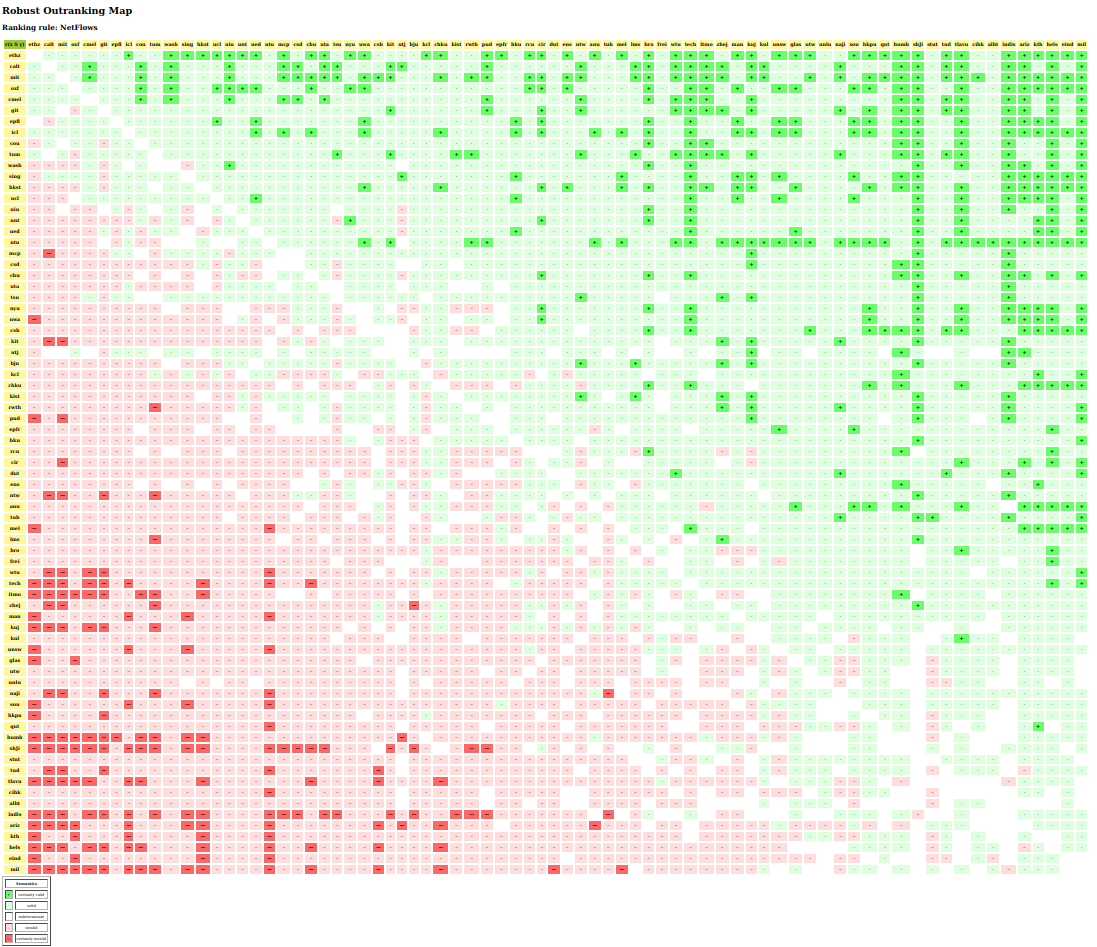
\includegraphics[width=\hsize]{Figures/13-2-the_cs_RelationMap.png}
\caption{Relation map of the robust outranking relation}
\label{fig:13.2}       % Give a unique label
\end{figure}

In Figure~\vref{fig:13.2}, \emph{dark green}, resp. \emph{light green} marked positions show certainly, resp. positively valid outranking situations, whereas \emph{dark red}, resp. \emph{light red} marked positions show certainly, respectively positively valid outranked situations. In the left upper corner one may verify that the five top-ranked Depts ([\texttt{ethz}, \texttt{calt}, \texttt{oxf}, \texttt{mit}, \texttt{cmel}]) are in fact mutually outranking each other and thus are all indifferent one to another. They give even robust \Condorcet winners by robustly outranking all other Depts.

Notice by the way that no certainly valid robust outranking (dark green) and no certainly valid robust outranked situations (dark red) appear in Figure~\vref{fig:13.3} below, resp. above the principal diagonal; none of these robust preferential situations are hence violated by the robust \NetFlows ranking. The non reflexive \emph{white} positions in the relation map, like the one between the Georgia Institute of Technology and the MIT, mark outranking or outranked situations that are not robust with respect to the given significance weight preorder. They become, hence, doubtful and are set to the indeterminate characteristic value $0.0$.

By measuring the ordinal correlation with the underlying pairwise global and marginal robust outranking situations, the quality of the robust \NetFlows ranking result can be formally evaluated with the \texttt{computeRankingCorrelation()} method\index{computeRankingCorrelation@\texttt{computeRankingCorrelation()}} and the \texttt{showCorrelation()} method\index{showCorrelation@\texttt{showCorrelation()}} (see Chap.~\ref{sec:16}).
\begin{lstlisting}[caption={Measuring the quality of the \NetFlows ranking result},label=list:13.13]
>>> corrnf = rdg.computeRankingCorrelation(nfRanking)
>>> rdg.showCorrelation(corrnf)   
  Correlation indexes:
    Crisp ordinal correlation  : +0.901
    Epistemic determination    :  0.563
    Bipolar-valued equivalence : +0.507
\end{lstlisting}

Listing~\vref{list:13.13} Line 4 indicates that the \NetFlows ranking result is indeed highly  correlated ($+0.901$, in \Kendall 's tau index sense) with the pairwise global robust outranking relation. Their bipolar-valued \emph{relational equivalence} index ($+0.51$, Line 6) indicates a more than $75\%$ criteria significance support.

With the \texttt{showRankingConsensusQuality()} method,  we can also check how the \NetFlows ranking rule is actually balancing the five ranking objectives.\index{showRankingConsensusQuality@\texttt{showRankingConsensusQua\-lity()}}
\begin{lstlisting}[caption={Measuring the consensus quality of the \NetFlows ranking result},label=list:13.14]
>>> rdg.showRankingConsensusQuality(nfRanking)
  Criterion (weight): correlation
  -------------------------------
    gtch (0.300): +0.660
    gres (0.300): +0.638
    gcit (0.275): +0.370
    gint (0.075): +0.155
    gind (0.050): +0.101
   Summary:
    Weighted mean marginal correlation (a): +0.508
    Standard deviation (b)                : +0.187
    Ranking fairness (a)-(b)              : +0.321
\end{lstlisting}

The ordinal correlation indexes with the marginal performance criterion rankings are nearly respecting the given significance weights preorder: \texttt{gtch} $\approx$ \texttt{gres} $>$ \texttt{gcit} $>$ \texttt{gint} $>$ \texttt{gind} (see Lines 4-8 above). The mean marginal ordinal correlation index is quite high ($+0.51$). Coupled with a low standard deviation ($0.187$), we obtain a quite fairly balanced ranking result (Lines 10-12). 

We can furthermore inspect with the \texttt{showCriteriaCorrelationTable()} method \index{showCriteriaCorrelationTable@\texttt{showCriteriaCorrelationTable()}} the mutual correlation indexes observed between the individual criterion based marginal robust outranking relations. 
\begin{lstlisting}[caption={Showing the ordinal correlation between the marginal criterion relations},label=list:13.15]
>>> rdg.showCriteriaCorrelationTable()
    Criteria ordinal correlation index
	 |  gcit    gind    gint    gres    gtch   
    -----|------------------------------------------
    gcit | +1.00   -0.11   +0.24   +0.13   +0.17   
    gind |         +1.00   -0.18   +0.15   +0.15   
    gint |                 +1.00   +0.04   -0.00   
    gres |                         +1.00   +0.67   
    gtch |                                 +1.00   
\end{lstlisting}

Slightly contradictory ($-0.11$) appear the \emph{Citations} and \emph{Industrial income} criteria (Line 5 Column 3 in List.~\vref{list:13.15}). Due perhaps to potential confidentiality clauses, it seams perhaps not always possible to publish industrially relevant research results in highly ranked journals. However, criteria \emph{Citations} and \emph{International outlook} show a slightly positive correlation ($+0.24$, Column 4), whereas the \emph{International outlook} criterion shows no apparent correlation with both the major \emph{Teaching} and \emph{Research} criteria. The latter are however highly correlated ($+0.67$. Line 9 Column 6).

A Principal Component Analysis may well illustrate with the \texttt{export3Dplot\-OfCriteriaCorrelation()} method the previous findings \citep{CPSTAT-L2}. \index{export3DplotOfCriteriaCorrelation@\texttt{export3DplotOfCriteria\-Correlation()}}
\begin{lstlisting}
>>> rdg.export3DplotOfCriteriaCorrelation(graphType='pdf')
\end{lstlisting}
\begin{figure}[ht]
%\sidecaption
\includegraphics[width=\hsize]{Figures/13-3-3DCorrelation.pdf}
\caption{3D PCA plot of the pairwise criteria correlation table}
\label{fig:13.3}       % Give a unique label
\end{figure}

In Figure~\vref{fig:13.3}, one may notice first that more than $80\%$ of the total variance of the previous correlation table is explained by the apparent opposition between the marginal outrankings of criteria: \emph{Teaching}, \emph{Research} and \emph{Industry income} on the left side, and the marginal outrankings of criteria: \emph{Citations} and \emph{International outlook} on the right side. Notice also in the left lower corner the nearly identical positions of the marginal outrankings of the major \emph{Teaching} and \emph{Research} criteria. In the factors 2 and 3 plot, about $30\%$ of the total variance is captured by the opposition between the marginal outrankings of the \emph{Teaching} and \emph{Research} criteria and the marginal outrankings of the \emph{Industrial income} criterion. Finally, in the factors 1 and 3 plot, nearly $15\%$ of the total variance is explained by the opposition between the marginal outrankings of the \emph{International outlook} criterion and the marginal outrankings of the \emph{Citations} criterion.

It is, finally, interesting to similarly assess the ordinal correlation between the THE average scores-based ranking and the robust outranking digraph.
\begin{lstlisting}[caption={Computing the ordinal quality of the THE ranking},label=list:13.16]
>>> # theScores = [(xScore_1,x_1), (xScore_2,x_2),... ]
>>> # is sorted in decreasing order of xscores
>>> theRanking = [item[1] for item in theScores]
>>> corrthe = rdg.computeRankingCorrelation(theRanking)
>>> rdg.showCorrelation(corrthe)
    Correlation indexes:
     Crisp ordinal correlation  : +0.907
     Epistemic determination    :  0.563
     Bipolar-valued equivalence : +0.511
>>> rdg.showRankingConsensusQuality(theRanking)
    Criterion (weight): correlation
    -------------------------------
     gtch (0.300): +0.683
     gres (0.300): +0.670
     gcit (0.275): +0.319
     gint (0.075): +0.161
     gind (0.050): +0.106
    Summary:
     Weighted mean marginal correlation (a): +0.511
     Standard deviation (b)                : +0.210
     Ranking fairness (a)-(b)              : +0.302
\end{lstlisting}

The THE ranking result is similarly correlated ($+0.907$, Line 7 in List.~\ref{list:13.16}) with the pairwise global robust outranking situations. By its overall weighted scoring rule, the THE ranking naturally induces marginal criterion correlations that are compatible with the given significance weight preorder (Lines 13-17). Notice that the mean marginal correlation is of a similar value ($+0.51$, Line 19) as the robust \NetFlows ranking. Yet, its standard deviation is slightly higher, which leads to a less fairer balancing of the three major ranking criteria.

To conclude, let us emphasise, that, without any commensurability hypothesis and by taking, furthermore, into account, first, the always present more or less imprecision of any performance evaluation and, secondly, solely ordinal criteria significance weights, we may obtain here with our robust outranking approach a very similar ranking result with a slightly better preference modelling quality. A convincing heatmap view of the 25 first-ranked Institutions may eventually be generated in the default system browser with following command.
\begin{lstlisting}
>>> rdg.showHTMLPerformanceHeatmap(
...            WithActionNames=True,\
...            outrankingModel='this',\
...            rankingRule='NetFlows',\
...            ndigits=1,\
...            Correlations=True,\
...            fromIndex=0,toIndex=25)
\end{lstlisting}
\begin{figure}[ht]
%\sidecaption
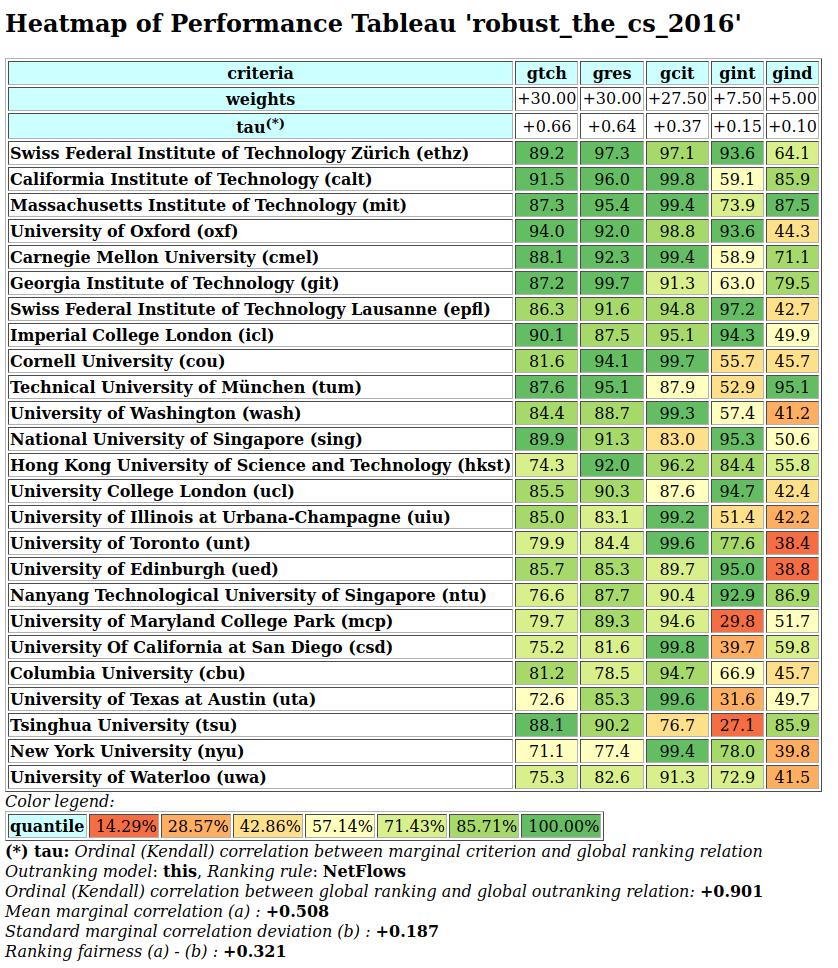
\includegraphics[width=\hsize]{Figures/13-4-theHeatmap.png}
\caption{Extract of a heatmap browser view on the \NetFlows ranking result}
\label{fig:13.4}       % Give a unique label
\end{figure}

As an exercise, the reader is invited to try out other robust outranking based ranking heuristics. Notice also that we have not challenged in this case study the THE provided criteria significance preorder. It would be very interesting to consider the five ranking objectives as equally important and, consequently, consider the ranking criteria to be equisignificant. Curious to see the ranking results under such settings.
 
%%%%%%% The chapter bibliography
%\normallatexbib
%\clearpage
\phantomsection
\addcontentsline{toc}{section}{Chapter Bibliography}
\input{02-mainMatters/13-chapterBestCSDpts.bbl}
%\bibliographystyle{spbasic}
%\bibliography{03-backMatters/reference}

%\bibliographystyle{spbasic}
%\bibliography{03-backMatters/reference}

%\bibliographystyle{spbasic}
%\bibliography{03-backMatters/reference}
